\documentclass[letterpaper,twocolumn,10pt]{article}
\usepackage{usenix2019_v3} % For I have become death; destroyer of style files
%\usepackage{HACKED_FOR_NO_AUTHORS_usenix2019_v3} % For I have become death; destroyer of style files

%\documentclass[10pt,sigconf,letterpaper,prologue,dvipsnames]{acmart}
%\documentclass{article}
\usepackage{adjustbox}
\usepackage{amssymb}
\usepackage{amsmath}
\usepackage{multicol}
\usepackage{supertabular}
\usepackage{tikz,graphicx,balance,multirow,xspace,subcaption,longtable}
\usepackage{makecell,amsmath,cleveref,rotating}
%\usepackage[font={small}, textfont=md]{caption}
\usepackage[T1]{fontenc}
\usepackage{enumitem}
\usepackage[draft,inline,nomargin,index]{fixme}
\usepackage{booktabs}
\usepackage{lastpage}
\usepackage{titling}
\usepackage{xcolor,colortbl}

\usepackage{enumitem}
\setitemize{noitemsep,topsep=0pt,parsep=0pt,partopsep=0pt}


% And now we bring you to the Paul Does Crimes portion of the evening
\usepackage[font={small}, textfont=md, skip=.2pt]{caption} % the commented version of this above is the original 
% \setlength{\textfloatsep}{18pt plus 2pt minus 1pt}
 \setlength{\floatsep}{4pt plus 1pt minus 1pt}
% \usepackage[compact]{titlesec}
\newcommand{\tabularscale}{0.80}

\PassOptionsToPackage{hyphens}{url}
\usepackage{hyperref}
\urlstyle{tt}
\newcolumntype{P}[1]{>{\arraybackslash}p{#1}}
\newcolumntype{X}[1]{>{\centering\arraybackslash}p{#1}}

\expandafter\def\expandafter\UrlBreaks\expandafter{\UrlBreaks%  save the current one
  \do\a\do\b\do\c\do\d\do\e\do\f\do\g\do\h\do\i\do\j%
  \do\k\do\l\do\m\do\n\do\o\do\p\do\q\do\r\do\s\do\t%
  \do\u\do\v\do\w\do\x\do\y\do\z\do\A\do\B\do\C\do\D%
  \do\E\do\F\do\G\do\H\do\I\do\J\do\K\do\L\do\M\do\N%
  \do\O\do\P\do\Q\do\R\do\S\do\T\do\U\do\V\do\W\do\X%
  \do\Y\do\Z}


\crefformat{section}{\S#2#1#3}
\crefformat{subsection}{\S#2#1#3}
\crefformat{subsubsection}{\S#2#1#3}

\fxsetup{theme=colorsig,mode=multiuser,inlineface=\itshape,envface=\itshape}
\FXRegisterAuthor{ht}{aht}{Hammas}
\FXRegisterAuthor{rn}{arn}{Rishab}
\FXRegisterAuthor{rs}{ars}{Rachee}
\FXRegisterAuthor{pp}{app}{Paul}

\hypersetup{%
  pdftitle={},
  pdfauthor={},
  pdfkeywords={},
  bookmarksnumbered,
  pdfstartview={FitH},
  colorlinks,
  citecolor=black,
  filecolor=black,
  linkcolor=black,
  urlcolor=blue,
  breaklinks=true,
  hypertexnames=false
}

\newcommand\setrow[1]{\gdef\rowmac{#1}#1\ignorespaces}
\newcommand\clearrow{\global\let\rowmac\relax}

\clubpenalty=10000
\widowpenalty=10000


\newcommand{\para}[1]{{\vspace{.05in} \bf \noindent #1 }}
\newcommand{\parait}[1]{{\vspace{.05in} \em \noindent #1 }}
\newcommand{\FIXME}[1] {\textcolor{blue}{[\textbf{FIXME: } \emph{#1}]}}
\newcommand{\subnet}[1]{\texttt{/#1}}

\newcommand{\Cg}{$\mathcal{C}$\xspace}
\newcommand{\Tg}[1]{$\mathcal{T}_{{\text{#1}}}$\xspace}
\newcommand{\rate}{$\mathcal{\mu}$\xspace}
\newcommand{\ddiff}[1]{$\Delta_{#1}^{\text{diff}}$\xspace}
\newcommand{\dcontrol}[1]{$\Delta_{#1}^{\text{\Cg}}$\xspace}
\newcommand{\meanscansperday}[2]{$\text{\rate}^{({#1})}_{\text{{#2}}}$\xspace}

\newcommand{\red}[1]{\textcolor{red}{\bf #1}}
\newcommand{\blue}[1]{\textcolor{blue}{\bf #1}}

\newenvironment{packed_itemize}{
\begin{itemize}
  \setlength{\itemsep}{2pt}
  \setlength{\parskip}{0pt}
  \setlength{\parsep}{0pt}
  \setlength{\topsep}{2pt}
}{\end{itemize}}

\newenvironment{packed_enumerate}{
\begin{enumerate}
  \setlength{\itemsep}{2pt}
  \setlength{\parskip}{0pt}
  \setlength{\parsep}{0pt}
  \setlength{\topsep}{2pt}
}{\end{enumerate}}

\renewcommand{\footnotesize}{\scriptsize}
\newcommand{\Sidak}{\v{S}id\'{a}k\ }
\newcommand{\etc}{etc.}
\newcommand{\eg}{e.g.,\ }
\newcommand{\etal}{et al.\xspace}
\newcommand{\ie}{i.e.,\ }
\newcommand{\re}{r.e.\ }
\newcommand{\aka}{a.k.a.\ }
\newcommand{\cf}{\emph{cf.,\ }}
\newcommand{\nx}{{NXDOMAIN}\xspace}

\newcommand{\plb}{$P_{l}$\xspace}
\newcommand{\prb}{$P_{r}$\xspace}
\newcommand{\slb}{$S_{l}$\xspace}
\newcommand{\srb}{$S_{r}$\xspace}

\newcommand{\lb}{\textit{lower-byte}\ }
\newcommand{\rnd}{\textit{random}\ }
\newcommand{\tr}{\textit{Treatment}\ }
\newcommand{\nb}{\textit{Neighbor}\ }
\newcommand{\ot}{\textit{Control}\ }
\newcommand{\nyb}{\textit{nybble}\ }
\newcommand{\nybs}{\textit{nybbles}\ }

\providecommand{\superem}[1]{\underline{\emph{#1}}}


% \copyrightyear{2019} 
% \acmYear{2018} 
% \setcopyright{acmlicensed}
% \acmConference[IMC '19]{acm}{imc}
% \acmBooktitle{title}
% \acmPrice{price}
% \acmDOI{doi}
% \acmISBN{isbc}

% \settopmatter{printacmref=false}
% \setcopyright{none}

% \newcommand{\FigIdentifySender}{
% \begin{figure}[t]
%     \centering
%     \includegraphics[width=0.9\linewidth]{figures/linegraph.png}
%     \caption{\textbf{Messages needed to identify sender}\,---\,% 
%         We measured the number of epochs that were necessary for an attacker to
%         uniquely determine who was messaging a pre-selected victim, Bob, under
%         sealed sender assuming every message was ``immediately'' replied to with
%         a \textit{delivery receipt}. We found that the graph structure had no
%         influence on the effectiveness of the attack. We ran the attack 100
%         times for each user base size and found that with a user base of
%         1,000,000 on average Bob needed to receive 6.5 message from the same
%         user in order to deanonymize the conversation between the sender (Alice)
%         and Bob.
%         }
%     \label{fig:NumMessages}
% \end{figure}
% }

\newcommand{\SmallCountriesCorporate}{
    \begin{table}[t]
        \centering
        \small
        \scalebox{0.6}{
            \begin{tabular}{ccccccc}
                \toprule\textbf{Country} & \textbf{Resolver Pairs} & \textbf{IPv4 A} & \textbf{IPv4 AAAA} & \textbf{IPv6 A} & \textbf{IPv6 AAAA} & \textbf{Avg.}\\\midrule
                United States (US) & 757 & 1.62 & 1.16 & 0.54 & 0.96 & 1.07\\
                Germany (DE) & 717 & 0.98 & 0.91 & 0.75 & 0.80 & 0.86\\
                France (FR) & 470 & 0.60 & 0.45 & 0.40 & 0.46 & 0.48\\
                Great Britan (GB) & 186 & 1.07 & 0.94 & 0.78 & 0.97 & 0.94\\
                South Korea (KR) & 177 & 2.49 & 1.37 & 1.38 & 1.57 & 1.70\\
                Canada (CA) & 165 & 0.84 & 0.39 & 0.26 & 0.33 & 0.45\\
                Russia (RU) & 117 & 4.67 & 4.36 & 4.01 & 4.00 & 4.26\\
                India (IN) & 101 & 1.19 & 1.76 & 0.81 & 0.99 & 1.19\\
                Japan (JP) & 79 & 1.71 & 1.82 & 0.90 & 1.57 & 1.50\\
                South Africa (ZA) & 74 & 2.09 & 1.62 & 1.10 & 1.31 & 1.53\\
                Netherlands (NL) & 71 & 1.08 & 0.94 & 0.84 & 0.85 & 0.92\\
                Chile (CL) & 53 & 2.10 & 0.73 & 1.12 & 0.77 & 1.18\\
                Lithuania (LT) & 51 & 0.95 & 0.80 & 0.51 & 0.78 & 0.76\\
                Iran (IR) & 48 & 25.50 & 24.66 & 22.34 & 21.69 & 23.55\\
                Thailand (TH) & 43 & 9.28 & 1.18 & 0.99 & 0.95 & 3.10\\
                Singapore (SG) & 41 & 1.56 & 0.85 & 0.65 & 0.78 & 0.96\\
                Viet Nam (VN) & 40 & 2.16 & 1.01 & 0.85 & 0.86 & 1.22\\
                Hong Kong (HK) & 37 & 6.20 & 5.44 & 4.55 & 5.38 & 5.39\\
                Austrailia (AU) & 35 & 2.53 & 1.16 & 1.77 & 1.14 & 1.65\\
                Brazil (BR) & 34 & 1.50 & 1.10 & 1.01 & 1.17 & 1.19\\
                Finland (FI) & 31 & 0.74 & 0.64 & 0.47 & 0.56 & 0.60\\
                Malaysia (MY) & 30 & 6.07 & 2.25 & 0.97 & 1.10 & 2.60\\
                Spain (ES) & 28 & 1.26 & 0.97 & 2.24 & 2.97 & 1.86\\
                Turkey (TR) & 25 & 1.72 & 1.29 & 1.20 & 2.17 & 1.60\\
                \bottomrule
            \end{tabular}} 
            \caption{
                We highlight the countries with at least 25 resolver pairs in
                corporate ASes to showcase their censorship rates across
                interface and resource type. We see this is where the
                predominant censorship in the United States is present. 
            }
            \label{tab:small-countries-corporate}
    \end{table}
}


\newcommand{\IranRecursionTable}{
\begin{table}[h!]
    \begin{center}
        \begin{tabular}{l|c|c|c} % <-- Alignments: 1st column left, 2nd middle and 3rd right, with vertical lines in between
                  & \textbf{V4} & \textbf{V6} & \textbf{6to4}         \\
            \hline
            RD    & 10.10.34.35 & d0::11      & 10.10.34.35           \\
            No RD & 10.10.34.35 & d0::11      & \textbf{no injection} \\
        \end{tabular}
    \end{center}
    \caption{The Iranian censor provides distinctive injections to queries sent
        over both v4 and v6, but fails to inject responses for queries to
        resolvers using 6to4 addresses when the query excludes the recursion
        desired flag.}
    \label{tab:iran-recursion-table}
\end{table}
}

\newcommand{\CountriesCorporate}{
    \begin{table*}[ht]
        \centering
        {\tiny\renewcommand{\arraystretch}{.8}
        \resizebox{!}{.35\paperheight}{%
            \begin{tabular}{cccccccc}
                \toprule\textbf{Country} & \textbf{Network Type} & \textbf{Resolver Pairs} & \textbf{IPv4 A} & \textbf{IPv4 AAAA} & \textbf{IPv6 A} & \textbf{IPv6 AAAA} & \textbf{Avg.}\\\midrule
                CN & Total & 194 & 29.27 & 32.32 & 28.41 & 32.08 & 30.52\\                                                                                                                                                         
                CN & Corporate & 15 & 26.96 & 28.05 & 23.44 & 26.16 & 26.15\\                                                                                                                                                      
                CN & Non Corporate & 179 & 29.46 & 32.68 & 28.82 & 32.58 & 30.89\\                                                                                                                                                 
                \midrule                                                                                                                                                                                                           
                IR & Total & 277 & 25.12 & 24.49 & 21.95 & 21.45 & 23.25\\                                                                                                                                                         
                IR & Corporate & 48 & 25.50 & 24.66 & 22.34 & 21.69 & 23.55\\                                                                                                                                                      
                IR & Non Corporate & 229 & 25.04 & 24.46 & 21.87 & 21.40 & 23.19\\                                                                                                                                                 
                \midrule                                                                                                                                                                                                           
                HK & Total & 67 & 7.00 & 5.57 & 4.91 & 5.24 & 5.68\\                                                                                                                                                               
                HK & Corporate & 37 & 6.20 & 5.44 & 4.55 & 5.38 & 5.39\\                                                                                                                                                           
                HK & Non Corporate & 30 & 8.00 & 5.74 & 5.35 & 5.08 & 6.04\\                                                                                                                                                       
                \midrule                                                                                                                                                                                                           
                RU & Total & 312 & 5.51 & 4.78 & 4.49 & 4.50 & 4.82\\                                                                                                                                                              
                RU & Corporate & 117 & 4.67 & 4.36 & 4.01 & 4.00 & 4.26\\                                                                                                                                                          
                RU & Non Corporate & 195 & 6.02 & 5.03 & 4.78 & 4.80 & 5.16\\                                                                                                                                                      
                \midrule                                                                                                                                                                                                           
                UA & Total & 35 & 6.49 & 3.05 & 2.64 & 2.87 & 3.76\\                                                                                                                                                               
                UA & Corporate & 11 & 4.39 & 1.25 & 1.02 & 1.87 & 2.13\\                                                                                                                                                           
                UA & Non Corporate & 24 & 7.46 & 3.87 & 3.38 & 3.33 & 4.51\\                                                                                                                                                       
                \midrule                                                                                                                                                                                                           
                ID & Total & 56 & 6.46 & 2.99 & 2.41 & 2.26 & 3.53\\                                                                                                                                                               
                ID & Corporate & 16 & 6.92 & 3.38 & 3.02 & 2.83 & 4.04\\                                                                                                                                                           
                ID & Non Corporate & 40 & 6.27 & 2.84 & 2.17 & 2.04 & 3.33\\                                                                                                                                                       
                \midrule                                                                                                                                                                                                           
                AR & Total & 47 & 5.20 & 3.51 & 2.22 & 1.28 & 3.05\\                                                                                                                                                               
                AR & Corporate & 13 & 4.47 & 1.64 & 1.31 & 1.20 & 2.15\\                                                                                                                                                           
                AR & Non Corporate & 34 & 5.47 & 4.22 & 2.56 & 1.31 & 3.39\\                                                                                                                                                       
                \midrule                                                                                                                                                                                                           
                TH & Total & 186 & 8.25 & 1.18 & 1.13 & 0.93 & 2.87\\                                                                                                                                                              
                TH & Corporate & 43 & 9.28 & 1.18 & 0.99 & 0.95 & 3.10\\                                                                                                                                                           
                TH & Non Corporate & 143 & 7.94 & 1.18 & 1.17 & 0.93 & 2.80\\                                                                                                                                                      
                \midrule                                                                                                                                                                                                           
                MY & Total & 50 & 4.92 & 2.03 & 1.27 & 1.35 & 2.39\\                                                                                                                                                               
                MY & Corporate & 30 & 6.07 & 2.25 & 0.97 & 1.10 & 2.60\\                                                                                                                                                           
                MY & Non Corporate & 20 & 3.18 & 1.68 & 1.72 & 1.72 & 2.07\\                                                                                                                                                       
                \midrule                                                                                                                                                                                                           
                MX & Total & 150 & 3.78 & 2.05 & 1.75 & 1.94 & 2.38\\                                                                                                                                                              
                MX & Corporate & 10 & 2.04 & 2.27 & 2.41 & 2.54 & 2.31\\                                                                                                                                                           
                MX & Non Corporate & 140 & 3.90 & 2.03 & 1.70 & 1.89 & 2.38\\                                                                                                                                                      
                \midrule                                                                                                                                                                                                           
                BD & Total & 29 & 6.42 & 1.28 & 0.89 & 0.81 & 2.35\\                                                                                                                                                               
                BD & Corporate & 0 & 0.00 & 0.00 & 0.00 & 0.00 & 0.00\\
                BD & Non Corporate & 29 & 6.42 & 1.28 & 0.89 & 0.81 & 2.35\\
                \midrule
                CO & Total & 27 & 3.39 & 3.28 & 1.45 & 1.14 & 2.31\\ 
                CO & Corporate & 2 & 0.21 & 0.28 & 0.21 & 0.84 & 0.39\\
                CO & Non Corporate & 25 & 3.64 & 3.52 & 1.55 & 1.16 & 2.47\\
                \midrule
                IT & Total & 38 & 2.36 & 2.10 & 2.25 & 2.52 & 2.31\\ 
                IT & Corporate & 23 & 2.55 & 2.20 & 1.57 & 1.78 & 2.02\\
                IT & Non Corporate & 15 & 2.05 & 1.96 & 3.29 & 3.67 & 2.74\\
                \midrule
                BR & Total & 160 & 2.67 & 1.67 & 1.99 & 2.08 & 2.10\\
                BR & Corporate & 34 & 1.50 & 1.10 & 1.01 & 1.17 & 1.19\\
                BR & Non Corporate & 126 & 2.99 & 1.82 & 2.25 & 2.33 & 2.35\\
                \midrule
                BG & Total & 30 & 3.24 & 2.91 & 1.15 & 1.06 & 2.09\\
                BG & Corporate & 11 & 3.78 & 1.92 & 1.49 & 1.29 & 2.12\\
                BG & Non Corporate & 19 & 2.92 & 3.49 & 0.95 & 0.94 & 2.07\\
                \midrule
                PL & Total & 48 & 2.00 & 1.13 & 2.90 & 0.96 & 1.75\\
                PL & Corporate & 16 & 2.60 & 1.58 & 4.82 & 1.42 & 2.61\\
                PL & Non Corporate & 32 & 1.71 & 0.91 & 1.93 & 0.74 & 1.32\\
                \midrule
                ZA & Total & 93 & 2.41 & 1.60 & 1.18 & 1.33 & 1.63\\
                ZA & Corporate & 74 & 2.09 & 1.62 & 1.10 & 1.31 & 1.53\\
                ZA & Non Corporate & 19 & 3.64 & 1.53 & 1.48 & 1.42 & 2.02\\
                \midrule
                KR & Total & 632 & 2.33 & 1.06 & 1.24 & 1.22 & 1.46\\
                KR & Corporate & 177 & 2.49 & 1.37 & 1.38 & 1.57 & 1.70\\
                KR & Non Corporate & 455 & 2.26 & 0.94 & 1.19 & 1.09 & 1.37\\
                \midrule
                CL & Total & 65 & 2.67 & 0.70 & 1.10 & 0.79 & 1.32\\
                CL & Corporate & 53 & 2.10 & 0.73 & 1.12 & 0.77 & 1.18\\
                CL & Non Corporate & 12 & 5.17 & 0.58 & 1.00 & 0.91 & 1.92\\
                \midrule
                RO & Total & 44 & 2.30 & 1.03 & 0.83 & 0.93 & 1.27\\
                RO & Corporate & 6 & 2.17 & 0.58 & 0.47 & 0.63 & 0.96\\
                RO & Non Corporate & 38 & 2.32 & 1.10 & 0.89 & 0.97 & 1.32\\
                \midrule
                ES & Total & 49 & 0.91 & 0.75 & 1.40 & 1.94 & 1.25\\
                ES & Corporate & 28 & 1.26 & 0.97 & 2.24 & 2.97 & 1.86\\
                ES & Non Corporate & 21 & 0.46 & 0.47 & 0.29 & 0.58 & 0.45\\
                \midrule
                IN & Total & 226 & 1.27 & 1.52 & 1.04 & 1.16 & 1.25\\
                IN & Corporate & 101 & 1.19 & 1.76 & 0.81 & 0.99 & 1.19\\
                IN & Non Corporate & 125 & 1.34 & 1.32 & 1.23 & 1.30 & 1.30\\
                \midrule
                BE & Total & 31 & 1.56 & 1.26 & 0.95 & 0.95 & 1.18\\
                BE & Corporate & 4 & 1.33 & 1.30 & 1.16 & 1.26 & 1.26\\
                BE & Non Corporate & 27 & 1.59 & 1.25 & 0.92 & 0.91 & 1.17\\
                \midrule
                TR & Total & 114 & 1.29 & 0.96 & 1.27 & 1.02 & 1.14\\
                TR & Corporate & 25 & 1.72 & 1.29 & 1.20 & 2.17 & 1.60\\
                TR & Non Corporate & 89 & 1.17 & 0.86 & 1.29 & 0.70 & 1.01\\
                \midrule
                VN & Total & 252 & 1.53 & 0.89 & 1.42 & 0.67 & 1.13\\
                VN & Corporate & 40 & 2.16 & 1.01 & 0.85 & 0.86 & 1.22\\
                VN & Non Corporate & 212 & 1.42 & 0.86 & 1.52 & 0.64 & 1.11\\
                \bottomrule
            \end{tabular}}}
    \end{table*}
}

\newcommand{\IRTopDomainTable}{
    \begin{table}[t]
        \centering
        \begin{adjustbox}{width=\textwidth}
            \begin{tabular}{|c||ccc|}
                \hline\textbf{Domain} & \textbf{Requested Record Type} & \textbf{Number of Censoring v4 Resolvers} & \textbf{Number of Censoring v6 Resolvers}\\\hline
                secure.flickr.com & A & 276 & 209\\
                www.netflix.com & A & 275 & 206\\
                yumpu.com & A & 276 & 204\\
                www.urduvoa.com & A & 276 & 204\\
                www.snapchat.com & A & 274 & 206\\
                www.ning.com & A & 276 & 204\\
                www.lightsailvpn.com & A & 276 & 204\\
                signal.org & A & 275 & 205\\
                www.vonage.com & A & 276 & 203\\
                www.voanews.com & A & 276 & 203\\
                \hline
            \end{tabular}
        \end{adjustbox}
        \caption{\textbf{Iran table of most censored domains}\,---\,%
            We measured which domains were blocked in Iran, and whether they were
            blocked differently between resolvers at a v4 IP address, compared to
            those at a v6 IP address. As we can see here the most popularly blocked
            domains are blocked by resolvers on different IP address families but
            there is a difference. These domains were blocked by the most resolvers.
        }
        \label{tab:ir-top}
    \end{table}
}

\newcommand{\IRDifferenceDomainTable}{
    \begin{table}[ht]
        \centering
        \begin{adjustbox}{width=\textwidth}
            \begin{tabular}{|c||ccc|}
                \hline\textbf{Domain} & \textbf{Requested Record Type} & \textbf{Number of Censoring v4 Resolvers} & \textbf{Number of Censoring v6 Resolvers}\\\hline
                www.nbc.com & AAAA & 261 & 25\\
                download.cnet.com & AAAA & 259 & 23\\
                www.indiatimes.com & AAAA & 262 & 28\\
                spankbang.com & AAAA & 261 & 27\\
                psiphon.ca & AAAA & 261 & 27\\
                free.fr & AAAA & 261 & 27\\
                www.voanews.com & AAAA & 261 & 28\\
                www.netflix.com & AAAA & 262 & 29\\
                www.jesussaves.cc & AAAA & 261 & 28\\
                tmz.com & AAAA & 264 & 31\\
                \hline
            \end{tabular}
        \end{adjustbox}
        \caption{\textbf{Iran table of most difference in Address Family Censorship}\,---\,%
            We measured which domains were blocked in Iran, and whether they were
            blocked differently between resolvers at a v4 IP address, compared to
            those at a v6 IP address. As we can see here the most popularly blocked
            domains are blocked by resolvers on different IP address families but
            there is a difference. These domains had the largest difference in
            censoring behavior between resolver address family. 
        }
        \label{tab:ir-diff}
    \end{table}
}

\newcommand{\RUTopDomainTable}{
    \begin{table}[ht]
        \centering
        \begin{adjustbox}{width=\textwidth}
            \begin{tabular}{|c||ccc|}
                \hline\textbf{Domain} & \textbf{Requested Record Type} & \textbf{Number of Censoring v4 Resolvers} & \textbf{Number of Censoring v6 Resolvers}\\\hline
                eenadu.net & AAAA & 148 & 89\\
                www.spotify.com & AAAA & 93 & 98\\
                www.ned.org & A & 60 & 29\\
                www.europacasino.com & A & 47 & 37\\
                www.casinotropez.com & A & 45 & 37\\
                global.blackberry.com & A & 44 & 34\\
                www.sex.com & A & 40 & 37\\
                www.khilafah.com & A & 40 & 37\\
                ultrasurf.us & A & 41 & 36\\
                thepiratebay.org & A & 39 & 38\\
                \hline
            \end{tabular}
        \end{adjustbox}
        \caption{\textbf{Russia's top censored domains}\,---\,%
        }
        \label{tab:ru-top}
    \end{table}
}

\newcommand{\RUDifferenceDomainTable}{
    \begin{table}[ht]
        \centering
        \begin{adjustbox}{width=\textwidth}
            \begin{tabular}{|c||ccc|}
                \hline\textbf{Domain} & \textbf{Requested Record Type} & \textbf{Number of Censoring v4 Resolvers} & \textbf{Number of Censoring v6 Resolvers}\\\hline
                eenadu.net & AAAA & 148 & 89\\
                doh.dns.sb & A & 36 & 4\\
                www.ned.org & A & 60 & 29\\
                www.volcanomail.com & A & 30 & 0\\
                www.msf.org & A & 24 & 0\\
                mail.yahoo.com & A & 24 & 1\\
                www.cnn.com & AAAA & 0 & 21\\
                www.netflix.com & A & 27 & 10\\
                www.theglobalfund.org & A & 20 & 5\\
                www.ecdc.europa.eu & A & 15 & 0\\
                \hline
            \end{tabular}
        \end{adjustbox}
        \caption{\textbf{Russia's biggest difference domains}\,---\,%
        }
        \label{tab:ru-diff}
    \end{table}
}

\newcommand{\HKTopDomainTable}{
    \begin{table}[ht]
        \centering
        \begin{adjustbox}{width=\textwidth}
            \begin{tabular}{|c||ccc|}
                \hline\textbf{Domain} & \textbf{Requested Record Type} & \textbf{Number of Censoring v4 Resolvers} & \textbf{Number of Censoring v6 Resolvers}\\\hline
                eenadu.net & AAAA & 26 & 15\\
                www.ned.org & A & 14 & 3\\
                www.gov.uk & A & 12 & 2\\
                www.netflix.com & A & 11 & 2\\
                www.bittorrent.com & A & 10 & 2\\
                google.com.co & AAAA & 5 & 6\\
                www.nro.gov & A & 6 & 4\\
                www.terredeshommes.nl & A & 7 & 2\\
                mail.yahoo.com & A & 8 & 1\\
                google.ro & AAAA & 6 & 3\\
                \hline
            \end{tabular}
        \end{adjustbox}
        \caption{\textbf{Hong Kong's most censored domains}\,---\,%
        }
        \label{tab:hk-top}
    \end{table}
}

\newcommand{\HKDifferenceDomainTable}{
    \begin{table}[ht]
        \centering
        \begin{adjustbox}{width=\textwidth}
            \begin{tabular}{|c||ccc|}
                \hline\textbf{Domain} & \textbf{Requested Record Type} & \textbf{Number of Censoring v4 Resolvers} & \textbf{Number of Censoring v6 Resolvers}\\\hline
                www.ned.org & A & 14 & 3\\
                eenadu.net & AAAA & 26 & 15\\
                www.gov.uk & A & 12 & 2\\
                www.netflix.com & A & 11 & 2\\
                www.bittorrent.com & A & 10 & 2\\
                mail.yahoo.com & A & 8 & 1\\
                www.utorrent.com & A & 7 & 1\\
                www.ftchinese.com & A & 6 & 0\\
                www.familyequality.org & A & 7 & 1\\
                it.wikipedia.org & A & 6 & 0\\
                \hline
            \end{tabular}
        \end{adjustbox}
        \caption{\textbf{Hong Kong's biggest difference domains}\,---\,%
        }
        \label{tab:hk-diff}
    \end{table}
}

\newcommand{\CNTopDomainTable}{
    \begin{table}[ht]
        \centering
        \begin{adjustbox}{width=\textwidth}
            \begin{tabular}{|c||ccc|}
                \hline\textbf{Domain} & \textbf{Requested Record Type} & \textbf{Number of Censoring v4 Resolvers} & \textbf{Number of Censoring v6 Resolvers}\\\hline
                google.com.co & AAAA & 188 & 189\\
                google.co.in & AAAA & 189 & 188\\
                youtube.com & AAAA & 188 & 188\\
                www.ned.org & A & 189 & 187\\
                www.google.com & AAAA & 188 & 188\\
                www.blogger.com & AAAA & 188 & 188\\
                ultrasurf.us & AAAA & 188 & 188\\
                sites.google.com & AAAA & 188 & 188\\
                plus.google.com & AAAA & 188 & 188\\
                groups.google.com & AAAA & 188 & 188\\
                \hline
            \end{tabular}
        \end{adjustbox}
        \caption{\textbf{China's most censored domains}\,---\,%
        }
        \label{tab:cn-top}
    \end{table}
}

\newcommand{\CNDifferenceDomainTable}{
    \begin{table}[ht]
        \centering
        \begin{adjustbox}{width=\textwidth}
            \begin{tabular}{|c||ccc|}
                \hline\textbf{Domain} & \textbf{Requested Record Type} & \textbf{Number of Censoring v4 Resolvers} & \textbf{Number of Censoring v6 Resolvers}\\\hline
                google.com & A & 168 & 122\\
                google.com & AAAA & 180 & 145\\
                www.glaad.org & A & 30 & 6\\
                eenadu.net & AAAA & 116 & 96\\
                www.lanacion.com.ar & A & 20 & 1\\
                premierbet.co.ao & A & 25 & 7\\
                www.familyequality.org & A & 17 & 2\\
                www.bittorrent.com & A & 18 & 4\\
                qalam.withgoogle.com & A & 2 & 16\\
                global.blackberry.com & A & 16 & 2\\
                \hline
            \end{tabular}
        \end{adjustbox}
        \caption{\textbf{China's biggest difference domains}\,---\,%
        }
        \label{tab:cn-diff}
    \end{table}
}


% colors for the table below
%\definecolor{red0}{rgb}{1,0.9,0.9}
%\definecolor{red1}{rgb}{1,0.8,0.8}
%\definecolor{red2}{rgb}{1,0.7,0.7}
%\definecolor{red3}{rgb}{1,0.6,0.6}
%\definecolor{red4}{rgb}{1,0.5,0.5}
%\definecolor{red5}{rgb}{1,0.4,0.4}
%\definecolor{green0}{rgb}{0.9,1,0.9}
%\definecolor{green1}{rgb}{0.8,1,0.8}
%\definecolor{green2}{rgb}{0.7,1,0.7}
\definecolor{red00}{rgb}{1,0.9,0.9}
\definecolor{red0}{rgb}{1,0.8,0.8}
\definecolor{red1}{rgb}{1,0.7,0.7}
\definecolor{red2}{rgb}{1,0.6,0.6}
\definecolor{red3}{rgb}{1,0.5,0.5}
\definecolor{red4}{rgb}{1,0.4,0.4}
\definecolor{red5}{rgb}{1,0.3,0.3}
%\definecolor{green0}{rgb}{0.9,1,0.9}
\definecolor{green0}{rgb}{0.8,1,0.8}
\definecolor{green1}{rgb}{0.7,1,0.7}
\definecolor{green2}{rgb}{0.6,1,0.6}
\definecolor{green3}{rgb}{0.5,1,0.5}
\definecolor{green4}{rgb}{0.4,1,0.4}
\definecolor{green5}{rgb}{0.3,1,0.3}




\newcommand{\TabBaseRate}{
    \begin{table}[ht]
        \centering
        \small
        \scalebox{\tabularscale} {
        \begin{tabular}{lccccc}
            \toprule
                %\textbf{Country} & \textbf{Resolver pairs} & \textbf{v4/A} & \textbf{v4/AAAA} & \textbf{v6/A} & \textbf{v6/AAAA} \\
                \textbf{} & \textbf{Resolver} & \textbf{IPv4} & \textbf{IPv4} & \textbf{IPv6} & \textbf{IPv6} \\
                \textbf{Country} & \textbf{pairs} & \textbf{A} & \textbf{AAAA} & \textbf{A} & \textbf{AAAA} \\
                \midrule

United States (US)    &   1228  & 1.4\% & 0.9\% & 0.5\% & 0.9\% \\  % avg 0.9 stdev 2.6
Germany (DE)          &   753  & 1.0\% & 0.9\% & 0.8\% & 0.8\% \\  % avg 0.9 stdev 3.3
South Korea (KR)      &   632  & \cellcolor{red0} 2.3\% & 1.1\% & 1.2\% & 1.2\% \\  % avg 1.5 stdev 2.9
France (FR)           &   560  & 0.6\% & 0.5\% & 0.4\% & 0.6\% \\  % avg 0.5 stdev 1.8
Russia (RU)           &   312  & 5.5\% & 4.8\% & 4.5\% & 4.5\% \\  % avg 4.8 stdev 3.6
Iran (IR)             &   277  & \cellcolor{red1} 25.1\% & \cellcolor{red0} 24.5\% & \cellcolor{green0} 22.0\% & \cellcolor{green1} 21.4\% \\  % avg 23.3 stdev 3.4
Vietnam (VN)          &   252  & 1.5\% & 0.9\% & 1.4\% & 0.7\% \\  % avg 1.1 stdev 1.9
Taiwan (TW)           &   248  & 1.2\% & 1.0\% & 0.9\% & 0.9\% \\  % avg 1.0 stdev 4.0
India (IN)            &   226  & 1.3\% & 1.5\% & 1.0\% & 1.2\% \\  % avg 1.2 stdev 1.4
Canada (CA)           &   199  & \cellcolor{red0} 0.7\% & 0.4\% & 0.2\% & 0.3\% \\  % avg 0.4 stdev 1.2
United Kingdom (GB)   &   196  & 1.1\% & 0.9\% & 0.8\% & 1.0\% \\  % avg 1.0 stdev 3.3
China (CN)            &   194  & 29.3\% & \cellcolor{red0} 32.3\% & \cellcolor{green0} 28.4\% & \cellcolor{red0} 32.1\% \\  % avg 30.5 stdev 5.9
Thailand (TH)         &   186  & \cellcolor{red5}  8.2\% & \cellcolor{green0} 1.2\% & \cellcolor{green0} 1.1\% & \cellcolor{green0} 0.9\% \\  % avg 2.9 stdev 4.3
Brazil (BR)           &   160  & 2.7\% & 1.7\% & 2.0\% & 2.1\% \\  % avg 2.1 stdev 4.7
Japan (JP)            &   152  & 1.1\% & 1.2\% & 0.6\% & 1.0\% \\  % avg 1.0 stdev 3.4
Mexico (MX)           &   150  & \cellcolor{red0} 3.8\% & 2.0\% & 1.7\% & 1.9\% \\  % avg 2.4 stdev 5.0
Turkey (TR)           &   114  & 1.3\% & 1.0\% & 1.3\% & 1.0\% \\  % avg 1.1 stdev 3.2
Netherlands (NL)      &    97  & 1.2\% & 0.8\% & 0.7\% & 0.7\% \\  % avg 0.8 stdev 2.3
South Africa (ZA)     &    93  & 2.4\% & 1.6\% & 1.2\% & 1.4\% \\  % avg 1.6 stdev 4.2
Australia (AU)        &    72  & 1.6\% & 0.7\% & 0.9\% & 0.7\% \\  % avg 1.0 stdev 2.9
Hong Kong (HK)        &    67  & \cellcolor{red0} 7.0\% & 5.6\% & 4.9\% & 5.2\% \\  % avg 5.7 stdev 4.9
Chile (CL)            &    65  & \cellcolor{red1} 2.7\% & \cellcolor{green0} 0.7\% & 1.1\% & \cellcolor{green0} 0.8\% \\  % avg 1.3 stdev 1.8
Switzerland (CH)      &    60  & 0.3\% & 0.3\% & 0.3\% & 0.3\% \\  % avg 0.3 stdev 0.5
Indonesia (ID)        &    56  & \cellcolor{red0} 6.5\% & 3.0\% & 2.4\% & 2.3\% \\  % avg 3.5 stdev 6.3
Lithuania (LT)        &    52  & 0.9\% & 0.8\% & 0.5\% & 0.8\% \\  % avg 0.8 stdev 1.6
Singapore (SG)        &    50  & \cellcolor{red0} 1.8\% & 0.9\% & \cellcolor{green0} 0.6\% & 0.8\% \\  % avg 1.0 stdev 1.5
Malaysia (MY)         &    50  & \cellcolor{red1} 4.9\% & 2.0\% & \cellcolor{green0} 1.3\% & \cellcolor{green0} 1.4\% \\  % avg 2.4 stdev 3.5



                \hline
                %\textbf{Shown countries}            & \textbf{ 6501} & \textbf{3.8\%} & \textbf{3.2\%} & \textbf{2.8\%} & \textbf{3.0\%} \\
                \textbf{Global}            & \textbf{ 7441} & \textbf{3.6\%} & \textbf{3.0\%} & \textbf{2.6\%} & \textbf{2.7\%} \\
                \bottomrule
        \end{tabular}
        }
        \caption{\textbf{DNS censorship base rate}\,---\,%
            We discovered over 7,000 IPv4/IPv6 DNS resolver pairs around the world, and
            use them to measure censorship in their respective countries.
            We query each resolver pair (v4/v6 interfaces) with a list of over 700 domains
            from censorship lists that support both IPv4 and IPv6 addresses. For these domains,
            we request both \texttt{A} and \texttt{AAAA} records. We report on the average percent of censored
            responses for resolver inteface (v4 or v6) combined with record type (\texttt{A} or \texttt{AAAA}). Items significantly above (below) a country's average are colored red (green). We observe a general trend that IPv4 resolvers see more blocking than IPv6 resolvers.
            %and to a lesser extent, that IPv4 \texttt{A} records and IPv6 \texttt{AAAA} records are blocked more than IPv4 \texttt{AAAA} or IPv6 \texttt{A} records
            }
        \label{tab:base-rate}
    \end{table}
}


\newcommand{\TabBaseRateMedian}{
    \begin{table}[ht]
        \centering
        \small
        \scalebox{\tabularscale} {
        \begin{tabular}{lccccc}
            \toprule
                %\textbf{Country} & \textbf{Resolver pairs} & \textbf{v4/A} & \textbf{v4/AAAA} & \textbf{v6/A} & \textbf{v6/AAAA} \\
                \textbf{} & \textbf{Resolver} & \textbf{v4} & \textbf{v4} & \textbf{v6} & \textbf{v6} \\
                \textbf{Country} & \textbf{pairs} & \textbf{A} & \textbf{AAAA} & \textbf{A} & \textbf{AAAA} \\
                \midrule


                United States (US)    &   1228  & \cellcolor{green0} 0.1\% & 0.3\% & \cellcolor{green0} 0.1\% & 0.3\% \\  % avg 0.9 stdev 2.6 med 0.1
Germany (DE)          &   753  & 0.4\% & 0.4\% & 0.3\% & 0.4\% \\  % avg 0.9 stdev 3.3 med 0.4
South Korea (KR)      &   632  & 1.0\% & \cellcolor{green0} 0.6\% & \cellcolor{green0} 0.6\% & \cellcolor{green0} 0.6\% \\  % avg 1.5 stdev 2.9 med 0.6
France (FR)           &   560  & 0.1\% & 0.3\% & 0.1\% & 0.3\% \\  % avg 0.5 stdev 1.8 med 0.1
Russia (RU)           &   312  & 4.9\% & 4.9\% & 4.8\% & 4.9\% \\  % avg 4.8 stdev 3.6 med 4.9
Iran (IR)             &   277  & \cellcolor{red1} 25.4\% & \cellcolor{red0} 24.8\% & \cellcolor{green0} 21.8\% & \cellcolor{green0} 21.7\% \\  % avg 23.3 stdev 3.4 med 24.4
Vietnam (VN)          &   252  & 0.8\% & \cellcolor{green0} 0.4\% & \cellcolor{green0} 0.6\% & \cellcolor{green0} 0.4\% \\  % avg 1.1 stdev 1.9 med 0.6
Taiwan (TW)           &   248  & 0.3\% & 0.4\% & 0.3\% & 0.4\% \\  % avg 1.0 stdev 4.0 med 0.3
India (IN)            &   226  & 1.0\% & 1.0\% & \cellcolor{green0} 0.7\% & \cellcolor{green0} 0.8\% \\  % avg 1.2 stdev 1.4 med 0.8
Canada (CA)           &   199  & 0.3\% & 0.3\% & 0.1\% & 0.1\% \\  % avg 0.4 stdev 1.2 med 0.1
United Kingdom (GB)   &   196  & 0.3\% & 0.3\% & 0.1\% & 0.3\% \\  % avg 1.0 stdev 3.3 med 0.3
China (CN)            &   194  & \cellcolor{green0} 28.6\% & \cellcolor{red0} 32.1\% & \cellcolor{green0} 28.2\% & 31.9\% \\  % avg 30.5 stdev 5.9 med 31.4
Thailand (TH)         &   186  & \cellcolor{red5}  8.7\% & \cellcolor{green1} 0.6\% & \cellcolor{green1} 0.4\% & \cellcolor{green1} 0.4\% \\  % avg 2.9 stdev 4.3 med 0.6
Brazil (BR)           &   160  & \cellcolor{green0} 0.7\% & \cellcolor{green0} 0.6\% & \cellcolor{green0} 0.4\% & \cellcolor{green0} 0.6\% \\  % avg 2.1 stdev 4.7 med 0.6
Japan (JP)            &   152  & 0.1\% & 0.3\% & 0.1\% & 0.1\% \\  % avg 1.0 stdev 3.4 med 0.1
Mexico (MX)           &   150  & \cellcolor{green0} 0.4\% & \cellcolor{green0} 0.3\% & \cellcolor{green0} 0.1\% & \cellcolor{green0} 0.3\% \\  % avg 2.4 stdev 5.0 med 0.3
Turkey (TR)           &   114  & 0.7\% & 0.4\% & 0.4\% & 0.4\% \\  % avg 1.1 stdev 3.2 med 0.4
Netherlands (NL)      &    97  & \cellcolor{green0} 0.1\% & 0.3\% & \cellcolor{green0} 0.1\% & 0.3\% \\  % avg 0.8 stdev 2.3 med 0.3
South Africa (ZA)     &    93  & \cellcolor{green0} 0.4\% & 0.7\% & \cellcolor{green0} 0.3\% & \cellcolor{green0} 0.6\% \\  % avg 1.6 stdev 4.2 med 0.6
Australia (AU)        &    72  & 0.3\% & \cellcolor{green0} 0.1\% & \cellcolor{green0} 0.1\% & \cellcolor{green0} 0.1\% \\  % avg 1.0 stdev 2.9 med 0.1
Hong Kong (HK)        &    67  & 5.2\% & 4.8\% & 4.8\% & 4.8\% \\  % avg 5.7 stdev 4.9 med 4.8
Chile (CL)            &    65  & 1.3\% & \cellcolor{green0} 0.7\% & \cellcolor{green0} 0.7\% & \cellcolor{green0} 0.6\% \\  % avg 1.3 stdev 1.8 med 0.7
Switzerland (CH)      &    60  & \cellcolor{green0} 0.1\% & 0.3\% & \cellcolor{green0} 0.1\% & 0.3\% \\  % avg 0.3 stdev 0.5 med 0.1
Indonesia (ID)        &    56  & 4.9\% & \cellcolor{green0} 1.0\% & \cellcolor{green0} 1.0\% & \cellcolor{green0} 0.8\% \\  % avg 3.5 stdev 6.3 med 1.1
Lithuania (LT)        &    52  & 0.4\% & 0.6\% & 0.4\% & 0.4\% \\  % avg 0.8 stdev 1.6 med 0.4
Singapore (SG)        &    50  & 0.7\% & 0.7\% & \cellcolor{green0} 0.4\% & \cellcolor{green0} 0.6\% \\  % avg 1.0 stdev 1.5 med 0.6
Malaysia (MY)         &    50  & \cellcolor{red2} 5.2\% & \cellcolor{green0} 0.7\% & \cellcolor{green1} 0.4\% & \cellcolor{green1} 0.6\% \\  % avg 2.4 stdev 3.5 med 0.6

                \bottomrule
        \end{tabular}
        }
        \caption{\textbf{Base rate; medians}}
    \end{table}
}
 





\newcommand{\SomeCountryTable}{
    \begin{table}[ht]
        \centering
        \begin{tabular}{c|cc}
            \toprule
            \textbf{Country} & \textbf{Resolver pairs} & \textbf{Censored domains} \\
            \hline
                United States (US) & 1228 & 0\\
                Germany (DE) & 753 & 0\\
                South Korea (KR) & 632 & 0\\
                France (FR) & 560 & 0\\
                Russia (RU) & 312 & 30\\     % used to be 33??
                Iran (IR) & 277 & 169\\     % previously 172
                Vietnam (VN) & 252 & 0\\
                Taiwan (TW) & 248 & 0\\
                India (IN) & 226 & 0\\
                Canada (CA) & 199 & 0\\
                United Kingdom (GB) & 196 & 0\\
                China (CN) & 194 & 200\\
                Thailand (TH) & 186 & 0\\
                Brazil (BR) & 160 & 0\\
                Japan (JP) & 152 & 0\\
                Mexico (MX) & 150 & 0\\
                Turkey (TR) & 114 & 0\\     % used to be 3?
                Netherlands (NL) & 97 & 0\\
                South Africa (ZA) & 93 & 0\\
                Australia (AU) & 72 & 0\\
                Hong Kong (HK) & 67 & 30\\  % used to be 33
                Chile (CL) & 65 & 0\\
                Switzerland (CH) & 60 & 0\\
                Indonesia (ID) & 56 & 0\\
                Lithuania (LT) & 52 & 0\\
                Singapore (SG) & 50 & 0\\
                Malaysia (MY) & 50 & 0\\

                % UA & 35 & 1 \\        % dfas.mil
                % EG & 14 & 15 \\
                % KE & 8 & 2 \\
                % MO & 6 & 31 \\
                % AE & 6 & 6 \\
                % BY & 5 & 1 \\
                % TN & 2 & 1 \\
                % OM & 2 & 1 \\
                % MK & 2 & 47 \\
                % LA & 2 & 1 \\
                % IL & 2 & 30 \\
            \toprule
        \end{tabular}
        \caption{\textbf{DNS resolvers}\,---\,%
            We discovered over 7,000 IPv4/IPv6 DNS resolver pairs around the world, and
            use them to measure censorship in their respective countries.
            We queried each resolver with a list of over 700 domains from censorship
            lists that support both IPv4 and IPv6. We identify a domain as \texttt{censored}
            in a given country if over half of the country's resolvers blocked it.
            }
        \label{tab:country-resolvers}
    \end{table}
}

\newcommand{\FigIndiaCluster}{
    \begin{figure}[t]
     \centering
     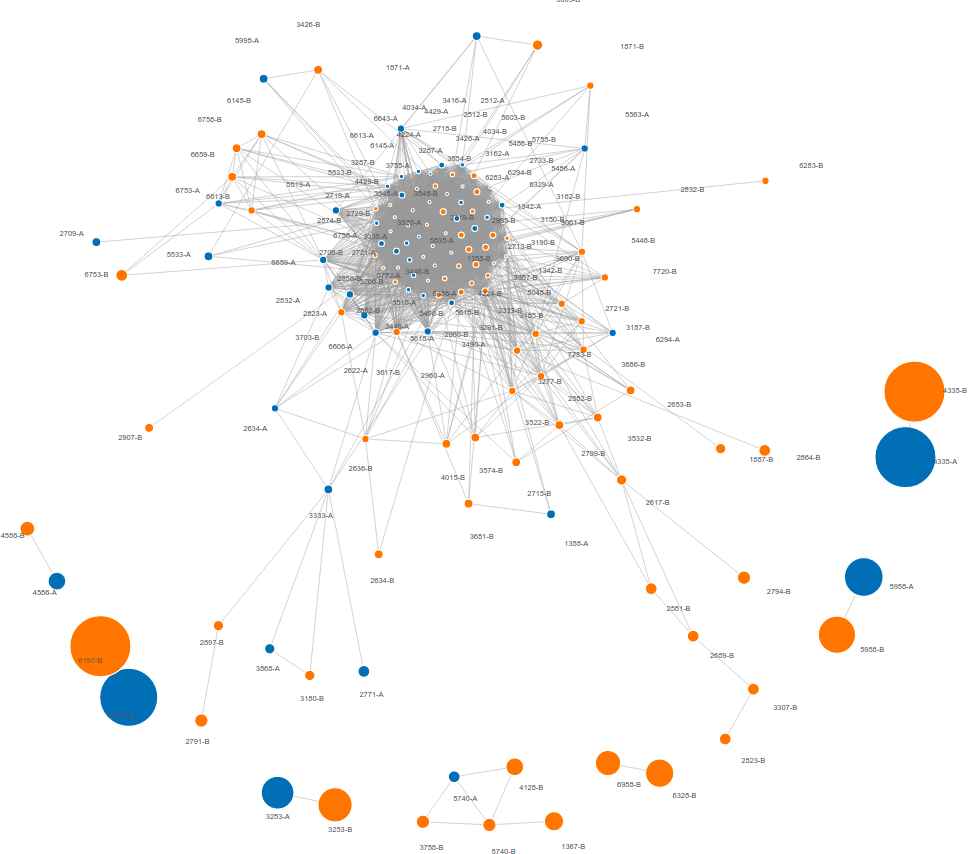
\includegraphics[width=0.9\linewidth]{figures/india.png}
     \caption{\textbf{India DNS censorship}\,---\,%
            We formed clusters of DNS resolvers using the levenshtein distance between
            the lists resolvers censor. Resolvers that block similar lists are connected,
            with node sizes proportional to the number of distinct domains blocked. We color
            IPv4 resolver interfaces blue, and IPv6 interfaces orange. This example illustrates
            the non-uniformity of India, with some ISPs censoring a large number of domains, and
            many others with small or non-existent block lists.}
    \label{fig:india}
    \end{figure}
}

\newcommand{\EveryCountryTable}{
    \begin{table}[ht]
        \centering
        {\tiny\renewcommand{\arraystretch}{.8}
        \resizebox{!}{.35\paperheight}{%
        \begin{tabular}{c|cc}
            \toprule
            \textbf{Country Code} & \textbf{Number of Resolver Pairs} & \textbf{Number of Censored Domains}\\
            \midrule
            US & 1228 & 0\\
            DE & 753 & 1\\
            KR & 632 & 2\\
            FR & 560 & 0\\
            RU & 312 & 33\\
            IR & 277 & 172\\
            VN & 252 & 2\\
            TW & 248 & 2\\
            IN & 226 & 2\\
            CA & 199 & 0\\
            GB & 196 & 0\\
            CN & 194 & 203\\
            TH & 186 & 2\\
            BR & 160 & 2\\
            JP & 152 & 0\\
            MX & 150 & 1\\
            TR & 114 & 3\\
            NL & 97 & 0\\
            ZA & 93 & 2\\
            AU & 72 & 0\\
            HK & 67 & 33\\
            CL & 65 & 2\\
            CH & 60 & 1\\
            ID & 56 & 2\\
            LT & 52 & 3\\
            SG & 50 & 3\\
            MY & 50 & 2\\
            ES & 49 & 0\\
            PL & 48 & 2\\
            AR & 47 & 2\\
            RO & 44 & 2\\
            CZ & 41 & 2\\
            IT & 38 & 1\\
            UA & 35 & 3\\
            SE & 34 & 0\\
            FI & 34 & 0\\
            BE & 31 & 1\\
            BG & 30 & 2\\
            BD & 29 & 3\\
            CO & 27 & 2\\
            SA & 24 & 2\\
            PK & 23 & 2\\
            HU & 22 & 1\\
            EC & 21 & 3\\
            GR & 20 & 0\\
            KZ & 19 & 0\\
            PH & 18 & 3\\
            NO & 16 & 0\\
            SK & 14 & 2\\
            EG & 14 & 17\\
            DK & 13 & 1\\
            PT & 11 & 0\\
            PE & 11 & 3\\
            NG & 9 & 2\\
            KE & 8 & 4\\
            AT & 8 & 1\\
            SI & 7 & 1\\
            RS & 7 & 0\\
            NZ & 7 & 1\\
            NP & 7 & 0\\
            MD & 7 & 0\\
            UY & 6 & 1\\
            MO & 6 & 32\\
            EE & 6 & 0\\
            CR & 6 & 3\\
            AE & 6 & 6\\
            VE & 5 & 2\\
            SD & 5 & 2\\
            PA & 5 & 0\\
            MN & 5 & 0\\
            LY & 5 & 1\\
            BY & 5 & 1\\
            AM & 5 & 1\\
            LV & 4 & 0\\
            LU & 4 & 0\\
            JO & 4 & 0\\
            IQ & 4 & 2\\
            GT & 4 & 0\\
            BZ & 4 & 1\\
            BO & 4 & 1\\
            BA & 4 & 1\\
            AL & 4 & 4\\
            LB & 3 & 1\\
            HR & 3 & 1\\
            HN & 3 & 1\\
            DO & 3 & 1\\
            AF & 3 & 0\\
            UG & 2 & 3\\
            TT & 2 & 0\\
            TN & 2 & 4\\
            TD & 2 & 2\\
            SV & 2 & 0\\
            OM & 2 & 2\\
            NI & 2 & 0\\
            MK & 2 & 49\\
            LA & 2 & 3\\
            IL & 2 & 31\\
            GU & 2 & 2\\
            GE & 2 & 2\\
            ET & 2 & 3\\
            CY & 2 & 3\\
            ZM & 1 & 5\\
            TZ & 1 & 4\\
            TG & 1 & 7\\
            SO & 1 & 1\\
            SC & 1 & 3\\
            PY & 1 & 8\\
            PF & 1 & 2\\
            MZ & 1 & 15\\
            MV & 1 & 11\\
            MM & 1 & 3\\
            MG & 1 & 7\\
            LK & 1 & 1\\
            LI & 1 & 1\\
            LC & 1 & 0\\
            KW & 1 & 1\\
            KG & 1 & 3\\
            HT & 1 & 0\\
            GI & 1 & 5\\
            GH & 1 & 2\\
            FJ & 1 & 2\\
            CM & 1 & 2\\
            AZ & 1 & 1\\
            AO & 1 & 4\\
            AI & 1 & 99\\
            PW & 0 & 3\\
            MA & 0 & 0\\
            KH & 0 & 4\\
            \bottomrule
        \end{tabular}}}
    \end{table}
}

\newcommand{\CompleteCountryTable}{
    \begin{table}[ht]
        \centering
        \begin{adjustbox}{width=\textwidth}
            \begin{tabular}{c|cc|cc|cc}
                \toprule
                \textbf{Country Code} & \textbf{Number of Resolver Pairs (January)} & \textbf{Number of Censored Domains (January)} & \textbf{Number of Resolver Pairs (December)} & \textbf{Number of Censored Domains (December)} & \textbf{Number of Resolver Pairs (November)} & \textbf{Number of Censored Domains (November)}\\
                \midrule
                US & 1228 & 0 & 1189 & 0 & 1201 & 0\\
                DE & 753 & 1 & 721 & 0 & 735 & 0\\
                KR & 632 & 2 & 504 & 2 & 595 & 2\\
                FR & 560 & 0 & 528 & 0 & 542 & 0\\
                RU & 312 & 33 & 296 & 32 & 316 & 33\\
                IR & 277 & 172 & 219 & 120 & 220 & 121\\
                VN & 252 & 2 & 179 & 2 & 214 & 2\\
                TW & 248 & 2 & 201 & 2 & 144 & 2\\
                IN & 226 & 2 & 181 & 2 & 185 & 2\\
                CA & 199 & 0 & 197 & 0 & 205 & 0\\
                GB & 196 & 0 & 196 & 0 & 190 & 0\\
                CN & 194 & 203 & 6 & 32 & 6 & 33\\
                TH & 186 & 2 & 144 & 3 & 202 & 2\\
                BR & 160 & 2 & 146 & 2 & 134 & 2\\
                JP & 152 & 0 & 138 & 0 & 142 & 0\\
                MX & 150 & 1 & 143 & 0 & 90 & 0\\
                TR & 114 & 3 & 90 & 2 & 102 & 2\\
                NL & 97 & 0 & 89 & 0 & 75 & 0\\
                ZA & 93 & 2 & 85 & 2 & 86 & 2\\
                AU & 72 & 0 & 65 & 0 & 71 & 0\\
                HK & 67 & 33 & 57 & 32 & 62 & 33\\
                CL & 65 & 2 & 46 & 2 & 63 & 2\\
                CH & 60 & 1 & 48 & 0 & 51 & 0\\
                ID & 56 & 2 & 31 & 2 & 53 & 2\\
                LT & 52 & 3 & 48 & 2 & 47 & 3\\
                SG & 50 & 3 & 29 & 2 & 39 & 3\\
                MY & 50 & 2 & 34 & 2 & 42 & 2\\
                ES & 49 & 0 & 46 & 0 & 54 & 0\\
                PL & 48 & 2 & 46 & 2 & 46 & 2\\
                AR & 47 & 2 & 47 & 2 & 55 & 2\\
                RO & 44 & 2 & 41 & 2 & 31 & 2\\
                CZ & 41 & 2 & 43 & 2 & 36 & 2\\
                IT & 38 & 1 & 29 & 0 & 31 & 0\\
                UA & 35 & 3 & 33 & 3 & 39 & 3\\
                SE & 34 & 0 & 34 & 0 & 35 & 0\\
                FI & 34 & 0 & 36 & 0 & 32 & 0\\
                BE & 31 & 1 & 32 & 0 & 26 & 0\\
                BG & 30 & 2 & 28 & 2 & 27 & 2\\
                BD & 29 & 3 & 7 & 3 & 21 & 2\\
                CO & 27 & 2 & 20 & 2 & 23 & 2\\
                SA & 24 & 2 & 15 & 2 & 11 & 2\\
                PK & 23 & 2 & 13 & 3 & 10 & 6\\
                HU & 22 & 1 & 16 & 0 & 15 & 1\\
                EC & 21 & 3 & 13 & 1 & 13 & 0\\
                GR & 20 & 0 & 13 & 0 & 15 & 0\\
                KZ & 19 & 0 & 14 & 1 & 21 & 0\\
                PH & 18 & 3 & 24 & 2 & 21 & 2\\
                NO & 16 & 0 & 16 & 0 & 13 & 0\\
                SK & 14 & 2 & 13 & 0 & 11 & 0\\
                EG & 14 & 17 & 13 & 16 & 2 & 27\\
                DK & 13 & 1 & 12 & 0 & 19 & 0\\
                PT & 11 & 0 & 15 & 0 & 11 & 0\\
                PE & 11 & 3 & 10 & 2 & 10 & 2\\
                NG & 9 & 2 & 7 & 3 & 6 & 2\\
                KE & 8 & 4 & 5 & 6 & 5 & 6\\
                AT & 8 & 1 & 11 & 0 & 8 & 1\\
                SI & 7 & 1 & 6 & 0 & 5 & 1\\
                RS & 7 & 0 & 6 & 0 & 4 & 0\\
                NZ & 7 & 1 & 5 & 0 & 6 & 0\\
                NP & 7 & 0 & 3 & 1 & 6 & 0\\
                MD & 7 & 0 & 5 & 0 & 1 & 1\\
                UY & 6 & 1 & 5 & 0 & 6 & 1\\
                MO & 6 & 32 & 7 & 31 & 4 & 31\\
                EE & 6 & 0 & 8 & 0 & 10 & 0\\
                CR & 6 & 3 & 6 & 2 & 4 & 0\\
                AE & 6 & 6 & 3 & 1 & 4 & 5\\
                VE & 5 & 2 & 4 & 2 & 5 & 2\\
                SD & 5 & 2 & 3 & 2 & 2 & 4\\
                PA & 5 & 0 & 3 & 0 & 4 & 0\\
                MN & 5 & 0 & 4 & 1 & 5 & 0\\
                LY & 5 & 1 & 4 & 3 & 5 & 2\\
                BY & 5 & 1 & 5 & 1 & 4 & 1\\
                AM & 5 & 1 & 2 & 5 & 2 & 1\\
                LV & 4 & 0 & 5 & 0 & 3 & 0\\
                LU & 4 & 0 & 3 & 0 & 3 & 0\\
                JO & 4 & 0 & 2 & 0 & 3 & 0\\
                IQ & 4 & 2 & 4 & 0 & 2 & 0\\
                GT & 4 & 0 & 5 & 0 & 6 & 0\\
                BZ & 4 & 1 & 3 & 1 & 2 & 1\\
                BO & 4 & 1 & 5 & 0 & 3 & 0\\
                BA & 4 & 1 & 3 & 1 & 3 & 0\\
                AL & 4 & 4 & 1 & 4 & 4 & 1\\
                LB & 3 & 1 & 2 & 0 & 2 & 0\\
                HR & 3 & 1 & 3 & 0 & 3 & 1\\
                HN & 3 & 1 & 3 & 0 & 1 & 0\\
                DO & 3 & 1 & 2 & 0 & 2 & 0\\
                AF & 3 & 0 & 2 & 3 & 3 & 4\\
                UG & 2 & 3 & 0 & -1 & 1 & 4\\
                TT & 2 & 0 & 2 & 1 & 2 & 0\\
                TN & 2 & 4 & 2 & 1 & 2 & 2\\
                TD & 2 & 2 & 2 & 2 & 2 & 2\\
                SV & 2 & 0 & 1 & 2 & 1 & 1\\
                OM & 2 & 2 & 1 & 2 & 1 & 0\\
                NI & 2 & 0 & 2 & 0 & 2 & 0\\
                MK & 2 & 49 & 1 & 2 & 2 & 50\\
                LA & 2 & 3 & 1 & 4 & 3 & 2\\
                IL & 2 & 31 & 4 & 0 & 4 & 0\\
                GU & 2 & 2 & 2 & 3 & 2 & 2\\
                GE & 2 & 2 & 2 & 3 & 3 & 1\\
                ET & 2 & 3 & 2 & 6 & 2 & 1\\
                CY & 2 & 3 & 2 & 2 & 3 & 3\\
                ZM & 1 & 5 & 0 & -1 & 0 & -1\\
                TZ & 1 & 4 & 1 & 5 & 1 & 7\\
                TG & 1 & 7 & 0 & -1 & 0 & 6\\
                SO & 1 & 1 & 1 & 3 & 1 & 2\\
                SC & 1 & 3 & 2 & 3 & 1 & 4\\
                PY & 1 & 8 & 2 & 7 & 2 & 6\\
                PF & 1 & 2 & 1 & 3 & 1 & 2\\
                MZ & 1 & 15 & 1 & 24 & 0 & -1\\
                MV & 1 & 11 & 0 & -1 & 0 & -1\\
                MM & 1 & 3 & 0 & -1 & 0 & -1\\
                MG & 1 & 7 & 1 & 5 & 2 & 6\\
                LK & 1 & 1 & 1 & 1 & 0 & -1\\
                LI & 1 & 1 & 1 & 1 & 1 & 2\\
                LC & 1 & 0 & 0 & -1 & 1 & 0\\
                KW & 1 & 1 & 1 & 1 & 1 & 1\\
                KG & 1 & 3 & 2 & 4 & 1 & 3\\
                HT & 1 & 0 & 0 & -1 & 0 & -1\\
                GI & 1 & 5 & 1 & 7 & 1 & 3\\
                GH & 1 & 2 & 1 & 2 & 2 & 2\\
                FJ & 1 & 2 & 0 & -1 & 0 & -1\\
                CM & 1 & 2 & 0 & -1 & 0 & -1\\
                AZ & 1 & 1 & 1 & 1 & 1 & 1\\
                AO & 1 & 4 & 1 & 2 & 1 & 3\\
                AI & 1 & 99 & 0 & -1 & 0 & -1\\
                PW & 0 & 3 & 1 & 1 & 1 & 1\\
                MA & 0 & 0 & 0 & 0 & 0 & -1\\
                KH & 0 & 4 & 3 & 2 & 0 & -1\\
                \bottomrule
            \end{tabular}
        \end{adjustbox}
    \end{table}
}



\newcommand{\TabBaseRateAllCountriesMedian}{
    \begin{table}[ht]
        \centering
        \small
        \scalebox{\tabularscale} {
        \begin{tabular}{lccccc}
            \toprule
                %\textbf{Country} & \textbf{Resolver pairs} & \textbf{v4/A} & \textbf{v4/AAAA} & \textbf{v6/A} & \textbf{v6/AAAA} \\
                \textbf{} & \textbf{Resolver} & \textbf{IPv4} & \textbf{IPv4} & \textbf{IPv6} & \textbf{IPv6} \\
                \textbf{Country} & \textbf{pairs} & \textbf{A} & \textbf{AAAA} & \textbf{A} & \textbf{AAAA} \\
                \midrule


Spain (ES)            &    49  & 0.4\% & 0.3\% & 0.1\% & 0.3\% \\  % avg 1.3 stdev 5.5 med 0.3
Poland (PL)           &    48  & 0.7\% & 0.6\% & 0.6\% & 0.4\% \\  % avg 1.7 stdev 5.7 med 0.6
Argentina (AR)        &    47  & 2.4\% & \cellcolor{green1} 0.8\% & \cellcolor{green1} 0.6\% & \cellcolor{green1} 0.4\% \\  % avg 3.0 stdev 4.4 med 0.7
Romania (RO)          &    44  & 0.7\% & \cellcolor{green0} 0.4\% & \cellcolor{green0} 0.4\% & \cellcolor{green0} 0.4\% \\  % avg 1.3 stdev 2.9 med 0.4
Czechia (CZ)          &    41  & 0.4\% & 0.6\% & 0.4\% & 0.6\% \\  % avg 0.9 stdev 2.0 med 0.4
Italy (IT)            &    38  & \cellcolor{green0} 0.7\% & \cellcolor{green0} 0.6\% & \cellcolor{green0} 0.4\% & \cellcolor{green0} 0.6\% \\  % avg 2.3 stdev 5.0 med 0.6
Sweden (SE)           &    34  & 0.1\% & 0.1\% & 0.1\% & 0.1\% \\  % avg 0.4 stdev 1.0 med 0.1
Finland (FI)          &    34  & \cellcolor{green0} 0.4\% & 0.6\% & \cellcolor{green0} 0.4\% & 0.6\% \\  % avg 0.6 stdev 0.4 med 0.6
Ukraine (UA)          &    34  & 3.1\% & \cellcolor{green0} 1.3\% & \cellcolor{green0} 0.8\% & \cellcolor{green0} 1.3\% \\  % avg 3.4 stdev 5.9 med 1.3
Belgium (BE)          &    31  & 0.6\% & \cellcolor{green0} 0.3\% & 0.4\% & \cellcolor{green0} 0.3\% \\  % avg 1.2 stdev 3.5 med 0.3
Bulgaria (BG)         &    30  & \cellcolor{green0} 0.4\% & \cellcolor{green0} 0.4\% & \cellcolor{green0} 0.4\% & \cellcolor{green0} 0.4\% \\  % avg 2.1 stdev 5.9 med 0.4
Bangladesh (BD)       &    29  & \cellcolor{red5}  8.3\% & \cellcolor{green0} 0.6\% & \cellcolor{green0} 0.6\% & \cellcolor{green0} 0.6\% \\  % avg 2.4 stdev 3.7 med 0.7
Colombia (CO)         &    27  & 1.8\% & \cellcolor{green0} 0.7\% & \cellcolor{green0} 0.7\% & \cellcolor{green0} 0.4\% \\  % avg 2.3 stdev 5.6 med 0.7
Saudi Arabia (SA)     &    24  & \cellcolor{green0} 0.7\% & \cellcolor{green0} 0.7\% & \cellcolor{green0} 0.4\% & \cellcolor{green0} 0.7\% \\  % avg 1.8 stdev 4.1 med 0.7
Pakistan (PK)         &    23  & \cellcolor{red1} 4.5\% & \cellcolor{green1} 1.7\% & \cellcolor{red0} 3.8\% & \cellcolor{green1} 1.4\% \\  % avg 3.0 stdev 2.2 med 2.1
Hungary (HU)          &    22  & \cellcolor{green1} 0.1\% & 0.3\% & \cellcolor{green1} 0.1\% & 0.3\% \\  % avg 0.3 stdev 0.3 med 0.3
Ecuador (EC)          &    21  & 1.1\% & 0.4\% & 0.4\% & 0.4\% \\  % avg 1.8 stdev 6.3 med 0.4
Greece (GR)           &    20  & \cellcolor{green0} 0.3\% & \cellcolor{green0} 0.3\% & \cellcolor{green0} 0.3\% & 0.4\% \\  % avg 0.7 stdev 1.4 med 0.3
Kazakhstan (KZ)       &    19  & \cellcolor{green0} 1.0\% & \cellcolor{green0} 0.8\% & \cellcolor{green0} 0.8\% & \cellcolor{green0} 1.0\% \\  % avg 2.4 stdev 4.3 med 0.8
Philippines (PH)      &    18  & 3.4\% & \cellcolor{green0} 1.7\% & \cellcolor{green1} 0.6\% & \cellcolor{green1} 0.6\% \\  % avg 2.8 stdev 4.0 med 1.3
Norway (NO)           &    16  & 0.3\% & \cellcolor{red0} 0.4\% & 0.3\% & \cellcolor{red0} 0.4\% \\  % avg 0.3 stdev 0.3 med 0.3
Egypt (EG)            &    14  & 3.4\% & 3.1\% & \cellcolor{green0} 2.4\% & \cellcolor{green0} 2.8\% \\  % avg 4.1 stdev 4.5 med 2.9
Slovakia (SK)         &    14  & 0.3\% & 0.3\% & 0.3\% & \cellcolor{red2} 0.4\% \\  % avg 0.2 stdev 0.2 med 0.3
Denmark (DK)          &    13  & \cellcolor{green0} 0.4\% & 0.6\% & \cellcolor{green0} 0.3\% & \cellcolor{green0} 0.3\% \\  % avg 1.2 stdev 3.0 med 0.4
Peru (PE)             &    11  & 1.0\% & \cellcolor{green0} 0.6\% & \cellcolor{green0} 0.6\% & \cellcolor{green0} 0.4\% \\  % avg 1.0 stdev 1.5 med 0.6
Portugal (PT)         &    11  & \cellcolor{green0} 0.1\% & \cellcolor{green0} 0.1\% & \cellcolor{green0} 0.0\% & \cellcolor{green0} 0.1\% \\  % avg 0.8 stdev 2.1 med 0.1
Nigeria (NG)          &     9  & 1.7\% & \cellcolor{green1} 0.6\% & 1.7\% & \cellcolor{green0} 1.3\% \\  % avg 2.0 stdev 2.5 med 1.7
Austria (AT)          &     8  & 0.1\% & \cellcolor{red2} 0.3\% & 0.1\% & 0.1\% \\  % avg 0.2 stdev 0.1 med 0.1
Kenya (KE)            &     8  & \cellcolor{red5}  9.9\% & \cellcolor{green0} 1.4\% & \cellcolor{green0} 1.1\% & \cellcolor{green0} 1.1\% \\  % avg 2.8 stdev 4.0 med 1.3
Moldova (MD)          &     7  & \cellcolor{green1} 0.1\% & \cellcolor{green1} 0.3\% & \cellcolor{green1} 0.3\% & \cellcolor{green1} 0.7\% \\  % avg 3.7 stdev 6.0 med 0.3
Serbia (RS)           &     7  & 0.1\% & \cellcolor{red1} 0.3\% & 0.1\% & \cellcolor{red1} 0.3\% \\  % avg 0.2 stdev 0.1 med 0.1
Slovenia (SI)         &     7  & \cellcolor{green0} 0.1\% & \cellcolor{green0} 0.3\% & \cellcolor{green0} 0.1\% & \cellcolor{green0} 0.1\% \\  % avg 1.0 stdev 2.4 med 0.1
New Zealand (NZ)      &     7  & \cellcolor{red5}  6.4\% & \cellcolor{green0} 0.1\% & 0.7\% & \cellcolor{green0} 0.1\% \\  % avg 1.3 stdev 2.5 med 0.1
Nepal (NP)            &     7  & 0.8\% & 0.8\% & \cellcolor{green1} 0.4\% & \cellcolor{green0} 0.7\% \\  % avg 1.0 stdev 0.8 med 0.7
Macao (MO)            &     6  & \cellcolor{green2} 4.3\% & 4.5\% & \cellcolor{green2} 4.3\% & 4.5\% \\  % avg 4.5 stdev 0.2 med 4.5
United Arab Emirates (AE)  &     6  & \cellcolor{red5}  1.7\% & \cellcolor{green1} 0.8\% & \cellcolor{green0} 1.0\% & \cellcolor{green0} 1.0\% \\  % avg 1.1 stdev 0.5 med 1.0
Estonia (EE)          &     6  & 0.6\% & 0.6\% & 0.4\% & 0.6\% \\  % avg 0.7 stdev 1.4 med 0.4
Costa Rica (CR)       &     6  & \cellcolor{red1} 7.3\% & \cellcolor{green0} 0.7\% & \cellcolor{green1} 0.6\% & \cellcolor{green1} 0.4\% \\  % avg 3.8 stdev 6.4 med 0.6
Uruguay (UY)          &     6  & \cellcolor{red1} 0.6\% & 0.4\% & \cellcolor{green0} 0.3\% & \cellcolor{green1} 0.1\% \\  % avg 0.4 stdev 0.3 med 0.3
Libya (LY)            &     5  & \cellcolor{green0} 0.4\% & 0.7\% & \cellcolor{green0} 0.4\% & \cellcolor{green0} 0.4\% \\  % avg 0.8 stdev 0.9 med 0.6
Mongolia (MN)         &     5  & \cellcolor{red0} 1.3\% & 0.8\% & 0.8\% & \cellcolor{green0} 0.7\% \\  % avg 1.0 stdev 0.9 med 0.8
Venezuela (VE)        &     5  & \cellcolor{red5}  8.0\% & \cellcolor{green0} 0.8\% & \cellcolor{green0} 0.7\% & \cellcolor{green0} 0.7\% \\  % avg 2.5 stdev 3.9 med 0.8
Belarus (BY)          &     5  & 0.8\% & \cellcolor{green1} 0.3\% & \cellcolor{green1} 0.3\% & 0.7\% \\  % avg 0.7 stdev 0.7 med 0.4
Armenia (AM)          &     5  & \cellcolor{green1} 0.4\% & \cellcolor{green2} 0.3\% & \cellcolor{green1} 0.4\% & 0.7\% \\  % avg 0.7 stdev 0.6 med 0.4
Panama (PA)           &     5  & 1.7\% & \cellcolor{green0} 0.8\% & \cellcolor{green0} 0.3\% & \cellcolor{green0} 0.3\% \\  % avg 2.1 stdev 4.1 med 0.7
Sudan (SD)            &     5  & 3.1\% & 3.8\% & \cellcolor{green1} 1.3\% & \cellcolor{green1} 1.4\% \\  % avg 3.4 stdev 3.0 med 2.8
Bosnia and Herzegovina (BA)  &     4  & \cellcolor{red1} 2.1\% & \cellcolor{green0} 0.4\% & \cellcolor{green0} 0.4\% & \cellcolor{green0} 0.4\% \\  % avg 1.1 stdev 1.5 med 0.4
Guatemala (GT)        &     4  & 0.4\% & \cellcolor{red0} 0.6\% & \cellcolor{green1} 0.3\% & \cellcolor{green1} 0.3\% \\  % avg 0.4 stdev 0.3 med 0.4
Luxembourg (LU)       &     4  & 0.1\% & 0.1\% & \cellcolor{green0} 0.0\% & 0.1\% \\  % avg 0.6 stdev 1.7 med 0.1
Iraq (IQ)             &     4  & \cellcolor{green0} 1.0\% & \cellcolor{green0} 0.8\% & \cellcolor{green0} 1.0\% & \cellcolor{green0} 1.1\% \\  % avg 2.6 stdev 3.7 med 0.8
Latvia (LV)           &     4  & \cellcolor{green2} 0.0\% & 0.1\% & 0.1\% & 0.1\% \\  % avg 0.1 stdev 0.1 med 0.1
Albania (AL)          &     4  & \cellcolor{green0} 0.4\% & 0.6\% & \cellcolor{green0} 0.4\% & \cellcolor{green0} 0.4\% \\  % avg 0.5 stdev 0.3 med 0.4
Jordan (JO)           &     4  & 0.3\% & 0.3\% & \cellcolor{green1} 0.1\% & \cellcolor{red2} 0.6\% \\  % avg 0.3 stdev 0.3 med 0.3
Belize (BZ)           &     4  & \cellcolor{red5}  8.7\% & \cellcolor{green0} 0.6\% & \cellcolor{green0} 0.6\% & \cellcolor{green0} 0.4\% \\  % avg 1.8 stdev 3.0 med 0.6
Bolivia (BO)          &     4  & 0.6\% & 0.6\% & \cellcolor{green0} 0.3\% & 0.4\% \\  % avg 0.6 stdev 0.7 med 0.4
Croatia (HR)          &     3  & \cellcolor{green1} 0.1\% & \cellcolor{red5}  0.3\% & \cellcolor{green1} 0.1\% & \cellcolor{green1} 0.1\% \\  % avg 0.2 stdev 0.1 med 0.1
Lebanon (LB)          &     3  & \cellcolor{red5}  0.7\% & 0.4\% & 0.4\% & 0.4\% \\  % avg 0.4 stdev 0.2 med 0.4
Afghanistan (AF)      &     3  & \cellcolor{red2} 2.7\% & \cellcolor{green0} 1.4\% & \cellcolor{green0} 1.4\% & 1.5\% \\  % avg 1.8 stdev 1.1 med 1.5
Honduras (HN)         &     3  & 1.3\% & \cellcolor{red1} 1.5\% & \cellcolor{green1} 0.4\% & \cellcolor{green1} 0.4\% \\  % avg 1.1 stdev 0.9 med 1.1
Dominican Republic (DO)  &     3  & \cellcolor{red5}  6.0\% & \cellcolor{green0} 0.6\% & \cellcolor{green1} 0.3\% & \cellcolor{green0} 0.4\% \\  % avg 1.6 stdev 2.3 med 0.6
North Macedonia (MK)  &     2  & \cellcolor{red5}  18.9\% & \cellcolor{red2} 12.6\% & \cellcolor{red0} 9.1\% & \cellcolor{red0} 9.5\% \\  % avg 6.4 stdev 6.8 med 9.1
Georgia (GE)          &     2  & \cellcolor{red2} 2.2\% & \cellcolor{red5}  2.4\% & \cellcolor{red5}  2.7\% & \cellcolor{red1} 1.8\% \\  % avg 1.2 stdev 1.1 med 1.8
Israel (IL)           &     2  & \cellcolor{red5}  5.2\% & \cellcolor{red5}  5.2\% & \cellcolor{red2} 5.0\% & \cellcolor{red5}  5.2\% \\  % avg 2.8 stdev 2.4 med 5.0
Lao People's Democratic Republic (LA)  &     2  & \cellcolor{red5}  9.7\% & \cellcolor{green0} 0.8\% & \cellcolor{green1} 0.4\% & \cellcolor{green1} 0.6\% \\  % avg 2.6 stdev 3.9 med 0.6
El Salvador (SV)      &     2  & \cellcolor{red5}  1.1\% & 0.4\% & \cellcolor{green2} 0.1\% & \cellcolor{green0} 0.3\% \\  % avg 0.4 stdev 0.3 med 0.3
Chad (TD)             &     2  & \cellcolor{red5}  5.5\% & \cellcolor{red0} 2.1\% & 1.3\% & \cellcolor{red0} 2.2\% \\  % avg 1.4 stdev 1.7 med 1.3
Nicaragua (NI)        &     2  & \cellcolor{red5}  7.1\% & \cellcolor{green0} 0.4\% & 0.7\% & \cellcolor{green0} 0.1\% \\  % avg 1.1 stdev 2.3 med 0.4
Uganda (UG)           &     2  & \cellcolor{green0} 0.8\% & \cellcolor{green0} 0.7\% & \cellcolor{green0} 1.0\% & \cellcolor{red5}  13.0\% \\  % avg 2.0 stdev 4.2 med 0.7
Guam (GU)             &     2  & \cellcolor{red5}  8.7\% & \cellcolor{green1} 0.4\% & \cellcolor{green1} 0.0\% & \cellcolor{green1} 0.4\% \\  % avg 2.2 stdev 3.4 med 0.4
Trinidad and Tobago (TT)  &     2  & \cellcolor{red5}  0.6\% & \cellcolor{red2} 0.3\% & 0.1\% & \cellcolor{green2} 0.0\% \\  % avg 0.1 stdev 0.2 med 0.1
Tunisia (TN)          &     2  & \cellcolor{red1} 0.6\% & \cellcolor{red1} 0.6\% & \cellcolor{red1} 0.6\% & \cellcolor{red5}  0.8\% \\  % avg 0.4 stdev 0.2 med 0.6
Ethiopia (ET)         &     2  & \cellcolor{green0} 0.3\% & \cellcolor{green0} 0.7\% & \cellcolor{red5}  51.1\% & \cellcolor{green0} 0.6\% \\  % avg 6.7 stdev 16.8 med 0.4
Oman (OM)             &     2  & \cellcolor{red5}  10.8\% & 1.3\% & \cellcolor{green0} 0.7\% & 1.0\% \\  % avg 1.8 stdev 3.4 med 0.7
Cyprus (CY)           &     2  & \cellcolor{red5}  9.5\% & 1.4\% & \cellcolor{green0} 0.6\% & \cellcolor{green0} 0.6\% \\  % avg 1.6 stdev 3.0 med 0.6
Liechtenstein (LI)    &     1  & \cellcolor{green5}  0.0\% & \cellcolor{green0} 0.1\% & \cellcolor{green0} 0.1\% & \cellcolor{red5}  0.6\% \\  % avg 0.2 stdev 0.2 med 0.1
Madagascar (MG)       &     1  & \cellcolor{red0} 1.1\% & \cellcolor{red5}  1.4\% & \cellcolor{green5}  0.4\% & \cellcolor{red0} 1.1\% \\  % avg 1.0 stdev 0.4 med 1.1
Myanmar (MM)          &     1  & \cellcolor{red5}  0.7\% & \cellcolor{red5}  0.7\% & \cellcolor{green5}  0.3\% & \cellcolor{green5}  0.3\% \\  % avg 0.5 stdev 0.2 med 0.7
Zambia (ZM)           &     1  & \cellcolor{red5}  2.8\% & \cellcolor{green1} 0.8\% & \cellcolor{green1} 0.8\% & \cellcolor{green1} 0.8\% \\  % avg 1.3 stdev 0.8 med 0.8
Kyrgyzstan (KG)       &     1  & \cellcolor{green5}  0.4\% & \cellcolor{red5}  2.7\% & \cellcolor{red2} 2.4\% & \cellcolor{green1} 1.0\% \\  % avg 1.6 stdev 0.9 med 2.4
Ghana (GH)            &     1  & \cellcolor{red5}  8.8\% & \cellcolor{green0} 0.8\% & \cellcolor{green1} 0.1\% & \cellcolor{green1} 0.4\% \\  % avg 2.6 stdev 3.6 med 0.8
Gibraltar (GI)        &     1  & \cellcolor{red5}  1.3\% & \cellcolor{red0} 1.0\% & \cellcolor{green1} 0.7\% & \cellcolor{green5}  0.6\% \\  % avg 0.9 stdev 0.3 med 1.0
Haiti (HT)            &     1  & \cellcolor{red5}  8.5\% & \cellcolor{green1} 0.3\% & \cellcolor{green1} 0.4\% & \cellcolor{green1} 0.0\% \\  % avg 2.3 stdev 3.6 med 0.4
Togo (TG)             &     1  & \cellcolor{red5}  3.9\% & \cellcolor{green0} 1.5\% & \cellcolor{green5}  0.8\% & 1.8\% \\  % avg 2.0 stdev 1.1 med 1.8
Somalia (SO)          &     1  & \cellcolor{red5}  6.0\% & \cellcolor{green1} 0.6\% & \cellcolor{green1} 0.0\% & \cellcolor{green0} 0.7\% \\  % avg 1.8 stdev 2.4 med 0.7
Azerbaijan (AZ)       &     1  & \cellcolor{green1} 0.1\% & \cellcolor{red5}  0.3\% & \cellcolor{green1} 0.1\% & \cellcolor{green1} 0.1\% \\  % avg 0.2 stdev 0.1 med 0.1
Saint Lucia (LC)      &     1  & \cellcolor{green5}  0.0\% & \cellcolor{green5}  0.0\% & \cellcolor{green5}  0.0\% & \cellcolor{green5}  0.0\% \\  % avg 0.0 stdev 0.0 med 0.0
French Polynesia (PF)  &     1  & 0.3\% & \cellcolor{red5}  0.6\% & \cellcolor{green5}  0.0\% & 0.3\% \\  % avg 0.3 stdev 0.2 med 0.3
Kuwait (KW)           &     1  & \cellcolor{green1} 0.1\% & \cellcolor{red5}  1.1\% & \cellcolor{green1} 0.1\% & \cellcolor{green0} 0.3\% \\  % avg 0.4 stdev 0.4 med 0.3
Angola (AO)           &     1  & \cellcolor{red5}  6.7\% & \cellcolor{green0} 1.0\% & \cellcolor{green1} 0.3\% & \cellcolor{green1} 0.6\% \\  % avg 2.1 stdev 2.7 med 1.0
Maldives (MV)         &     1  & \cellcolor{red5}  8.3\% & \cellcolor{green5}  1.1\% & 5.3\% & \cellcolor{red1} 6.7\% \\  % avg 5.4 stdev 2.7 med 6.7
Fiji (FJ)             &     1  & \cellcolor{red5}  0.4\% & 0.3\% & \cellcolor{green5}  0.1\% & 0.3\% \\  % avg 0.3 stdev 0.1 med 0.3
Mozambique (MZ)       &     1  & \cellcolor{red5}  11.2\% & \cellcolor{green0} 3.8\% & \cellcolor{green1} 3.2\% & \cellcolor{green1} 2.8\% \\  % avg 5.3 stdev 3.5 med 3.8
Sri Lanka (LK)        &     1  & 0.3\% & \cellcolor{red5}  0.8\% & \cellcolor{green1} 0.1\% & \cellcolor{green1} 0.1\% \\  % avg 0.4 stdev 0.3 med 0.3
Paraguay (PY)         &     1  & \cellcolor{red5}  1.5\% & \cellcolor{green0} 1.1\% & \cellcolor{green5}  1.0\% & \cellcolor{green0} 1.1\% \\  % avg 1.2 stdev 0.2 med 1.1
Seychelles (SC)       &     1  & \cellcolor{green1} 0.4\% & \cellcolor{green1} 0.4\% & \cellcolor{red5}  0.6\% & \cellcolor{green1} 0.4\% \\  % avg 0.5 stdev 0.1 med 0.4
Tanzania (TZ)         &     1  & \cellcolor{red5}  7.3\% & 2.5\% & \cellcolor{green2} 0.6\% & \cellcolor{green2} 0.7\% \\  % avg 2.8 stdev 2.7 med 2.5
Cameroon (CM)         &     1  & \cellcolor{green5}  0.1\% & 0.3\% & 0.3\% & \cellcolor{red5}  0.4\% \\  % avg 0.3 stdev 0.1 med 0.3
Anguilla (AI)         &     1  & \cellcolor{red5}  25.9\% & \cellcolor{green0} 12.7\% & \cellcolor{green1} 11.1\% & \cellcolor{green2} 9.8\% \\  % avg 14.9 stdev 6.5 med 12.7
\hline
\textbf{Global}            & \textbf{ 7441} & \textbf{3.6\%} & \textbf{3.0\%} & \textbf{2.6\%} & \textbf{2.7\%} \\ % avg 3.0 stdev 7.0 med 0.4
                \bottomrule
        \end{tabular}
        }
        \caption{\textbf{Base rate medians; rest of countries not included in Table~\ref{tab:base-rate}}}
    \end{table}
}
 



\newcommand{\TabBaseRateAllCountries}{
    \begin{table}[ht]
        \centering
        \small
        \scalebox{\tabularscale} {
        \begin{tabular}{lccccc}
            \toprule
                %\textbf{Country} & \textbf{Resolver pairs} & \textbf{v4/A} & \textbf{v4/AAAA} & \textbf{v6/A} & \textbf{v6/AAAA} \\
                \textbf{} & \textbf{Resolver} & \textbf{IPv4} & \textbf{IPv4} & \textbf{IPv6} & \textbf{IPv6} \\
                \textbf{Country} & \textbf{pairs} & \textbf{A} & \textbf{AAAA} & \textbf{A} & \textbf{AAAA} \\
                \midrule


Spain (ES)            &    49  & 0.9\% & 0.8\% & 1.4\% & 2.0\% \\  % avg 1.3 stdev 5.5 med 0.3
Poland (PL)           &    48  & 2.0\% & 1.1\% & 2.9\% & 1.0\% \\  % avg 1.7 stdev 5.7 med 0.6
Argentina (AR)        &    47  & \cellcolor{red0} 5.2\% & 3.5\% & 2.2\% & \cellcolor{green0} 1.3\% \\  % avg 3.0 stdev 4.4 med 0.7
Romania (RO)          &    44  & \cellcolor{red0} 2.3\% & 1.0\% & 0.8\% & 0.9\% \\  % avg 1.3 stdev 2.9 med 0.4
Czechia (CZ)          &    41  & \cellcolor{red0} 1.6\% & 1.1\% & 0.5\% & 0.5\% \\  % avg 0.9 stdev 2.0 med 0.4
Italy (IT)            &    38  & 2.4\% & 2.1\% & 2.2\% & 2.5\% \\  % avg 2.3 stdev 5.0 med 0.6
Sweden (SE)           &    34  & 0.4\% & 0.3\% & 0.5\% & 0.2\% \\  % avg 0.4 stdev 1.0 med 0.1
Finland (FI)          &    34  & \cellcolor{red0} 0.7\% & 0.6\% & \cellcolor{green0} 0.4\% & 0.5\% \\  % avg 0.6 stdev 0.4 med 0.6
Ukraine (UA)          &    34  & \cellcolor{red0} 6.0\% & 2.7\% & 2.4\% & 2.7\% \\  % avg 3.4 stdev 5.9 med 1.3
Belgium (BE)          &    31  & 1.6\% & 1.3\% & 0.9\% & 1.0\% \\  % avg 1.2 stdev 3.5 med 0.3
Bulgaria (BG)         &    30  & 3.2\% & 2.9\% & 1.1\% & 1.1\% \\  % avg 2.1 stdev 5.9 med 0.4
Bangladesh (BD)       &    29  & \cellcolor{red5}  6.4\% & \cellcolor{green0} 1.3\% & \cellcolor{green0} 0.9\% & \cellcolor{green0} 0.8\% \\  % avg 2.4 stdev 3.7 med 0.7
Colombia (CO)         &    27  & 3.4\% & 3.3\% & 1.4\% & 1.1\% \\  % avg 2.3 stdev 5.6 med 0.7
Saudi Arabia (SA)     &    24  & 2.2\% & 1.8\% & 1.6\% & 1.6\% \\  % avg 1.8 stdev 4.1 med 0.7
Pakistan (PK)         &    23  & \cellcolor{red0} 3.7\% & \cellcolor{green1} 1.6\% & \cellcolor{red1} 4.6\% & \cellcolor{green0} 1.9\% \\  % avg 3.0 stdev 2.2 med 2.1
Hungary (HU)          &    22  & 0.3\% & 0.3\% & 0.2\% & 0.3\% \\  % avg 0.3 stdev 0.3 med 0.3
Ecuador (EC)          &    21  & 3.3\% & 2.9\% & 0.4\% & 0.8\% \\  % avg 1.8 stdev 6.3 med 0.4
Greece (GR)           &    20  & 0.5\% & \cellcolor{red0} 1.2\% & 0.4\% & 0.6\% \\  % avg 0.7 stdev 1.4 med 0.3
Kazakhstan (KZ)       &    19  & 2.9\% & 2.0\% & 2.4\% & 2.3\% \\  % avg 2.4 stdev 4.3 med 0.8
Philippines (PH)      &    18  & \cellcolor{red0} 4.3\% & 2.4\% & 2.5\% & 2.0\% \\  % avg 2.8 stdev 4.0 med 1.3
Norway (NO)           &    16  & 0.3\% & 0.3\% & 0.3\% & \cellcolor{red0} 0.4\% \\  % avg 0.3 stdev 0.3 med 0.3
Egypt (EG)            &    14  & \cellcolor{red0} 5.6\% & 4.2\% & 3.1\% & 3.5\% \\  % avg 4.1 stdev 4.5 med 2.9
Slovakia (SK)         &    14  & 0.2\% & 0.3\% & 0.2\% & 0.3\% \\  % avg 0.2 stdev 0.2 med 0.3
Denmark (DK)          &    13  & 1.7\% & 1.3\% & 0.9\% & 1.0\% \\  % avg 1.2 stdev 3.0 med 0.4
Peru (PE)             &    11  & \cellcolor{red1} 2.0\% & 0.8\% & 0.7\% & \cellcolor{green0} 0.6\% \\  % avg 1.0 stdev 1.5 med 0.6
Portugal (PT)         &    11  & \cellcolor{red1} 2.2\% & 0.4\% & \cellcolor{green0} 0.2\% & 0.3\% \\  % avg 0.8 stdev 2.1 med 0.1
Nigeria (NG)          &     9  & \cellcolor{red1} 3.4\% & 1.4\% & 1.6\% & 1.4\% \\  % avg 2.0 stdev 2.5 med 1.7
Austria (AT)          &     8  & \cellcolor{green0} 0.1\% & \cellcolor{red1} 0.2\% & \cellcolor{green1} 0.1\% & \cellcolor{red0} 0.2\% \\  % avg 0.2 stdev 0.1 med 0.1
Kenya (KE)            &     8  & \cellcolor{red5}  7.8\% & \cellcolor{green0} 1.4\% & \cellcolor{green0} 1.1\% & \cellcolor{green0} 1.1\% \\  % avg 2.8 stdev 4.0 med 1.3
Moldova (MD)          &     7  & \cellcolor{red0} 5.5\% & 3.6\% & 2.9\% & 3.0\% \\  % avg 3.7 stdev 6.0 med 0.3
Serbia (RS)           &     7  & 0.2\% & 0.2\% & 0.1\% & 0.2\% \\  % avg 0.2 stdev 0.1 med 0.1
Slovenia (SI)         &     7  & \cellcolor{red5}  3.5\% & \cellcolor{green0} 0.3\% & \cellcolor{green0} 0.1\% & \cellcolor{green0} 0.2\% \\  % avg 1.0 stdev 2.4 med 0.1
New Zealand (NZ)      &     7  & \cellcolor{red5}  4.3\% & \cellcolor{green0} 0.2\% & \cellcolor{green0} 0.5\% & \cellcolor{green0} 0.2\% \\  % avg 1.3 stdev 2.5 med 0.1
Nepal (NP)            &     7  & 1.1\% & 1.2\% & \cellcolor{green0} 0.8\% & 1.0\% \\  % avg 1.0 stdev 0.8 med 0.7
Macao (MO)            &     6  & 4.4\% & 4.5\% & 4.4\% & \cellcolor{red0} 4.5\% \\  % avg 4.5 stdev 0.2 med 4.5
United Arab Emirates (AE)  &     6  & \cellcolor{red5}  1.6\% & \cellcolor{green1} 0.9\% & 1.1\% & \cellcolor{green1} 0.9\% \\  % avg 1.1 stdev 0.5 med 1.0
Estonia (EE)          &     6  & \cellcolor{red1} 1.6\% & 0.4\% & \cellcolor{green0} 0.3\% & 0.4\% \\  % avg 0.7 stdev 1.4 med 0.4
Costa Rica (CR)       &     6  & \cellcolor{red1} 8.6\% & 2.5\% & \cellcolor{green0} 2.2\% & \cellcolor{green0} 2.1\% \\  % avg 3.8 stdev 6.4 med 0.6
Uruguay (UY)          &     6  & \cellcolor{red2} 0.7\% & 0.4\% & \cellcolor{green0} 0.2\% & \cellcolor{green1} 0.2\% \\  % avg 0.4 stdev 0.3 med 0.3
Libya (LY)            &     5  & \cellcolor{red1} 1.4\% & 0.8\% & \cellcolor{green0} 0.4\% & \cellcolor{green0} 0.4\% \\  % avg 0.8 stdev 0.9 med 0.6
Mongolia (MN)         &     5  & \cellcolor{red2} 1.9\% & \cellcolor{green0} 0.7\% & \cellcolor{green0} 0.6\% & \cellcolor{green0} 0.7\% \\  % avg 1.0 stdev 0.9 med 0.8
Venezuela (VE)        &     5  & \cellcolor{red5}  6.7\% & 1.6\% & \cellcolor{green0} 0.8\% & \cellcolor{green0} 0.7\% \\  % avg 2.5 stdev 3.9 med 0.8
Belarus (BY)          &     5  & \cellcolor{red0} 1.0\% & 0.7\% & \cellcolor{green0} 0.4\% & 0.6\% \\  % avg 0.7 stdev 0.7 med 0.4
Armenia (AM)          &     5  & \cellcolor{red0} 0.9\% & 0.6\% & 0.6\% & 0.7\% \\  % avg 0.7 stdev 0.6 med 0.4
Panama (PA)           &     5  & \cellcolor{red0} 3.8\% & \cellcolor{red0} 4.0\% & \cellcolor{green0} 0.3\% & \cellcolor{green0} 0.4\% \\  % avg 2.1 stdev 4.1 med 0.7
Sudan (SD)            &     5  & \cellcolor{red0} 4.6\% & \cellcolor{red0} 4.5\% & \cellcolor{green0} 2.4\% & \cellcolor{green0} 2.3\% \\  % avg 3.4 stdev 3.0 med 2.8
Bosnia and Herzegovina (BA)  &     4  & \cellcolor{red2} 2.2\% & 0.7\% & \cellcolor{green0} 0.6\% & 0.7\% \\  % avg 1.1 stdev 1.5 med 0.4
Guatemala (GT)        &     4  & \cellcolor{red1} 0.6\% & \cellcolor{red0} 0.6\% & 0.4\% & \cellcolor{green2} 0.2\% \\  % avg 0.4 stdev 0.3 med 0.4
Luxembourg (LU)       &     4  & \cellcolor{red2} 1.9\% & \cellcolor{green0} 0.1\% & \cellcolor{green0} 0.1\% & 0.2\% \\  % avg 0.6 stdev 1.7 med 0.1
Iraq (IQ)             &     4  & \cellcolor{red0} 3.6\% & 2.5\% & 2.1\% & 2.1\% \\  % avg 2.6 stdev 3.7 med 0.8
Latvia (LV)           &     4  & 0.1\% & 0.1\% & 0.1\% & 0.1\% \\  % avg 0.1 stdev 0.1 med 0.1
Albania (AL)          &     4  & \cellcolor{red1} 0.7\% & 0.6\% & \cellcolor{green0} 0.4\% & \cellcolor{green0} 0.4\% \\  % avg 0.5 stdev 0.3 med 0.4
Jordan (JO)           &     4  & 0.3\% & 0.2\% & \cellcolor{green1} 0.1\% & \cellcolor{red1} 0.5\% \\  % avg 0.3 stdev 0.3 med 0.3
Belize (BZ)           &     4  & \cellcolor{red5}  5.9\% & \cellcolor{green0} 0.5\% & \cellcolor{green0} 0.4\% & \cellcolor{green0} 0.4\% \\  % avg 1.8 stdev 3.0 med 0.6
Bolivia (BO)          &     4  & \cellcolor{red2} 1.2\% & 0.5\% & \cellcolor{green0} 0.3\% & \cellcolor{green0} 0.3\% \\  % avg 0.6 stdev 0.7 med 0.4
Croatia (HR)          &     3  & \cellcolor{green1} 0.1\% & \cellcolor{red2} 0.2\% & 0.2\% & \cellcolor{green1} 0.1\% \\  % avg 0.2 stdev 0.1 med 0.1
Lebanon (LB)          &     3  & \cellcolor{red5}  0.6\% & 0.4\% & \cellcolor{green1} 0.3\% & 0.4\% \\  % avg 0.4 stdev 0.2 med 0.4
Afghanistan (AF)      &     3  & \cellcolor{red0} 2.2\% & \cellcolor{green1} 1.1\% & 1.9\% & 1.8\% \\  % avg 1.8 stdev 1.1 med 1.5
Honduras (HN)         &     3  & \cellcolor{red0} 1.5\% & \cellcolor{red0} 1.4\% & \cellcolor{green0} 0.7\% & \cellcolor{green0} 0.6\% \\  % avg 1.1 stdev 0.9 med 1.1
Dominican Republic (DO)  &     3  & \cellcolor{red5}  4.8\% & \cellcolor{green0} 0.7\% & \cellcolor{green1} 0.3\% & \cellcolor{green0} 0.5\% \\  % avg 1.6 stdev 2.3 med 0.6

                \bottomrule
        \end{tabular}

        \begin{tabular}{lccccc}
            \toprule
                %\textbf{Country} & \textbf{Resolver pairs} & \textbf{v4/A} & \textbf{v4/AAAA} & \textbf{v6/A} & \textbf{v6/AAAA} \\
                \textbf{} & \textbf{Resolver} & \textbf{IPv4} & \textbf{IPv4} & \textbf{IPv6} & \textbf{IPv6} \\
                \textbf{Country} & \textbf{pairs} & \textbf{A} & \textbf{AAAA} & \textbf{A} & \textbf{AAAA} \\
                \midrule

North Macedonia (MK)  &     2  & \cellcolor{red0} 9.5\% & 6.4\% & 4.7\% & 4.8\% \\  % avg 6.4 stdev 6.8 med 9.1
Georgia (GE)          &     2  & 1.2\% & 1.3\% & 1.4\% & 1.0\% \\  % avg 1.2 stdev 1.1 med 1.8
Israel (IL)           &     2  & 2.7\% & 2.9\% & 2.7\% & 2.7\% \\  % avg 2.8 stdev 2.4 med 5.0
Lao People's Democratic Republic (LA)  &     2  & \cellcolor{red5}  9.2\% & \cellcolor{green1} 0.6\% & \cellcolor{green1} 0.2\% & \cellcolor{green1} 0.3\% \\  % avg 2.6 stdev 3.9 med 0.6
El Salvador (SV)      &     2  & \cellcolor{red5}  0.8\% & 0.4\% & \cellcolor{green2} 0.1\% & \cellcolor{green1} 0.2\% \\  % avg 0.4 stdev 0.3 med 0.3
Chad (TD)             &     2  & \cellcolor{red1} 2.7\% & 1.1\% & \cellcolor{green0} 0.6\% & 1.3\% \\  % avg 1.4 stdev 1.7 med 1.3
Nicaragua (NI)        &     2  & \cellcolor{red5}  3.8\% & \cellcolor{green0} 0.3\% & \cellcolor{green0} 0.4\% & \cellcolor{green0} 0.1\% \\  % avg 1.1 stdev 2.3 med 0.4
Uganda (UG)           &     2  & \cellcolor{green0} 0.5\% & \cellcolor{green0} 0.5\% & \cellcolor{green0} 0.6\% & \cellcolor{red5}  6.7\% \\  % avg 2.0 stdev 4.2 med 0.7
Guam (GU)             &     2  & \cellcolor{red5}  8.1\% & \cellcolor{green1} 0.4\% & \cellcolor{green1} 0.0\% & \cellcolor{green1} 0.4\% \\  % avg 2.2 stdev 3.4 med 0.4
Trinidad and Tobago (TT)  &     2  & \cellcolor{red5}  0.4\% & 0.1\% & \cellcolor{green0} 0.1\% & \cellcolor{green2} 0.0\% \\  % avg 0.1 stdev 0.2 med 0.1
Tunisia (TN)          &     2  & \cellcolor{green0} 0.4\% & 0.4\% & \cellcolor{green0} 0.4\% & \cellcolor{red1} 0.6\% \\  % avg 0.4 stdev 0.2 med 0.6
Ethiopia (ET)         &     2  & \cellcolor{green0} 0.1\% & \cellcolor{green0} 0.6\% & \cellcolor{red5}  25.6\% & \cellcolor{green0} 0.4\% \\  % avg 6.7 stdev 16.8 med 0.4
Oman (OM)             &     2  & \cellcolor{red5}  5.5\% & \cellcolor{green0} 0.7\% & \cellcolor{green0} 0.4\% & \cellcolor{green0} 0.7\% \\  % avg 1.8 stdev 3.4 med 0.7
Cyprus (CY)           &     2  & \cellcolor{red5}  4.8\% & \cellcolor{green0} 0.8\% & \cellcolor{green0} 0.4\% & \cellcolor{green0} 0.3\% \\  % avg 1.6 stdev 3.0 med 0.6
Liechtenstein (LI)    &     1  & \cellcolor{green5}  0.0\% & \cellcolor{green0} 0.1\% & \cellcolor{green0} 0.1\% & \cellcolor{red5}  0.6\% \\  % avg 0.2 stdev 0.2 med 0.1
Madagascar (MG)       &     1  & \cellcolor{red0} 1.1\% & \cellcolor{red5}  1.4\% & \cellcolor{green5}  0.4\% & \cellcolor{red0} 1.1\% \\  % avg 1.0 stdev 0.4 med 1.1
Myanmar (MM)          &     1  & \cellcolor{red5}  0.7\% & \cellcolor{red5}  0.7\% & \cellcolor{green5}  0.3\% & \cellcolor{green5}  0.3\% \\  % avg 0.5 stdev 0.2 med 0.7
Zambia (ZM)           &     1  & \cellcolor{red5}  2.8\% & \cellcolor{green1} 0.8\% & \cellcolor{green1} 0.8\% & \cellcolor{green1} 0.8\% \\  % avg 1.3 stdev 0.8 med 0.8
Kyrgyzstan (KG)       &     1  & \cellcolor{green5}  0.4\% & \cellcolor{red5}  2.7\% & \cellcolor{red2} 2.4\% & \cellcolor{green1} 1.0\% \\  % avg 1.6 stdev 0.9 med 2.4
Ghana (GH)            &     1  & \cellcolor{red5}  8.8\% & \cellcolor{green0} 0.8\% & \cellcolor{green1} 0.1\% & \cellcolor{green1} 0.4\% \\  % avg 2.6 stdev 3.6 med 0.8
Gibraltar (GI)        &     1  & \cellcolor{red5}  1.3\% & \cellcolor{red0} 1.0\% & \cellcolor{green1} 0.7\% & \cellcolor{green5}  0.6\% \\  % avg 0.9 stdev 0.3 med 1.0
Haiti (HT)            &     1  & \cellcolor{red5}  8.5\% & \cellcolor{green1} 0.3\% & \cellcolor{green1} 0.4\% & \cellcolor{green1} 0.0\% \\  % avg 2.3 stdev 3.6 med 0.4
Togo (TG)             &     1  & \cellcolor{red5}  3.9\% & \cellcolor{green0} 1.5\% & \cellcolor{green5}  0.8\% & 1.8\% \\  % avg 2.0 stdev 1.1 med 1.8
Somalia (SO)          &     1  & \cellcolor{red5}  6.0\% & \cellcolor{green1} 0.6\% & \cellcolor{green1} 0.0\% & \cellcolor{green0} 0.7\% \\  % avg 1.8 stdev 2.4 med 0.7
Azerbaijan (AZ)       &     1  & \cellcolor{green1} 0.1\% & \cellcolor{red5}  0.3\% & \cellcolor{green1} 0.1\% & \cellcolor{green1} 0.1\% \\  % avg 0.2 stdev 0.1 med 0.1
Saint Lucia (LC)      &     1  & 0.0\% & 0.0\% & 0.0\% & 0.0\% \\  % avg 0.0 stdev 0.0 med 0.0
French Polynesia (PF)  &     1  & 0.3\% & \cellcolor{red5}  0.6\% & \cellcolor{green5}  0.0\% & 0.3\% \\  % avg 0.3 stdev 0.2 med 0.3
Kuwait (KW)           &     1  & \cellcolor{green1} 0.1\% & \cellcolor{red5}  1.1\% & \cellcolor{green1} 0.1\% & \cellcolor{green0} 0.3\% \\  % avg 0.4 stdev 0.4 med 0.3
Angola (AO)           &     1  & \cellcolor{red5}  6.7\% & \cellcolor{green0} 1.0\% & \cellcolor{green1} 0.3\% & \cellcolor{green1} 0.6\% \\  % avg 2.1 stdev 2.7 med 1.0
Maldives (MV)         &     1  & \cellcolor{red5}  8.3\% & \cellcolor{green5}  1.1\% & 5.3\% & \cellcolor{red1} 6.7\% \\  % avg 5.4 stdev 2.7 med 6.7
Fiji (FJ)             &     1  & \cellcolor{red5}  0.4\% & 0.3\% & \cellcolor{green5}  0.1\% & 0.3\% \\  % avg 0.3 stdev 0.1 med 0.3
Mozambique (MZ)       &     1  & \cellcolor{red5}  11.2\% & \cellcolor{green0} 3.8\% & \cellcolor{green1} 3.2\% & \cellcolor{green1} 2.8\% \\  % avg 5.3 stdev 3.5 med 3.8
Sri Lanka (LK)        &     1  & 0.3\% & \cellcolor{red5}  0.8\% & \cellcolor{green1} 0.1\% & \cellcolor{green1} 0.1\% \\  % avg 0.4 stdev 0.3 med 0.3
Paraguay (PY)         &     1  & \cellcolor{red5}  1.5\% & \cellcolor{green0} 1.1\% & \cellcolor{green5}  1.0\% & \cellcolor{green0} 1.1\% \\  % avg 1.2 stdev 0.2 med 1.1
Seychelles (SC)       &     1  & \cellcolor{green1} 0.4\% & \cellcolor{green1} 0.4\% & \cellcolor{red5}  0.6\% & \cellcolor{green1} 0.4\% \\  % avg 0.5 stdev 0.1 med 0.4
Tanzania (TZ)         &     1  & \cellcolor{red5}  7.3\% & 2.5\% & \cellcolor{green2} 0.6\% & \cellcolor{green2} 0.7\% \\  % avg 2.8 stdev 2.7 med 2.5
Cameroon (CM)         &     1  & \cellcolor{green5}  0.1\% & 0.3\% & 0.3\% & \cellcolor{red5}  0.4\% \\  % avg 0.3 stdev 0.1 med 0.3
Anguilla (AI)         &     1  & \cellcolor{red5}  25.9\% & \cellcolor{green0} 12.7\% & \cellcolor{green1} 11.1\% & \cellcolor{green2} 9.8\% \\  % avg 14.9 stdev 6.5 med 12.7
\hline
\textbf{Global}            & \textbf{ 7441} & \textbf{3.6\%} & \textbf{3.0\%} & \textbf{2.6\%} & \textbf{2.7\%} \\ % avg 3.0 stdev 7.0 med 0.4


        \bottomrule
        \end{tabular}
        }



        \caption{\textbf{Base rate; rest of countries not included in Table~\ref{tab:base-rate}}}
    \end{table}
}

\newcommand{\FigDNSCensorship}{
    \begin{figure}[h!]
        \centering
        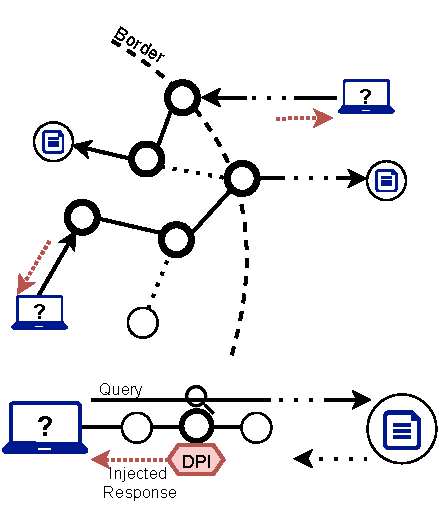
\includegraphics[width=0.8\linewidth]{figures/dns_censorship.pdf}
        \caption{DNS censorship is carried out by on-path or in-path deep packet
        inspection (DPI) appliances that monitor for block-listed keywords or
        expressions in DNS queries and inject forged responses. The original
        request and subsequent response are not typically dropped by the
        adversary, but will arrive after the forged response rendering them
        useless. DPI appliances can be deployed in local infrastructure,
        regional ISPs, or national border gateways and inject the forged response
        toward the query source in either direction.}
        \label{fig:dns_censorship}
      \end{figure}

}


%%% Local Variables:
%%% mode: latex
%%% TeX-master: "main"
%%% End:



\begin{document}

% \renewcommand\footnotetextcopyrightpermission[1]{} % removes footnote with conference information in first column
\pagestyle{plain} % removes running headers


\renewcommand{\sectionautorefname}{\S}
\renewcommand{\subsectionautorefname}{\S}
\renewcommand{\subsubsectionautorefname}{\S}
\date{}

\setlength{\droptitle}{-5em}   % Eliminate vertical space above title
\posttitle{\par\end{center}}   % tighten space between title and author block
\title{{\bf Mind the IP Gap}\\\Large{Measuring the impact of IPv6 on DNS censorship}}
        %On the IPv6 Transition and the Emergence of
%DNS Censorship Inconsistencies}}
\author{Paper \#474}
%for single author (just remove % characters)
% \author{
% {\rm Your N.\ Here}\\
% Your Institution
% \and
% {\rm Second Name}\\
% Second Institution
% copy the following lines to add more authors
% \and
% {\rm Name}\\
%Name Institution
% } % end author


\maketitle

\begin{abstract}
 
Internet censorship continues to impact billions of people worldwide,
and measurement of it remains an important focus of research.
However, most Internet censorship measurements have focused solely on the IPv4
Internet infrastructure. Yet, more clients and servers are available over IPv6:
According to Google, over a third of their users now have native IPv6 access.
% https://www.google.com/intl/en/ipv6/statistics.html

Given the slow-but-steady rate of IPv6 adoption, it is important to understand
its impact on censorship. In this paper, we measure and analyze how censorship
differs over IPv6 compared to the well-studied IPv4 censorship systems in use
today.

We perform a comprehensive global study of censorship across an array of
commonly censored protocols, including HTTP, DNS, TLS, and QUIC, on both IPv4
and IPv6, and compare the results.
% TODO correct this list
We find that there are several differences in how countries censor IPv6 traffic,
both in terms of IPv6 resources, and in where and what blocklists or technology
are deployed on IPv6 networks. Many of these differences are
not all-or-nothing: we find that most censors have some capacity to block
in IPv6, but are less comprehensive or less reliable compared to their IPv4
censorship systems.

Our results suggest that IPv6 offers new areas for censorship circumvention
researchers to explore, providing potentially new ways to evade censors. As more
users gain access to IPv6 addresses and networks, there will be a need for tools
that take advantage of IPv6 techniques and infrastructure to bypass censorship.



\if0
 internet today, as such
it is extremely important to find ways to measure censorship techniques that impart
minimal risk to censored netizens. One of the lowest risk strategies for measuring
censorship relies on censors displaying censorship behavior bidirectionally -
injecting uniformly for inress and egress traffic. However, no comprehensive
study has been done to determine which networks present bidirectional censorship
in IPv4 and IPv6 across protocols known to be censored. This leaves a gap in the
research understanding of where low risk measurement strategies can be
consistently applied.

In this paper we perform a comprehensive global study of bidirectional
censorship across an array of commonly censored protocols. Using a custom tool
to rapidly inject packets and a novel strategy in which we target non-responsive
hosts with probes we trigger bidirectional censorship behavior from
\red{XXX} unique ASNs in \red{N} countries across 4 protocols.

Further we observe that while nearly all censors support blocking IPv6, their
policies are inconsistent with and frequently less effective than their IPv4
censorship infrastructure. Our results suggest that supporting IPv6 censorship
is not all-or-nothing: many censors support it, but poorly.  As a result, these
censors may have to expend additional resources to bring IPv6 censorship up to
parity with IPv4. In the meantime, this affords censorship circumvention
researchers a new opportunity to exploit these differences to evade detection
and blocking.
\fi

\end{abstract}

\section{Introduction}\label{sec:intro}


Internet censorship is a global problem that affects over half the world's
population. Censors rely on sophisticated network middleboxes to inspect and
block traffic, employing IP-based blocking and packet injection to prevent
access to censored content and resources. A common technique used by censors involves
inspecting network traffic
passively, and injecting (spoofed) responses to DNS, TLS, HTTP, or other protocol
requests for censored
content~\cite{lowe2007great,hoang2021great,vandersloot2018quack,xu2011internet,aryan2013internet,chai2019importance,elmenhorst2021web}.


Prior work has extensively studied this type of censorship
globally~\cite{niaki2020iclab,sundara2020censored,filasto2012ooni,razaghpanah2016exploring,kuhrer2015going,dagon2008corrupted,pearce2017global,scott2016satellite}
%
and for individual
countries~\cite{Anonymous2020:TripletCensors,USESEC21:GFWatch,aryan2013internet,ramesh2020decentralized,yadav2018light,gebhart2017internet,nabi2013anatomy}.
%TODO: add other studies that are measuring any kind of injection, not just DNS
%
%\cite{kuhrer2015going,Anonymous2020:TripletCensors,USESEC21:GFWatch,dagon2008corrupted,pearce2017global,scott2016satellite}.
These studies generally perform active measurements that test large
%of DNS resolvers for large
sets of domains in requests into censored countries, and identify forged
censorship responses from legitimate ones.
%
Unfortunately, this prior work has focused exclusively on the IPv4 Internet, in
part because scanning the IPv6 Internet for servers is
difficult~\cite{murdock2017target}, owing to its impossible-to-enumerate 128-bit
address space.
%

An IPv4-only view of censorship is problematic, because
IPv6 is becoming more widely deployed and used worldwide: over 35\% of current Internet
traffic is being served over native IPv6 connections~\cite{Google-IPv6} (and exceeds
50\% in some countries known to censor such as India~\cite{akamai-ipv6}).
However, it
is unclear if the same censorship mechanisms we know about in IPv4 traffic
also apply to the growing IPv6 Internet.
There is also reason to believe it could be
different, as prior work studying IPv6 in non-censorship contexts has shown IPv6 has
fundamentally different network performance~\cite{Dhamdhere-IMC2012}, security
policies~\cite{Czyz-NDSS2016}, and topologies~\cite{Czyz-SIGCOMM2014}
compared to the traditional IPv4 Internet.
%

In this paper, we perform the first (to our knowledge) comprehensive global measurement of
censorship on the IPv6 Internet, and compare it to IPv4 censorship.
% How we do it
To study censorship globally on both IPv4 and IPv6 networks, we focus on
detecting \emph{bidirectional censorship}, which can be easily observed from a
vantage point outside the country. In this form of censorship, a censor
passively watches network traffic for censored requests, such as a DNS query
for a blocked domain. When the censor sees such a request, they inject a response (such as a DNS
response with an incorrect answer), spoofing the source of the injected
response,
as shown in Figure~\ref{fig:probeSend}.
This type of censorship can be induced and detected from a single
vantage point outside any censoring
country~\cite{vanderslooth2018quack,collateral-dns,pearce2017global,scott2016satellite}.
While this technique does not capture other types of censorship (e.g. IP
blocking), it provides one view
of censorship that we can easily apply globally and across network types.

In particular, we randomly sample IP addresses from both IPv4 and IPv6
allocations, with the goal of finding routed-but-unused addresses in every
country. This removes the need to scan for active servers, which is difficult in
IPv6. By looking for unused addresses that don't respond to our control probes,
we can simply sample addresses that we know route into a country of interest.
%
For each IP, we send requests for several protocols (DNS, TLS, and HTTP)
containing potentially censored domains and observe any injected response. If a
country has a largely uniform response to censored probes, we can label it as
censoring for that protocol and network type (IPv4 or IPv6).

\medskip
% Results
Our results show that
some censors such as Tanzania and Turkey only support censorship of
their IPv4 Internet,
while others including China and Iran support both IPv4 and IPv6 censorship.
However, even censors that censor both IPv4 and IPv6 may have subtle differences
between the two: the censorship may apply to fewer networks, may miss certain
kinds of tunneling, apply to different
protocols, or to different domains or resources. These differences may
potentially be useful to circumvention researchers, providing information about
the censorship infrastructure and ways to get around it.


\if0
In this paper, we perform the first comprehensive global measurement of DNS
censorship on the IPv6 Internet. We leverage a recent network measurement
technique that can discover dual-stack IPv6 open resolvers from their IPv4
counterpart~\cite{hendriks2017potential}, and use these IPv4-IPv6 resolver pairs
to study DNS censorship globally. %By sending DNS queries to both the IPv4 and
%IPv6 interfaces of the \emph{same resolver}, 
We then use this data to measure the difference in censorship on IPv4 and IPv6.

%\medskip
%
% \paragraph{Why study IPv6 censorship?}

While it may seem that censors either do or don't support detecting and
censoring IPv6 DNS in an all-or-nothing fashion, we find that there is a
tremendous range of how well a censor blocks in IPv6 compared to IPv4.
%
In particular, although nearly all of the countries we study have some support
for IPv6 censorship, we find that most block less effectively in IPv6 compared
to IPv4. For instance, we observe Thailand censors on average 80\% fewer IPv6
DNS resources compared to IPv4 ones, despite a robust nation-wide censorship
system~\cite{gebhart2017internet}.

Studying censorship in IPv6 can provide opportunities for circumvention tools.
By identifying ways that censors miss or incorrectly implement blocking, we can
offer these as techniques that tools can exploit. Moreover, because of the
complex and heterogeneous censorship systems censors operate, many of these
techniques would be costly for censors to prevent, requiring investing
significant resources to close the IPv4/IPv6 gap in their networks. For this
reason, we believe IPv6 can provide unique techniques for circumvention
researchers and tool developers alike, that will be beneficial in the short term
and potentially robust in the longer term.

\medskip
% \paragraph{Findings}
We find a significant global presence of IPv6 DNS censorship --- comparable, but
not identical to well documented IPv4 censorship efforts. Censors demonstrate a
clear bias towards IPv4, censoring \texttt{A} queries in IPv4 at the highest
rates, and a propensity for censoring native record types (\texttt{A} in IPv4,
\texttt{AAAA} in IPv6). At the country level we break down differences by
resolver and domain across resource record and interface type. We find that
multiple countries --- Thailand, Myanmar, Bangladesh, Pakistan, and Iran ---
present consistent discrepancies across all resolvers or domains indicating
centrally coordinated censorship, where the policies that govern IPv4 and IPv6
censorship are managed centrally. Other countries show more varied discrepancies
in the ways that resolvers censor IPv4 and IPv6, due to decentralized models of
censorship, such as that in Russia~\cite{ramesh2020decentralized}, or due to
independent and varied corporate network firewalls.
%
We also identify behavior indicative of censorship oversight that can be
advantageous to censorship circumvention. For example Brazil and Thailand censor
IPv6 queries that rely on 6to4 bridges at lower rates, presumably due to the
encapsulation of an IPv6 DNS request in an IPv4 packet, instead of appearing as
UDP.

Taken all together, this study provides a first look at IPv6 DNS censorship and
the policy gaps that arise from the IPv6 transition. We provide the following
contributions:

\begin{itemize}
    \item
    %We perform the first comprehensive study on IPv6 DNS censorship
    We conduct the first large-scale measurement of IPv6 DNS censorship in over
    100~IPv6-connected countries. We find that while most censors support IPv6
    in some capacity, there are significant gaps in how well they censor IPv6.

    \item We provide methodological improvements on measuring DNS censorship
    that avoids relying on cumbersome IP comparisons (that are not
    robust to region-specific DNS nameservers). Our methods are easily
    reproducible, and can be used in future measurement studies.

    \item We characterize the difference in censorship of both network type
    (IPv4 and IPv6), and resource type ({\tt A} and {\tt AAAA} record), and
    identify trends in several countries.

    \item Using our findings, we suggest several new avenues of future
    exploration for censorship circumvention researchers, and censorship
    measurements.

\end{itemize}

The remainder of this paper is organized as follows. \Cref{sec:background} provides
background information in DNS censorship, and the relation of IPv6 to relevant DNS
infrastructure. We outline our compiled methodology and ethical design
considerations in \Cref{sec:methodology} before presenting our findings on the
global prevalence of IPv6 censorship in \Cref{sec:prevalence}. We then dig into
per country analysis based on Resource Record types in \Cref{sec:resources} and
IP protocol version in \Cref{sec:infrastructure}. We select several case studies
to highlight in \Cref{sec:cases} before covering related work in
\Cref{sec:related}. Finally \Cref{sec:discussion} provides discussion and
contextualization of this work before concluding.
\fi

% Censorship is bad
% Censorship measurements don't hurt
% We study censorship in the context of IPv6. Why?
% -Not all or nothing: censors can deploy v6 blocking, but be worse at it
% -Not short term: censors may have to invest significant resources to be better
% -Given above, circumvention tools can benefit
% High level takeaways: some censors bad at IPv6
% -Clear bias toward IPv4, though most censors have some IPv6 capabilities
% -


\section{Background}\label{sec:background}


%\red{todo: Probably just want this section to provide background on censorship injection,
%and the fact that it can be sometimes observed bidirectionally. Don't need as much detail on
%what censorship is / the different types, just the parts relevant for this paper (injection,
%bidirectionality). I also don't think IPv6 really needs any space here, we can explain it
%in context where it's needed.}


% Censorship: Injection in response to packets

%Our work is focused on uncovering differences in {\em Internet censorship} that occur
%from {\em DNS censorship} mechanisms' failure to effectively adapt to the Internet's
%{\em adoption of the IPv6 protocol}. In this section, we provide an overview of
%Internet censorship approaches (\Cref{sec:background:censorship}), DNS
%censorship mechanisms and infrastructure (\Cref{sec:background:dns}), and the
%impact of IPv6 on DNS censorship (\Cref{sec:background:ipv6}).
%
%\subsection{Internet censorship}\label{sec:background:censorship}
%
%\para{What constitutes Internet censorship?}
%Internet censorship can be broadly defined as the act of filtering or blocking
%access to Internet content \cite{townsend}. Like previous work, we also use
%this definition when measuring censorship.
%
%\para{Internet censorship techniques.}
%\red{todo: pass}
%

Censors block access to Internet content in a variety of ways and at
different layers of the networking stack. Most commonly, censors employ IP-based
blocking and packet injection to prevent access to censored content and
resources. Censors inspect network traffic passively, and inject (spoofed) responses to
DNS, TLS, HTTP, and other requests for censored
content~\cite{lowe2007great,hoang2021great,vandersloot2018quack,xu2011internet,aryan2013internet,chai2019importance,elmenhorst2021web}.
% ,elmenhorst2022quic - quic censorship survey

While censors typically deploy censorship mechanisms on the edge of their
network~\cite{xu2011internet} with the goal of blocking requests for users
within the country, the system often work \emph{bidirectionally}, applying
blocklist policies to traffic originating inside or outside the
country.
This bidirectional censorship allows vantage points anywhere around the world
to trigger a censorship response and measure the impact---a falsified
response, an injected connection teardown, connection timeout, etc.---
regardless of their remote location~\cite{collateral-dns}.

Prior work has used the bidirectional effect to study censorship in countries from the outside
looking in, by sending censored queries to DNS, TLS, or echo servers, and
observing injected censorship
responses~\cite{vandersloot2018quack,pearce2017augur,pearce2017global,scott2016satellite,sundara2020censored}.
This allows researchers to study many countries from a single vantage point that
need not be located in a censoring region.


Prior work has observed that packet injection can be \emph{bidirectional}, in
that a censor will inject responses to a request that originates outside the
censoring country, as well as from inside. For instance, researchers have found
that China's Great Firewall injects DNS responses for censored queries,
regardless of where they originate~\cite{collateral-dns}. This bidirectional
censorship can be observed from vantage points outside of the country as
injection is triggered by ingress traffic (as shown by
Figure~\ref{fig:probeSend}) as well as egress traffic.


Blocking access to Internet content can occur in a variety of ways and at
different layers of the networking stack, all of which require the ability to
monitor network traffic passing through the censor's borders. The simplest and
most common approaches are: (1) IP-based blocking in which a censor maintains
blocklists of IP addresses and prevent connections to these IP addresses; (2)
DNS manipulation where censors inject (when the censor is a man-in-the-middle)
or return (when the censor is the resolver) incorrect responses to domains that
are to be censored; and (3) HTTP proxying in which a censor acts as a proxy to
clients within its border with the intention of blocking access to intercepted
`unsuitable' content.
%
While these censorship mechanisms are passive and possible to evade, it is
known that countries such as China have deployed comprehensive censorship
infrastructure that is capable of active probing, protocol inspection, and
incorporates multiple approaches for censorship.
%
In fact, there has been a large body of work to identify censorship techniques
globally
\cite{pearce2017global, niaki2020iclab, scott2016satellite,
sundara2020censored, filasto2012ooni, pearce2017augur, razaghpanah2016exploring}
and specific to individual countries \cite{USESEC21:GFWatch, aryan2013internet,
ramesh2020decentralized, yadav2018light, gebhart2017internet, nabi2013anatomy}.
%
The impact of the growing deployment of IPv6 networks has not been broadly
studied --- leaving gaps in our knowledge of how censors are handling the
network transition and what opportunities exist for developers of circumvention
tools. Our work fills this gap by studying how the transition to IPv6 impacts
DNS censorship mechanisms.


\para{Distributed and centralized censorship.}
A centralized censorship mechanism is defined by wide-scale coordinated
`blocklists', filter-rules, and set of mechanisms associated with censorship
decisions. This is the case in countries such as China where traffic inspection
devices are housed at or near border gateways \cite{xu2011internet}. In
contrast, countries such as India and Russia are known to delegate censorship
orders to regional ISPs~\cite{Gosain2017a} who may choose to implement them
either via DNS (typically by reconfiguring their own resolvers) or other
censorship approaches \cite{ramesh2020decentralized, Yadav2018a,
singh2020india}. Distributed strategies often result in inconsistencies in the
rule sets and mechanism between different ISPs within a censoring
country even when there is significant overlap in the blocklisted content.

\para{On-path and in-path censorship.}
An on-path censor operates on a copy of the traffic that transits a specific
network link. Operating on a copy allows the censor to make deeper inspections
on the content of packets and respond accordingly. This approach has the
limitation that censors cannot interfere with the in-flight packets that have
already passed their vantage point. To use DNS as an example, an in-path
attacker could monitor for requests that violate their blocklist rules, dropping
and/or injecting falsified packets in response. In contrast, on-path
censors must make censorship decisions based on the copy of a DNS request and
inject a falsified response to the source of the request optimistically
attempting to the reach source before the actual response from a resolver.
%
Naturally, an in-path attacker has a superset of the capabilities of the
on-path attacker.

\para{Directionality}
While censors typically deploy censorship mechanisms on the edge of their
network~\cite{xu2011internet} with the goal of blocking requests for users
within the country, the system often work \emph{bidirectionally}, applying
blocklist policies to traffic originating inside or outside the country.
This bidirectional censorship allows vantage points anywhere around the world
to trigger a censorship response and measure the impact --  a falsified
response, an injected connection teardown, connection timeout, etc. --
regardless of their remote location.

\subsection{Protocol censorship}\label{sec:background:proto}

The {\bf Domain Name System (DNS)} underpins the global internet by providing
a mapping from human readable hostnames to routable IP addresses making domain
name resolution the first step in almost all connection establishment flows.
However, the widely deployed DNS system is implemented as a plaintext protocol
allowing on-path eavesdroppers to inspect the hostnames as clients attempt to
establish connections and in some cases inject falsified responses to interfere.

Censors have long been known to use DNS injection to block requests, observing
DNS requests and injecting false responses for requests to censored domains.
The Chinese traffic inspection system, called the Great Firewall (GFW), is
documented injecting falsified DNS responses as early as
2002~\cite{global2002great}. This censorship has been shown to be a packet
injection from an on-path adversary monitoring for hostnames in DNS queries
that match regular expressions~\cite{USESEC21:GFWatch}.

As with other critical protocols, DNS has also adapted to the IPv6 protocol.
The {\tt AAAA} resource record type was introduced to aid in the resolution of
domains to their IPv6 addresses. Further, the existing DNS protocol is
IP-independent and can therefore be deployed on IPv4 and IPv6 networks.
Therefore, it is now possible and common for IPv4 and IPv6-hosted DNS servers
to receive both {\tt A} and {\tt AAAA} queries. This is in contrast to
a IPv4-dominant Internet where {\tt A} queries to IPv4 resolvers were the norm.
The changes outlined above also influence the mechanics and success of DNS
censorship operations. A theoretically comprehensive DNS censorship strategy
using response injection requires traffic monitoring infrastructure to: (1)
analyze both IPv4 and IPv6 traffic and (2) parse both \texttt{A} and
\texttt{AAAA} queries accounting for hostnames that may not implement resource
records of one type or the other.

The {\bf Hypertext Transfer Protocol (HTTP)}, one of the most common
protocols on the internet~\cite{}, provides a plaintext format that allows
clients to request webpages and their resources. As a plaintext protocol, HTTP
is known to be monitored inline for blocklisted elements such as keywords or
domain names. The HTTP protocol provides no guarantee of authenticity or
integrity, which allows attackers to inject response ``block pages'' in place of
the content that the client requested. Alternatively censors can tear down
connection in response to the presence of blocklisted elements by terminating
the underlying TCP connection with an injected \texttt{RST} packet.

{\bf Transport Layer Security (TLS)} is the most commonly used
protocol on the internet~\cite{} and provides encrypted communication for a
majority of traffic. However, the name of the intended target of a TLS
connection is still included in plain text in the {\tt ClientHello} packet of
the handshake for all implementations of the most up to date specifications.
Monitoring this plain text {\tt ServerNameIndicator} (SNI) extension allows
censors to snoop on the host that clients intend to talk to and interfere to
prevent connections. For example, the GFW has been seen to inject TCP RST
packets in response to TLS {\tt ClientHello} packets with a blocklisted domain
name in the SNI extension~\cite{}.

\if{0}
{\bf Quic} is a reliable transport layer protocol built on UDP that provides
encryption by default, faster connection establishment, and much
more~\cite{RFC9000}. Quic is seeing growing use across the internet~\cite{} as
it provides a malleable transport layer while supporting existing protocols like
TLS and future protocols like HTTP3. Currently the most widely deployed use of
Quic is for TLS1.3 in which a client sends a TLS handshake over the Quic
transport. By default TLS1.3 still includes the plaintext {\tt
ServerNameIndicator} (SNI) extension which can be accessed by passive observers
on the wire.

Previous research on censorship relating to the Quic protocol has positively
identified active inline ip based blocking in the wild in order to prevent
connections~\cite{}. However, we believe that it is possible for a passive
inline adversary to censor Quic using injected packets, a technique that might be
deployed and measurable bidirectionally. While this type of censorship has not
yet been seen in the wild, we hope to use this measurement to establishes a
historical waterline for Quic censorship. Two potential responses that could
cause the client to tear down the connection and would be be interesting to find
are:
\begin{itemize}
	\item Injected Garbage Server initial
	\item Injected Retry/offload to a non-existent host.
\end{itemize}

We note that censors tend to be more willing to endure collateral blocking on
new protocols, as such, we expect that some networks may trigger a censorship
response to our Quic probes independent of the domain we include in the SNI
field in an attempt to leverage their existing passive censorship infrastructure
to block the Quic protocol all together.
\fi

\subsection{IPv6} \label{sec:background:ipv6}

The proportion of clients that support IPv6 is rapidly growing, especially in
developing areas with newly deployed network infrastructure. According to the
APNIC internet registry over a quarter of the users on the internet now route
their traffic using IPv6~\cite{Huston-APNIC2021}. Similarly Google metrics
indicate that over 50\% of users access services using IPv6 in India, Saudi
Arabia, Germany and several other countries~\cite{Google-IPv6}. Our work
provides a snapshot of contemporary bidirectional censorship strategies through
the IPv6 transition.


\section{Datasets \& Methodology}\label{sec:methodology}

In this section we outline our measurement technique for establishing a breadth
based understanding of bidirectional censors on the internet. We cover the
details of the various probes that we send as well as the sources from which we
draw target addresses and domains that trigger censorship responses.

\subsection{Selecting target domains}
\label{sec:methodology:domains}
As our primary goal is to identify the prevalence of bidirectional censorship
capabilities at local, organizational, or national scale we require a list of
domains that will trigger censorship responses. We begin by selecting domains
from censored planet lists, then for specific case studies we use more targeted
lists of domains known to be censored in specific - i.e. the Roskomnadzor
censorship domain name list for Russia~\cite{}. If no well coordinated public
list is available, for country specific case studies we use the censored planet
list tailored to the individual country.

We supplement this set with multiple control domains that we host in the US that
provide valid A and AAAA records. These controls are not present in any
blocklist, nor are they are not subdomains or substring matches of any
blocklisted domain in a blocklist that we are aware of. This provides a baseline
against which we can determine whether or not responses are ``normal'' when
requests contain blocklisted domain names.

\subsection{Selecting IP Addresses}
\label{subsec:selecting-ips}
Our goal in selecting target IP addresses for each experiment is to identify a set of
non-responsive hosts within IP address allocations that transit a link monitored
by a censor such that benign control probes receive a predictable response or no
response at all, but sensitive domains trigger characteristic responses from the
on path censor.

Fortunately, a significant majority of ipv4 addresses (and an even more
overwhelming majority in IPv6) are not servers that provide access to the
services that we measure. In fact, around 1\% of addresses in the IPv4 space
will complete a TCP handshake for port 443~\cite{}. The rate is similar for
TCP:80 and UDP:53. UDP:443 is even more rare as Quic is a developing
protocol and DTLS is not a commonly used. As such addresses chosen at random are
overwhelmingly likely to not host servers that respond to benign requests.
% For each individual protocol that we measure we need to target non-responsive
% addresses, or understand benign ''go away'' responses elicited by control
% probes. One way that we can do this is by using the
% Zmap~\cite{Durumeric13zmap} tool to perform a port scan on the port associated
% with the protocol (e.g. TCP443 for TLS, UDP53 for DNS, etc.) and filter out
% addresses that are at all responsive. For example, we scan TCP 443 across the
% whole IPv4 space using a syn probe to identify the list of responsive addresses.
% When selecting addresses we then incorporate this list by actively avoiding
% responsive hosts.

Given the significant number of domains that we endeavour to include in our
measurement it is impractical to scan the entire IPv4 space for each domain.
Further, given the scale of the IPv6 addresses space it is impossible to scan
all available addresses for even one domain. In order to achieve a
representative result in light of these limitations we select a set of $N=5$
addresses at random from each announced IPv4 and IPv6 subnet allocations. While
addresses are typically not used at random within subnet allocation and our
address selections do not represent this human factor, our goal is to test for
on path censorship up to the penultimate hop, not reach the end hosts
themselves. We believe that this breadth based strategy overcomes limitations of
which portions of allocated subnets are unrouted or privately subdivided as the
probes route {\bf towards} the allocated subnet testing a majority of the paths
on the internet with tunable redundancy for censorship responses along the way.

\subsection{Identifying Bidirectional Censorship}
\label{sec:methodology:censorship}

We focus on identifying bidirectional censorship via injected responses to
ingress traffic. This allows us to send probes from external vantage points and
receive responses that we can classify as expected or characteristic of
censorship. We do this for several different protocols that are known (or
suspected) to be censored.


% dropped connections (we cannot find) - but we are not trying to measure inline blocking

\FigProbeSend

\subsubsection{TCP}
While some firewall implementations explicitly look for singular TCP (TLS, HTTP,
or other) packets that violate their rules, others keep a modest amount of state
and require the TCP flow to be ``established'' before they will present
censorship behavior. However, because routing on the internet is not typically
symmetrical and response traffic often follows alternative routes, some high
performance firewall implementations will trigger censorship behavior with just
the unidirectional client-to-station flow of a TCP SYN packet, followed by an
ACK packet and a data packet with the PSH/ACK flags set. While this allows flows
that use heterogeneous routing to be included and censored, it also allows
falsified flows with non-existent endpoints to trigger a censorship response as
there is no validation that the TCP handshake successfully completed.

We take advantage of this by measuring censorship responses triggered by a
singular TCP PSH/ACK packet with data, as well as responses triggered by a
packet sequences of SYN -- ACK -- PSH/ACK with data.


\textbf{HTTP}, one of the most common protocols on the internet~\cite{},
provides a plaintext format that allows clients to request webpages and their
resources. As a plaintext protocol, HTTP is known to be monitored inline for
blocklisted elements such as keywords or domain names. The HTTP protocol
provides no guarantee of authenticity or integrity, which allows attackers to
inject response ``block pages'' in place of the content that the client
requested. Alternatively censors can tear down connection in response to the
presence of blocklisted elements by terminating the underlying TCP connection
with an injected RST packet.

Our HTTP probe data consists of a HTTP request crafted to trigger censorship
using blocklisted domains in the \texttt{HOST} header.
% Add/ Test Keyword based blocking?

\textbf{TLS} is the most commonly used protocol on the internet~\cite{} and
provides encrypted communication for a majority of traffic. However, the name of
the intended target of a TLS connection is still included in plain text in the
{\tt ClientHello} packet of the handshake for all implementations of the most up
to date specifications. Monitoring this plain text {\tt ServerNameIndicator}
(SNI) extension allows censors to snoop on the host that clients intend to talk
to and interfere to prevent connections. For example, the GFW has been seen to
inject TCP RST packets in response to TLS {\tt ClientHello} packets with a
blocklisted domain name in the SNI extension~\cite{}.

Our TLS probe data consists of a TLS \texttt{ClientHello} crafted to
trigger censorship using blocklisted domains in the SNI field.

\subsubsection{UDP}

% A vs AAAA
\textbf{DNS} is a common plaintext protocol sent over UDP required for resolving
human readable domain names into internet routable IP addresses. As such it is a
common target for censorship where on-path attackers will inject falsified
responses answering resource requests for blocklisted domain names.

When requests are sent to legitimate DNS resolvers passive censors rely on their
injected response to reach the client that sent the request before any
legitimate response. When a DNS request is sent to a non-resolver the
client will typically receive no response, or an ICMP unreachable message.
Because of this we treat any Resource Records we receive in response to probes
sent to a non-resolver (host that fail to resolve our control domains) as a
censorship response.

We send one {\tt A} and one {\tt AAAA} query per domain to each of our selected
target addresses. This allows us to make a loose, but direct comparison of
censorship rates for IPv4 and IPv6 resource records.

\textbf{Quic} is a reliable transport layer protocol built on UDP that provides
encryption by default, faster connection establishment, and much
more~\cite{RFC9000}. Quic is seeing growing use across the internet~\cite{} as
it provides a malleable transport layer while supporting existing protocols like
TLS and future protocols like HTTP3. Currently the most widely deployed use of
Quic is for TLS1.3 in which a client sends a TLS handshake over the Quic
transport. By default TLS1.3 still includes the plaintext {\tt
ServerNameIndicator} (SNI) extension which can be accessed by passive observers
on the wire.

Previous research on censorship relating to the Quic protocol has positively
identified active inline ip based blocking in the wild in order to prevent
connections~\cite{}. However, we believe that it is possible for a passive
inline adversary to censor Quic using injected packets, a technique that might be
deployed and measurable bidirectionally. While this type of censorship has not
yet been seen in the wild, we hope to use this measurement to establishes a
historical waterline for Quic censorship. Two potential responses that could
cause the client to tear down the connection and would be be interesting to find
are:
\begin{itemize}
	\item Injected Garbage Server initial
	\item Injected Retry/offload to a non-existent host.
\end{itemize}


We note that censors tend to be more willing to endure collateral blocking on
new protocols, as such, we expect that some networks may trigger a censorship
response to our Quic probes independent of the domain we include in the SNI
field in an attempt to leverage their existing passive censorship infrastructure
to block the Quic protocol all together.

\subsubsection{Tagging}

Similar to the architecture of the zmap scanning tool, our probing architecture
uses many threads to craft and send packets and one independent thread to listen
and ingests responses. One consequence of this architecture is that we must
maintain a limited amount of state internally for each connection we create.
While injected responses to DNS probes may include the host name (in the
response Resource Record) other protocols are not guaranteed to do so. For
example, the TCP RST packets injected by the GFW in response to a TLS probe with
a censored SNI will not indicate what domain the original probe included.
Similar challenges exists for HTTP and Quic probes.

To solve this problem we employ a tagging system for outgoing packets such that
we can identify the details of the probe they correlate to and check the
validity of the response without tracking the full connection state from start
to finish.

We start by creating a 1-to-1 mapping from domain to a random number in the
range 1000-65535. We use this number as the source port for the outgoing packet
meaning that we can use the destination port of any response packet to lookup
the domain sent in the original probe. In order to ensure that response TCP
packets are associated with our measurement and not just sent randomly we set
the acknowledgement number of the outgoing probe to be the CRC32 of the source
port (from our domain mapping) and the target address. This allows our ingest
thread to quickly validate responses by checking:
\begin{gather*}
CRC32(PORT_{dst},ADDR_{src}) \stackrel{?}{=} SEQ - Len
\end{gather*}

For Quic responses that either return garbage or change the connection ID for
the server initial packet we need to have access to the 8 byte connection ID
sent in our probe. To make sure this is always available we set the source port
for the outgoing packets from our 1-to-1 domain map and then set the connection
ID to be the CRC64-ECMA of the source port and the target address for the
outgoing packet. That way response packets can statelessly derive the original
connection ID by computing the following for incoming packets.
\begin{gather*}
Conn\_ID = CRC64_{ECMA}(PORT_{dst},ADDR_{src})
\end{gather*}


\subsection{Ethics}\label{sec:methodology:ethics}

Our experimental design has incorporated ethical considerations into the
decision-making process at multiple stages. Censorship measurement has inherent
risks and trade-offs: better understanding of censorship can help support and
inform users, but specific measurements may carry risk to participants or
network users. Measurement of bidirectional censorship typically allows
researchers to limit the number of third parties implicated in experiments as
the censorship response can be triggered by either ingress or egress traffic
removing the need for cooperation by individual hosts or hosting services within
a censoring region. Vantage points are instead hosted in regions that do not
censor connections and allow for researchers to freely measure the internet.

The vantage that was used for data collection is connected to the internet with
a 1 Gbps interface that scanned using the default rates for our custom protocol
scanning tool (line rate). However, the structure of the scan was established
such that individual addresses and domains would be accessed in round robin
order --- \ie when sending probes every target address would receive a first
request before any target would receive the subsequent request.

We encourage readers to consult The Menlo Report~\cite{menlo}, its companion
guide~\cite{menlo-companion}, and the censorship specific ethical measurement
guidelines outlined by Jones \etal \cite{jones2015ethical} for further
discussion of ethical design for internet measurement.

\section{Prevalence of Bidirectional Censorship}
\PrevalenceGeneral
\label{sec:prevalence}
\para{Overview.} In this section, we focus on \emph{providing an overview of the bidirectional censorship we observe for the protocols discussed in \Cref{sec:methodology:censorship}, broken down by countries we observe it in}.
For each country and protocol pair (for which bidirectional censorship is observed), we further break down the results by whether bidirectional censorship was observed for:
\textbf{(1)} Both, IPv4 and IPv6
\textbf{(2)} Only IPv4
\textbf{(3)} Only IPv6.
\Cref{fig:prevalencegeneral} illustrates all of the breakdowns discussed above.  

\subsection{Prevalence of bidirectional censorship by protocol}
\label{sec:prevalence:proto}
For each of the 186 countries in our dataset and each of the protocols we tested
(described in \Cref{sec:methodology:censorship}), we send a query to each IP
from each allocation we picked (described in \Cref{subsec:selecting-ips}) for
all 1400 domains (described in \Cref{sec:methodology:domains}). \textbf{We label
a country as bidirectionally censoring a protocol over an IP version if we
observe $> 20\%$ of the IPs (for the specific IP version) in the country as
being bidirectionally censored.}

\para{DNS}
We tested bidirectional censorship of both, DNS-A and DNS-AAAA, for all 200 countries in our dataset. We observed only two countries to be bidirectionally censoring DNS queries; China and Iran. Iran censored $>70\%$ of all IPv4 addresses for DNS-A/AAAA and $>50\%$ of all IPv6 addresses for DNS-A/AAAA. On the other hand, China censors $>65\%$ of all IPv6 addresses for DNS-A/AAAA, but does not seem to censor DNS over IPv4.  

\para{HTTP}
HTTP was the most bidirectionally censored protocol. We observed bidirectional censorship of HTTP-stateful in 12 countries (and HTTTP-stateless in only 5 of these 12 countries). All of the 12 countries censor HTTP-stateful over IPv4, however, 5 of these countries do not censor HTTP-stateful over IPv6. For the 5 countries, that censor HTTP-stateless, all 5 censor over IPv4 but 2 of them do not censor over IPv6. 

\para{TLS}
We observed bidirectional TLS censorship in 7 countries. For these 7 countries, all censor TLS-stateful, however, only China censors TLS-stateless (that too only over IPv4). 5 of these countries censor TLS-stateful over both, IPv4 and IPv6, however Iran only censors TLS-stateless over IPv6 and Lebanon only does it over IPv4. 


\subsection{Case Studies}
\label{sec:prevalence:case}

\para{China}
censors bidirectionally for all 3 protocols that we tested, namely, DNS, HTTP and TLS. We queried a total of 104k IPv6 and 91k IPv4 addresses in China. For stateful HTTP and stateful TLS, we received a censored response from  $>73\%$ of IPv4 addresses and $66>\%$ of IPv6 addresses. However, for the stateless counterparts of these protocols, we received a lot less censored responses. For HTTP and TLS stateless protocols, we received censored responses from only 22\% of IPv4 addresses and 8\% from IPv6 addresses. For all the tested protocols, except stateless HTTP, a majority ($>95\%$) of the censored responses we received were \textit{RST} or \textit{RST + ACK} packets (for connection tear down). However for stateless HTTP, $>80\%$ of the censored responses we received were HTTP injections.

% Todo: future
% {\color{red} Add analysis of what the blockpages said and what allocs they belonged to (previous investigation revealed most of them were from cloud providers). Is that analysis needed?}.

We found that for DNS probes carrying either A or AAAA queries China censors at
a similar rate, $87.2\%$ of the tested IPv4 addresses and $99.3\%$ of IPv6
addresses. We note that there were no responses to our DNS control probes for
IPv6 in China.


Interestingly, one of the IPs of a vantage that we were using to make
measurements ended up on a Chinese blocklist between experiments. This resulted
in reduced rates of censorship responses, with the most significant impact on
IPv4. DNS responses for IPv4 were reduced to $15\%$ of measured addresses, while
IPv6 was only reduced to $66\%$. This suggested either that the blocking
mechanisms for IPv4 are independent or that their blocklists are de-synced.
\todo{effects on other protocols?}

% but only $15\%$ of IPv4 addresses. However, from some of our preliminary experiments, we observed that the percentage of IPs that received a censored response were roughly equal for IPv4 and IPv6. To test whether the discrepancy in our final results was from an architectural change in how China censors DNS for IPv4, we performed a couple follow-up experiments. Firstly, we wanted to test whether we observe this discrepancy due to throttling because of the high rate at which we were sending packets. To this end {\color{red} Details from Jack's experiment}. Second, we wanted to test whether the IP address we were conducting these tests from was added to a block-list. {\color{red} Details from Eric's follow-up experiment}

  
\para{Iran}
censors bidirectionally for DNS and stateless HTTP. For DNS-A and DNS-AAAA, we observe a censored response from $70\%$ of IPv4 addresses and $50\%$ of IPv6 addresses out of a total of 17k and 630 addresses respectively. Iran also censors stateful HTTP bidirectionally. We received a censored response for 50\% of IPv6 and 64\% of IPv4 addresses. All of the censorship responses from Iran were \textit{RST} packets \textbf{and} HTTP block pages. We did not find evidence of bidirectional stateless HTTP censorship in Iran {\color{red} Previous results show IR was doing bidi for stateless HTTP}.

Among stateful and stateless TLS, we only found evidence of bidirectional censorship of stateful TLS over IPv6. 33\% of all IPv6 addresses sent back a censorship response to our stateful TLS queries. However, preliminary experimentation showed that Iran censors stateless and stateful HTTP and TLS at similar rates {{\color{red} Add analysis from Hammas' follow up experiment of TLS whitelist}. 


\para{Russia}
We found negligible evidence of bidirectional censorship at the state level for Russia. Among all the protocols, stateful HTTP had the highest rate of bidirectional censorship with only 7\% of the 121k IPv4 and only 3\% of 7.7k IPv6 addresses receiving a censored response. For all other protocol and IP version pair, the censorship response rate was $<4\%$. 



\para{Tanzania}
censors bidirectionally for HTTP (stateful and stateless) but for none of the other protocols we tested. We received a censored response for $>35\%$ of all IPv4 addresses we queried in Tanzania. Almost all the censored responses we received were HTTP block-pages. Upon following up on some of the censored IP addresses by sending HTTP requests for domains that were censored for Tanzania, we found a link to the \textit{Tanzania Cyber Crimes Bill} \cite{Tanzania45:online} which was cited as the cause of the block page. This bill places restrictions on publishing adult content etc. Furthermore, we found that none of the 40 IPv6 addresses that we tested, responded with a censored response. 


% Specifically, we measure the global prevalence of DNS censorship that occur in
% the following four cases:
% %
% (1) a DNS {\tt A} query is sent over IPv4,
% (2) a DNS {\tt AAAA} query is sent over IPv4,
% (3) a DNS {\tt A} query is sent over IPv6, and
% (4) a DNS {\tt AAAA} query is sent over IPv6.
%
% \LEFTCIRCLE
% While much of prior work has focused on case (1), the increased adoption of
% IPv6 necessitates the analysis of cases (2-4) which are provided in our work.
% %
% In each case, we use our collected dataset (\cf \Cref{sec:methodology}) to
% summarize the base rate of censorship.



\section{Censorship of Resource Records} \label{sec:resources}

\para{Overview.}
In this section, we focus on {\it identifying and characterizing differences in
the handling of IPv4 and IPv6 resource records} in DNS censorship deployments.
Specifically, we seek to answer the following questions: 
%
(\Cref{sec:resources:country}) In which countries is the censorship of IPv4
\textbf{resource records} (DNS {\tt A} queries) significantly different than the
censorship of IPv6 resource records (DNS {\tt AAAA} queries)?,
%
(\Cref{sec:resources:resolvers}) what are the characteristics of the
\textbf{resolvers} which exhibit differences in the handling of {\tt A} and {\tt
AAAA} queries?, and 
%
(\Cref{sec:resources:domains}) what are the characteristics of \textbf{domains}
in which these differences are frequently observed?
%

%\subsection{Within-country differences in the censorship of
%\texttt{A} and \texttt{AAAA} resource records} \label{sec:resources:country}
\subsection{{\tt A} vs. {\tt AAAA} resource censorship} \label{sec:resources:country}
%
We use the responses received from our {\tt A} and {\tt AAAA} queries sent to
the same set of resolvers and for the same set of domains (\cf
\Cref{sec:methodology} for data collection methodology). We then apply the
censorship determination methods described in \Cref{sec:methodology:censorship}
to measure the prevalence of censorship on our {\tt A} and {\tt AAAA} DNS
queries. Finally, we perform statistical tests to identify significant
differences in the prevalence of censorship of {\tt A} and {\tt AAAA} queries
within each country.

\para{Identifying differences within a country.}
To measure differences in DNS query handling within a specific country, we
compare the prevalence of censorship on {\tt A} and {\tt AAAA} queries by
aggregating responses across {each resolver within the country}. This presents
us with two distributions (one each for the group of {\tt A} and {\tt AAAA}
queries) of the fraction of censored domains observed at each resolver in the
country.
%
We use a two-sample $t$-test to verify statistical significance of any observed
differences between the two groups for each country. In our statistical
analysis, we aim to achieve a significance level of 5\% ($p \leq$  .05)
\emph{over all our findings}. Therefore, we apply a \Sidak correction
\cite{abdi2007bonferroni} to control for Type I (false-positive) errors from
multiple hypothesis testing. 
%
This requires $p \leq 1-{.05}^{1/n_{c}}$ for classifying a difference as
significant, where $n_c$ is the total number of countries in our dataset
(106). This approach reduces the likelihood of false-positive reports
of within-country differences.
%
The presence of a statistically significant difference for a specific country
would imply that \texttt{A} and \texttt{AAAA} resource types appear to undergo
different censorship mechanisms within that country (if a centralized mechanism
for censorship exists) or that a significant number of resolvers within that
country have inconsistencies in their censoring of each query type.
%
A summary of our results are presented in \Cref{tab:resources:countries}. 

\para{How many countries demonstrate large-scale inconsistencies in their
handling of {\tt A} and {\tt AAAA} queries?} 
%
In total, only seven countries showed a statistically significant difference
in the rate at which {\tt A} and {\tt AAAA} DNS requests were blocked. We note
that this is a conservative lower-bound due to the statistical test used, which
minimizes false positive errors at the expense of false negatives.
%
This finding suggests the presence of independent censorship mechanisms for
handling each query type in the seven countries (Thailand, Bangladesh,
Pakistan, Chile, Vietnam, Korea, and China).
%
Of these, six (China being the only exception) were found to have lower
blocking rates for {\tt AAAA} queries than {\tt A} queries. In fact, the {\tt
AAAA} censorship rates were between 36-78\% lower than the {\tt A} censorship
rate suggesting that their censorship mechanisms for {\tt AAAA} queries that
are associated with IPv6 connectivity are still lagging. 
%
Further analysis shows that the differences are mostly found on the IPv4
interfaces of our resolvers (\cf {\it IPv4 resolvers} column in
\Cref{tab:resources:countries}) where the {\tt AAAA} censorship rates were up to
86\% lower than the {\tt A} censorship rates. 
%
This finding is indicative of a tendency for network operators to have
focused efforts on maintaining infrastructure for censoring {\tt A} queries
sent to IPv4 resolvers, while paying less attention to the handling of {\tt
AAAA} queries and their IPv6 interfaces. It also presents an opportunity for
circumvention tool developers to exploit.
%
%Once again, 
China presents the only exception with a preference for blocking
{\tt AAAA} queries on both IPv4 and IPv6 interfaces of resolvers with a 10\%
and 13\% higher {\tt AAAA} censorship rate, respectively. We investigate this
anomaly in \Cref{sec:cases}.

\begin{table}[t]
  \centering
  \small
  \scalebox{\tabularscale} {
  \begin{tabular}{lccc}%p{.9in}p{.9in}}
    \toprule
    {\bf Country}&{\bf IPv4 resolvers}&{\bf IPv6 resolvers} & {\bf All resolvers}
    \\ \midrule
    Thailand (TH)      & -7.1 pp (-85.7\%) & $ns$               & -3.7 pp (-77.5\%) \\
    Bangladesh (BD)    & -5.1 pp (-80.0\%) & $ns$               & -2.6 pp (-71.3\%) \\
    Pakistan (PK)      & -2.1 pp (-73.6\%) & -2.8 pp (-59.8\%)  & -2.5 pp (-60.2\%) \\
    Chile (CL)         & -2.0 pp (-57.6\%) & $ns$               & -1.1 pp (-58.9\%) \\
    Vietnam (VN)       & $ns$              & -0.7 pp (-52.5\%)  & -0.7 pp (-47.1\%) \\
    Korea (KR)         & -1.3 pp (-54.6\%) & $ns$               & -0.6 pp (-36.2\%) \\
    China (CN)         &  3.1 pp (+10.4\%) &  3.7 pp (+12.9\%)  &  3.4 pp (+11.7\%) \\
    \midrule
    United States (US) & -0.5 pp (-33.2\%) &  0.4 pp (+72.3\%)  &  $ns$  \\
    Myanmar (MY)       & -2.9 pp (-58.9\%) & $ns$    &  $ns$  \\
    \bottomrule
  \end{tabular}
  }
  \caption{Differences in blocking rates of {\tt A} and {\tt AAAA} queries
  observed over IPv4, IPv6, and all resolvers in a country. `pp' denotes the
  change in terms of percentage points (computed as {\tt AAAA} blocking rate
  - {\tt A} blocking rate) and the \%age value denotes the percentage change in
  blocking rate (computed as
  $
  100\times\frac{\text{{\tt AAAA} blocking rate} - \text{{\tt A} blocking rate}}
  {\text{{\tt A} blocking rate}}
  $). 
  Only countries having a statistically significant difference are reported. A
  negative value indicates that {\tt A} queries observed higher blocking rates
  than {\tt AAAA} queries in a given country. $ns$ indicates the difference was
  not statistically significant and thus omitted. The United States and Myanmar
  are included separately as they show significance between IPv4 and IPv6
  censorship (\Cref{sec:infrastructure}).}
  \label{tab:resources:countries}
\end{table}

\subsection{{\tt A/AAAA}-inconsistent resolvers}
% \subsection{Characteristics of inconsistent resolvers}
\label{sec:resources:resolvers}
Given our above results which suggest that there are a number of countries in
which {\tt A} and {\tt AAAA} queries are censored differently, we now seek to
understand the characteristics of the resolvers that cause these differences.
%
We first focus on identifying the individual resolvers in each country that
have statistically different behaviors for {\tt A} and {\tt AAAA} queries.
Then, we compare the AS distributions of these resolvers with the set of all
resolvers in a country. This comparison tells us if the {\tt A}/{\tt AAAA}
inconsistencies are specific to a subset of ISPs, or if the inconsistencies
exist across the whole country (suggesting centralized censorship).
Finally, we identify the
types of networks hosting inconsistent resolvers to get a measure of whether
users in residential networks may exploit these DNS inconsistencies for
circumvention.

\para{Identifying differences in individual resolvers.}
%
We begin our analysis by identifying the individual resolver pairs (\ie we
consider the IPv4- and IPv6-interfaces of a resolver as a unit), within each
of the seven countries listed above that have a statistically significant
difference in their censorship of {\tt A} and {\tt AAAA} queries.
%
To measure differences in DNS query handling of individual resolvers, we
compare the ratio of censored responses each resolver observes for {\tt A} and
{\tt AAAA} queries.

%observed from our {\tt A} and {\tt
%AAAA} queries {from each resolver}.
%
We use a two-proportion $z$-test to verify the statistical significance of any
observed difference in the ratios between the two groups for each resolver.
Similar to our within-country analysis, we apply a \Sidak correction to account
for our testing of multiple hypotheses and use $p \leq 1-{.05}^{1/n_{r_c}}$ to
classify a difference as significant, where $n_{r_c}$ is the total number of
resolvers in our dataset belonging to country $c$.
%
A summary of our results is provided in \Cref{tab:resources:resolvers}. 

\para{Which countries have the largest fractions of resolvers
exhibiting {\tt A} and {\tt AAAA} resolution inconsistencies?}
%
Immediately standing out from the other countries are Thailand, Bangladesh, and
Pakistan. These countries have {\tt A} and {\tt AAAA} inconsistencies in
62-82\% of their resolvers. In comparison, other countries with
statistically significant differences have inconsistencies arising from
anywhere between 3-30\% of their resolvers.
%

\para{How spread out are the {\tt A/AAAA}-inconsistent resolvers?} 
%
We calculate the entropy of the distribution of censorship by record query type
of all resolvers in the country ($S_{\text{query}}^{\text{all}}$) and compare it
with the entropy of the distribution of censorship by record query type of the
inconsistent resolvers in the country
($S_{\text{query}}^{\text{inconsistent}}$). This serves as a measure of the
diversity of ASes observed in both cases. 
%
In order to compare the two measures, we use the Kullback-Leibler divergence
($\nabla_{\text{query}}$) distance \cite{KLdivergence}. In simple terms, the
KL-divergence between two distributions ($X$, $Y$) measures the number
of additional bits required to encode $X$ given the optimal encoding for $Y$.
In other words, it is the relative entropy of one distribution given another. 
%If the distributions are similar, the number will be close to 0.
%
This computation is helpful for hypothesizing the censorship infrastructure
that causes the inconsistencies. Finding a small $\nabla_{\text{query}}$ value
in a country signifies that the inconsistent resolvers had a similar
distribution to all the resolvers in that country. This would suggest the
presence of a centralized mechanism that (roughly) equally impacts all ASes in
the country that is responsible for the inconsistencies.
Conversely, a higher $\nabla_{\text{query}}$ value indicates that there is
a strong change in the distribution of resolvers -- \ie a disproportionate
number of inconsistencies arise from a smaller set of ASes. This would be
indicative of local configuration inconsistency (at the network or resolver
level), rather than a centralized configuration inconsistency.
%
We note that this does not provide a measure of how centralized censorship is
within a country overall, but rather, it describes how uniform the {\tt A} vs.
{\tt AAAA} inconsistencies are.

%
Based on this analysis, we once again see that Thailand, Bangladesh, and
Pakistan stand out with small $\nabla_{\text{query}}$ values (0.14 - 0.48).
This suggests a country-wide censorship mechanism is responsible
for the inconsistent censorship of {\tt A} and {\tt AAAA} that impacts all
ASes nearly equally.
%
Korea, China, and the United States on the other hand demonstrate high
$\nabla_{\text{query}}$ scores suggesting the presence of network- or
resolver-level misconfigurations are responsible. This is confirmed by inspecting the ASes
hosting the resolvers with inconsistencies. For example, in the United States,
resolvers in just 5 ASes (of 249 ASes with resolvers) account for 56\% of all
{\tt A} and {\tt AAAA} inconsistencies.


\begin{table*}[t]
  \centering
  \small
  \scalebox{\tabularscale} {
    \begin{tabular}{lcclcccl}
    \toprule
      {\bf Country} & {\bf Total pairs} & {\bf Inconsistent pairs} & {\bf Most inconsistent AS} & \multicolumn{3}{c}{\bf AS diversity} & {\bf Most inconsistent type} \\ 
      & & {(\% of total pairs)}& {(\# inconsistent pairs)} & $S^{\text{all}}_{\text{query}}$ & $S^{\text{inconsistent}}_{\text{query}}$ & $\nabla_{\text{query}}$  & {(\# inconsistent pairs)} \\
      \midrule
      Thailand (TH)       & 186 & 152 (81.7\%)  &  AS9835 Government IT Services (40)  & 4.50 & 4.06 & 0.14 & Cable/DSL (110) \\
      Bangladesh (BD)     & 29  & 18 (62.1\%) & AS 9230 Bangladesh Online (4)          & 4.10 & 3.61 & 0.48 & Cable/DSL (18) \\    
      Pakistan (PK)       & 23  & 15 (65.2\%) & AS 17911 Brain Telecom (3)             & 3.43 & 3.06 & 0.25 & Cable/DSL (12) \\    
      Chile (CL)          & 65  & 20 (30.1\%) & AS 27651 Entel Chile (13)              & 3.08 & 1.14 & 1.18 & Corporate (13) \\    
      Vietnam (VN)        & 252 & 64 (25.4\%) & AS 131353 NhanHoa Software (37)        & 3.89 & 2.22 & 0.71 & Cable/DSL (59) \\    
      Korea (KR)          & 632 & 80 (12.7\%) & AS 9848 Sejong Telecom (13)            & 3.12 & 4.17 & 1.30 & Cable/DSL (58) \\    
      China (CN)          & 194 & 6 (3.1\%)   & AS 4538 China Education and Research Network (2) & 3.89 & 2.25 & 2.56 & Corporate (4)   \\    
    \midrule
      United States (US)  & 1,228 & 175 (14.3\%)  & AS 30475 WEHOSTWEBSITES (35) & 6.28 & 4.69 & 1.31 & Corporate (129) \\    
      Myanmar (MY)        & 50  & 30 (60\%)   & AS 136170 Exabytes Network (10)  & 3.31 & 2.42 & 0.48 & Corporate (26) \\    
    \bottomrule
  \end{tabular}
  }
  \caption{Characteristics of the resolvers which demonstrated a statistically
  significant difference in their handling of {\tt A} and {\tt AAAA} queries in
  each country. 
  %
  `AS diversity' denotes the entropies of (all) resolver distribution
  ($S^{\text{all}}_{\text{query}}$) and {\tt A/AAAA}-inconsistent resolver
  distribution ($S^{\text{inconsistent}}_{\text{query}}$) across a country's
  ASes, and `$\nabla_{\text{query}}$' represents the Kullback-Leibler
  divergence of the distribution of inconsistent resolvers from the
  distribution of all resolvers in the country's ASes (\cf
  \Cref{sec:resources:resolvers}).
  %
  `Most inconsistent type' denotes the connection type with the most number of
  {\tt A/AAAA}-inconsistent resolvers.The United States and Myanmar are included
  separately as they show significance between IPv4 and IPv6 censorship
  (\Cref{sec:infrastructure}).}
  \label{tab:resources:resolvers}
\end{table*}

\para{What types of networks exhibit the most {\tt A} and {\tt AAAA}
inconsistencies?}
%
We use the Maxmind GeoIP2 connection type database (retrieved in 01/2022
\cite{maxmind-connectiondb}) to identify the connection type of the resolvers
responsible for {\tt A} and {\tt AAAA} inconsistencies. 
%
We find that, in most countries, Cable/DSL network connections (typically
associated with residential networks) were most likely to host a resolver
exhibiting an inconsistency. 
%
Of the seven countries with statistically significant overall differences, only
Thailand and China were found to have a high ratio of {\tt A/AAAA} -inconsistent
resolvers in corporate networks. 
%
Combined with our previous results which suggest the presence of an
inconsistency in a centralized mechanism in Thailand, Bangladesh, and Pakistan,
these results show that these inconsistencies are likely extending to
residential networks --- a promising sign for the citizen users of
circumvention tools which exploit the {\tt A/AAAA} gap.

\subsection{Characteristics of anomalous domains} 
\label{sec:resources:domains}
We now identify the category of domains that appear to exist in the gap of {\tt
A} and {\tt AAAA} blocking. In addition to providing a general categorization
of these domains, we also analyze whether their category distributions vary
significantly from the category distribution of websites that received any
blocking. We do this in order to identify the specific policies or mechanisms
that differ between the censorship mechanisms for {\tt A} and {\tt AAAA}
queries.

\para{Identifying differences in domain behaviors within a country.} 
We continue using our statistical approach for identifying differences within
a country. We measure the ratio of blocking that occurs for a domain's {\tt A}
and {\tt AAAA} records within the country and then compare these using
a two-proportion $z$-test with a \Sidak corrected $p$-value of $1-.05^{dom}$
where $dom$ is the total number of tested domains (714). We only label the
behavior of a censor with regards to a domain as different over {\tt A} and
{\tt AAAA} queries if the $z$-test finds the difference to be statistically
significant. Once again, we do this to err on the side of caution in order to
minimize over-reporting and false-positives of censorship and, in this case,
its corresponding policy differences over {\tt A} and {\tt AAAA}.

% \para{Which countries have the largest fractions of domains
% exhibiting {\tt A} and {\tt AAAA} resolution inconsistencies?}
% Out of the 714 domains that were tested in each country, Thailand exhibits the greatest
% difference in censorship over {\tt A} and {\tt AAAA} queries. ~30\% of all domains
% tested in Thailand had a signficant difference followed by ~14\% in he US. 8 countries
% below the above 2 in the top 10 exhibit significant difference in censorship over 
% {\tt A} and {\tt AAAA} queries in ~1 to ~5 \% of all domains. 54 countries had no
% domain and 71 countries had atleast 1 domain present which had a significant difference 
% in censorship over {\tt A} and {\tt AAAA} queries.
% 
% \para{Which categories do the domains, with the largest resolution inconsistencies 
% over {\tt A} and {\tt AAAA} queries, belong to?}
% We now analyze the categories of each of the domains which have a significant difference
% in censorship over  {\tt A} and {\tt AAAA} queries. We used the McAfeee URL ticketing system
% \cite{mcafee} to determine categories of the domains that we tested. All our domains fall in
% 61 distinct categories. About ~18\% of domains with a significant difference belonged to the 
% \textit{General News} category and another ~18\% belonged to \textit{Search Engines}. Other 
% popular categories of websites include \textit{Government/Military, Internet Services 
% and Malicious Sites}.

\para{Do these {\tt A/AAAA}-inconsistent domains hint at policy gaps?}
For each country, we begin our analysis by deriving domain categories, using
the McAfee domain categorization service \cite{mcafee}, for domains in the
following two lists: (1) $\text{D}_{\text{any}}$ which contains
the domains which experienced any blocking events inside a country and (2)
$\text{D}_{\text{inconsistent}}$ which contains the {\tt
A/AAAA}-inconsistent domains identified by our $z$-test. Next, we compute the
KL-divergence between the category distributions of the two lists
(\ie $\nabla_{\text{query}}^{\text{domains}}
= \text{KLDivergence}(\text{D}_{\text{any}},
\text{D}_{\text{inconsistent}})$). 
%
A small $\nabla_{\text{query}}^{\text{domains}}$ would signify that the domains
that experience inconsistent treatment are not from a largely different
category distribution than the set of all domains that experience any type of
blocking. This would suggest that the inconsistencies do not arise from
a content-specific policy gap that exists in the censorship mechanism
implemented over {\tt A} and {\tt AAAA} queries. On the other hand, a large
difference would signify that the category distributions are very different and
that domains with specific types of content appear to have more
inconsistencies --- suggesting a content-based policy gap.

Based on this analysis, we find that the United States and Thailand have the
smallest $\nabla_{\text{query}}^{\text{domains}}$ scores (0.4-1.2). Conversely,
Pakistan and Myanmar have high $\nabla_{\text{query}}^{\text{domains}}$
scores (>2). 
%
After manual inspection of these results, we attribute the low divergence in
the United States to the fact that censorship observed in the US arise largely
from a range of corporate networks (\Cref{sec:prevalence}). These resolvers are fairly
consistent in their blocking of domains belonging to McAfee's `P2P/File Sharing' 
,`Malicious Sites' and `Technical/Business Forums' categories. Of the most blocked
individual domains, we see domains related to cryptocurrency (which were categorized
under `Technical/Business Forums'), `netflix.com' and `utorrent.com'. 
%
On the other hand, Thailand shows low divergence despite the large
number of residential networks. This suggests that there is no significant
policy gap that causes the {\tt A/AAAA}-inconsistencies. Rather, it suggests
an incomplete implementation of an existing mechanisms for {\tt A} query
censorship. 
%
On the other hand, in Pakistan and Myanmar where the divergence scores were
high, we found that the biggest contribution to the high divergence scores
arose from the `Pornography' and `Government/Military' domain categories,
respectively. This suggests the presence of a content-policy gap in the
implementation of {\tt A/AAAA} DNS censorship implementations that
disproportionately allows sites in these categories to evade censorship.




\section{Censorship of IPv4 and IPv6 Resolvers}
\label{sec:infrastructure}

\para{Overview.} In this section, we focus on the difference in censorship
for DNS queries sent to the \textbf{IPv4 and IPv6 interfaes of resolvers}.
%
Specifically, we answer the following questions:
%
(\Cref{sec:infrastructure:country}) In which countries are the DNS censorship
mechanisms for IPv4 and IPv6 traffic significantly different?,
%
(\Cref{sec:infrastructure:resolvers}) what are the characteristics of resolvers
that exhibit differences in the censorship of IPv4 and IPv6 traffic?, and
%
(\Cref{sec:infrastructure:domains}) what are the characteristics of the domains
in which such differences are frequently exhibited?

% \subsection{Within-country differences in the censorship of IPv4 and IPv6 DNS
\subsection{IPv4 vs IPv6 infrastructure censorship} \label{sec:infrastructure:country}

%We use the responses received from the IPv4 and IPv6 interfaces of each of the
%resolvers in our dataset for the same set of domains. We then apply the
%censorship detection mechanism detailed in \Cref{sec:methodology:censorship} to
%measure the prevalence of DNS censorship of queries sent over IPv4 and IPv6.
%Finally, we perform statistical tests to identify the countries that have
%significant differences in their censorship of IPv4 and IPv6 DNS traffic.

%\para{Identifying differences within a country.} 
%
To measure differences in censorship of DNS queries sent over IPv4 and IPv6 we
examine distributions similar to \Cref{sec:resources:country} but this time
investigate two distributions (corresponding to the IPv4 and IPv6 interfaces of
resolvers) of the fraction of censored domains from resolvers within the
corresponding country.
%
We again use a two-sample $t$-test to with \Sidak correction ($p \leq
1-{.05}^{1/n_{c}}$, where $n_c$ is
the total number of countries in our dataset (106)) to verify statistical
significance of any observed differences.
%between the two groups for each country and apply a \Sidak
%correction to control for Type I errors from multiple hypothesis testing. 
%
%
The presence of a statistically significant difference for a specific country
would imply that the country appears to have different censorship mechanisms
for IPv4 and IPv6 DNS traffic (if a centralized mechanism for censorship
exists) or that a significant number of resolvers within that country are not
consistent in their censorship of IPv6 and IPv4 traffic.
%
A summary of our results are presented in \Cref{tab:infrastructure:countries}.

\para{Which countries demonstrate large-scale inconsistencies in their
handling of IPv4 and IPv6 DNS traffic?}
%
In total, we find only five countries (Thailand, Iran, Bangladesh, Myanmar, and
the United States) with statistically significant differences in their handling
of DNS queries over IPv4 and IPv6 traffic --- suggesting the use of independent
censorship mechanisms for IPv4 and IPv6. 
%
Interestingly, all these countries appear to have gaps in their IPv6 censorship
apparatus --- \ie IPv4 rates of blocking are higher than IPv6 rates in all
countries with significant differences. These differences result in IPv6
queries experiencing between 12\% and 78\% less censorship than their IPv4
counterparts.
%
Once again, this suggests a tendency for network operators to more effectively
maintain IPv4 DNS censorship infrastructure than IPv6 infrastructure. These
gaps present opportunities for the success of circumvention tools with IPv6
capabilities.  
%
Further analysis shows that these differences primarily apply to {\tt A}
queries, suggesting that these countries fail to censor most {\tt A} queries
when they are sent over IPv6, but that they are able to censor
{\tt AAAA} records sent over IPv6 effectively.
%
%but not {\tt A} queries sent over IPv6. %This could be due to parsing
%assumptions that a censor's middlebox makes (e.g. that {\tt A} records should
%only appear in IPv4 traffic). These findings are particularly noteworty for
%circumvention efforts in Thailand, Myanmar, and Iran where IPv6 adoptoin rates
%are high~\cite{Google-IPv6}.
%Further analysis shows that these differences primarily arise due to the fact
%that DNS type {\tt A} queries are significantly more likely to be blocked over
%IPv4 connections than over an IPv6 connection. However, this is not the case
%for {\tt AAAA} queries, with the exception of Iran.
%
%aken together, 
These findings are particularly noteworthy for circumvention
efforts in Thailand, Myanmar, and Iran where IPv6 adoption rates are high
(between 15\% and 45\%) and dual-stack tools may be used for circumvention of
DNS censorship.
%

\begin{table}[t]
  \centering
  \small
  \scalebox{\tabularscale} {
  \begin{tabular}{lccc}%p{.9in}p{.9in}}
    \toprule
    {\bf Country}&{\bf {\tt A} queries }&{\bf {\tt AAAA} queries} & {\bf All queries}
    \\ \midrule
    Thailand (TH)      & -7.1 pp (-86.3\%) & $ns$              & -3.7 pp (-78.1\%) \\
    Iran (IR)          & -3.2 pp (-12.6\%) & -3.0 pp (-12.5\%) & -3.1 pp (-12.5\%) \\ 
    Bangladesh (BD)    & -5.5 pp (-86.1\%) & $ns$              & -3.0 pp (-77.9\%) \\
    Myanmar (MY)       & -3.6 pp (-74.2\%) & $ns$              & -2.1 pp (-62.3\%) \\
    United States (US) & -0.9 pp (-64.8\%) & $ns$              & -0.5 pp (-42.6\%) \\
    \midrule
    Korea (KR)         & -1.1pp (-46.5\%) & $ns$    & $ns$ \\
    Chile (CL)         & -1.6pp (-58.7\%)  & $ns$    & $ns$ \\
    \bottomrule
  \end{tabular}
  }
  \caption{Differences in blocking rates of DNS queries sent to IPv4 and IPv6
  interfaces of each resolver in a country. `pp' denotes the change in
  terms of percentage points (computed as blocking rate of IPv6 - blocking
  rate of IPv4) and the \%age value denotes the percentage change in blocking rate
  (computed as 
  $
  100 \times \frac{\text{IPv6 blocking rate} - \text{IPv4 blocking rate}}
  {\text{IPv4 blocking rate}}
  $). 
  Only countries having a statistically significant difference are reported. A
  negative value indicates that queries sent over IPv4 observed higher blocking
  rates than those sent over IPv6 in a given country. $ns$ indicates the
  difference was not statistically significant and thus omitted. Korea and Chile
  are included separately as they demonstrated significant difference in
  \texttt{A}/\texttt{AAAA} censorship (\Cref{sec:resources:country}).}
  \label{tab:infrastructure:countries}
\end{table}

% \subsection{Characteristics of IPv4/IPv6-inconsistent resolvers}
\subsection{IPv4/IPv6-inconsistent resolvers}
\label{sec:infrastructure:resolvers}
%

Next, we look at the characteristics of resolver pairs that see inconsistent
censorship on their IPv4 and IPv6 interfaces. 

%Our previous results demonstrate the promise of using IPv6 channels for DNS
%resolution to bypass IPv4 DNS censorship. We now focus on identifying the
%distribution and connection-type of resolvers demonstrating inconsistencies in
%their handling of IPv4 and IPv6 traffic. This serves two purposes:
%%
%First, our analysis on the distribution of IPv4/IPv6-inconsistent resolvers
%provides evidence-driven hypotheses about how information control deployments
%are structured in different countries. 
%%
%Second, studying the connection-types of IPv4/IPv6-inconsistent resolvers sheds
%light on whether the gaps in censorship are visible to users in residential
%networks. This serves as an indicator for the potential gains to be had by
%circumvention tools that begin exploiting the IPv4/IPv6 gap.
%
\para{Identifying IPv4/IPv6-inconsistent resolvers.} Our approach is similar to
the methods used to identify {\tt A/AAAA}-inconsistent resolvers
(\cf \Cref{sec:resources:resolvers}). 
%
We compare the ratios of censored responses received from a single resolver
pair's IPv4 and IPv6 interfaces. We test whether these ratios are statistically
different using a $z$-test with a \Sidak corrected $p \leq 1-.05^{1/n_{r_c}}$
being required for a statistically significant difference. 
%
A summary of the characteristics of the inconsistent resolvers identified in
each country is illustrated in \Cref{tab:infrastructure:resolvers}.

\para{Which countries have the largest fraction of IPv4/IPv6-inconsistent
resolvers?}
%
Two countries from our previous analysis on {\tt A/AAAA}-inconsistencies once
again appear with a large fraction of IPv4/IPv6-inconsistent resolvers ---
Thailand (81\%) and Bangladesh (65\%). Myanmar presents a new addition with
60\% of its resolvers demonstrating IPv4/IPv6-inconsistencies. Other countries
were found to have smaller fractions ranging from 12-26\%.

\para{How spread out are the IPv4/IPv6-inconsistent resolvers?}
%
In order to characterize the spread of IPv4/IPv6-inconsistent resolvers within
a country, we compute the entropy of the AS distribution of all resolvers and
IPv4/IPv6-inconsistent resolvers within a country
($S^{\text{all}}_{\text{net}}$ and $S^{\text{inconsistent}}_{\text{net}}$) and
then compute the KL-divergence of the distribution of inconsistent resolvers
from the distribution of all resolvers in that country ($\nabla_{net}$).
%
Similar to before, a large change in $\nabla_{net}$ means that the
IPv4/IPv6-inconsistencies arise from a small fraction of ASes and would suggest
that the gaps exist due to local network/resolver configurations --- as
would be the case if regional operators implement their own DNS censorship
mechanisms. Conversely, a small change means that the gaps that exist roughly
equally impact all the ASes having resolvers and would suggest that the gaps
exist due to misconfigurations in a centralized DNS censorship mechanism.
%
Our results again suggest the presence of a centralized blocking mechanism
in Thailand, Bangladesh, and Myanmar ($\nabla_{net} \in [0.13, 0.48]$) which
causes the IPv4/IPv6-inconsistencies. The United States has the highest
$\nabla_{net}$ observed which indicates that regional policies are responsible
for the IPv4/IPv6-inconsistencies. 

\para{What types of networks exhibit the most IPv4 and IPv6 inconsistencies?}
%
An overwhelming majority of the inconsistent resolvers in Thailand, Iran, and
Bangladesh (77\%-100\%) are found to be present in networks with (Maxmind
categorized) Cable/DSL connection-types that are typically associated with
residential networks. 
%
Put in the context of our previous result which suggests the presence of
a centralized DNS censorship mechanism in Thailand and Bangladesh, this
suggests that the IPv4/IPv6 gaps that exist in this mechanism also extend to
residential networks in the country.
%
Myanmar and the United States experience such inconsistencies primarily due to
their corporate networks which contain between 67-87\% of their inconsistent
resolvers. 

\begin{table*}[t]
  \centering
  \small
  \scalebox{\tabularscale} {
    \begin{tabular}{lcclcccl}
    \toprule
      {\bf Country} & {\bf Total pairs} & {\bf Inconsistent pairs} & {\bf Most inconsistent AS} & \multicolumn{3}{c}{\bf AS diversity} & {\bf Most inconsistent type} \\
      & & {(\% of total pairs)}& {(\# inconsistent pairs)}
      & $S^{\text{all}}_{\text{net}}$ & $S^{\text{inconsistent}}_{\text{net}}$
      & $\nabla_{\text{net}}$  & {(\# inconsistent pairs)} \\
      \midrule
      Thailand (TH)            & 186    & 151 (81.2\%)  & AS 9835 Government IT Services (39)  & 4.50 & 4.10 & 0.13 & Cable/DSL (108) \\
      Iran (IR)                & 277    & 74 (26.7\%)   & AS 208161 PARSVDS (11)               & 5.03 & 3.81 & 0.87 & Cable/DSL (57) \\
      Bangladesh (BD)          & 29     & 19 (65.2\%)   & AS 9230 Bangladesh Online (4)        & 4.10 & 3.72 & 0.39 & Cable/DSL (19) \\
      Myanmar (MY)             & 50     & 30 (60.0\%)   & AS 136170 Exabytes Network (10)      & 3.31 & 2.42 & 0.48 & Corporate (26) \\
      United States (US)       & 1,228  & 151 (12.3\%)  & AS 30457 WEHOSTWEBSITES (36)         & 6.28 & 5.22 & 1.44 & Corporate (102) \\
      \midrule                 
      Korea (KR)               & 632    & 101 (16.0\%)  & AS 9848 Sejong Telecom (13)          & 3.12 & 4.14 & 0.95 & Cable/DSL (73)   \\
      Chile (CL)               & 65     & 16 (24.6\%)   & AS 27651 Entel Chile (12)            & 3.08 & 1.19 & 1.04 & Corporate (11) \\
    \bottomrule
  \end{tabular}
  }
  \caption{Characteristics of the resolvers which demonstrated a statistically
  significant difference in their handling of DNS queries over IPv4 and IPv6
  each country.
  %
  `AS diversity' denotes the entropies of (all) resolver distribution
  ($S^{\text{all}}_{\text{net}}$) and {IPv4/IPv6}-inconsistent resolver
  distribution ($S^{\text{inconsistent}}_{\text{net}}$) across a country's
  ASes, and `$\nabla_{\text{net}}$' represents the Kullback-Leibler divergence
  of the distribution of inconsistent resolvers from the distribution of all
  resolvers in the country's ASes (\cf \Cref{sec:infrastructure:resolvers}).
  %
  `Most inconsistent type' denotes the connection type with the most number of
  {IPv4/IPv6}-inconsistent resolvers.Korea and Chile are included separately as
  they demonstrated significant difference in \texttt{A}/\texttt{AAAA}
  censorship (\Cref{sec:resources:country}).}
  \label{tab:infrastructure:resolvers}
\end{table*}

\subsection{Characterization of anomalous domains}
\label{sec:infrastructure:domains}
We now seek to understand the category of domains that get through the
infrastructural gap between DNS queries over IPv4 and IPv6. In other words,
does the category of domain influence whether or not there is a difference in
censorship between IPv4 and IPv6 interfaces?
%We provide a general
%categorization of these domains and further compare this category distribution
%with that of domains that received any blocking. We do this in order to identify
%specific mechanisms that might differ for censorship of certain categories over
%IPv4 and IPv6.

\para{Identifying differences in domain behaviors within a country}
We use an approach similar to the one defined in \Cref{sec:resources:domains}
for identifying domains that get through the gap in between IPv4 and IPv6. For
each domain, we measure the ratio of blocking that occurs over IPv4 and IPv6. We
then apply the $z$-test with a corrected $p$-value (as described in
\Cref{sec:resources:domains}) to these ratios. This gives us all domains which
had significant differences in censorship over IPv4 and IPv6.

\para{Do these IPv4/IPv6-inconsistent domains hint at policy gaps?}
For each country, we derive domain categories for the following two lists; (1)
$\text{D}_{\text{any}}$ which contains the domains which experienced any
blocking events inside a country and (2) $\text{D}_{\text{inconsistent}}$ which
contains the IPv4- and IPv6-inconsistent domains identified by our $z$-test. We
again used KL-divergence between to compare these two category distributions. A
small $\nabla_{\text{net}}^{\text{domains}}$ would signify that the two
category distributions are not largely different suggesting the policy gap over
IPv4/IPv6 is not content specific; A large
$\nabla_{\text{net}}^{\text{domains}}$ would signify that the category
distributions are indeed very different suggesting a content-based policy gap.
\\
Based on this analysis, we see that Bangladesh, US and Iran have the smallest
$\nabla_{\text{net}}^{\text{domains}}$ scores (0-1.3) suggesting that there
was little to no difference in the distribution of the two categories. This
suggests that for these countries, there is no content-based policy gaps. On the
other hand, Pakistan, China and Myanmar had the highest
$\nabla_{\text{net}}^{\text{domains}}$ scores (2.7-4.3). These scores suggest
that some categories of domains get through the IPv4/IPv6 censorship gap much
more than others. "Gambling" is the category most likely to get through this gap
for China and Pakistan and "Government/Military" is the most likely to get
through this gap in Iran. 


\section{Bidirectional Censorship Case studies}
\label{sec:cases}
In this section, we provide interesting findings about the censorship
infrastructure in three heavily censored regions which have high IPv6 adoption
and have not been discussed in detail in prior sections: China, Russia, and
Iran.


\section{Related Work}\label{sec:related}
%% Leaving as TODO for resubmission or revision.... 
% Our work contributes to two domains. First, we make contributions to the
% understanding of DNS censorship, it's implementation in different regions, and
% it's vulnerability to circumvention. Second, we make contributions to the
% understanding of protocol and network inconsistencies that arise due to the
% Internet's transition to IPv6. In this section, we provide an overview of
% research in both domains.
% 
% \subsection{DNS censorship} \label{sec:related:dns}
There is a significant body of previous work investigating DNS based censorship
strategies which can be generally broken down along several dimensions: by their
duration, scope, and vantage points.

\para{Longitudinal or snapshot measurements of DNS censorship.}
Many initial investigations into censorship techniques and
proposals for measurement methodology provide an evaluation of DNS censorship
during a single snapshot in time \cite{Anonymous2020:TripletCensors,
global2002great, vandersloot2018quack, scott2016satellite, pearce2017global}. 
Similarly, a snapshot can capture DNS censorship centering around a specific
event like an election or social uprising \cite{aryan2013internet}.  Established
methodology can then be used to gain perspectives on the way that censorship
evolves over time as part of  a longitudinal measurement
\cite{USESEC21:GFWatch, filasto2012ooni, sundara2020censored, niaki2020iclab,
razaghpanah2016exploring}. Our work provides a snapshot view of DNS censorship
during the period of transition from IPv4 to IPv6.

\para{Regional or global measurements of DNS censorship.}
Censorship strategies are not universal and each censor is unique to some
degree. Targeted measurement studies contribute to a better understanding of
block-list infrastructure ~\cite{ramesh2020decentralized, USESEC21:GFWatch} and
explain blocking phenomena~\cite{global2002great,
Anonymous2020:TripletCensors}. Global studies provide high level view on the
use of DNS censorship internationally providing context and and understanding
of prevalence to specific censorship techniques~\cite{vandersloot2018quack,
scott2016satellite, pearce2017global, sundara2020censored, niaki2020iclab}.
Our work performs a global measurement of DNS censorship, however, through the
lens of the differences in IPv4 and IPv6 censorship deployment, we are able to
make data-driven hypotheses about the censorship infrastructure deployed in
several countries.

\para{Using open resolvers as measurement vantage points.}
Open DNS resolvers provide a unique vantage point from which to study the
Internet and a significant number of previous efforts have relied on them to
gain insights into the censorship mechanisms in different regions.

In 2007, Lowe \etal queried open resolvers hosted within China eliciting
injected responses. This was the first use of open resolvers to characterize
Chinese censorship infrastructure and strategy~\cite{lowe2007great}. In 2008
%Dagon \etal performed a survey of open DNS resolvers looking for resolvers that
%would intentionally provide incorrect or malicious DNS records relating to
%phishing attempts~\cite{dagon2008corrupted}.
In 2012, anonymous authors focused on the Chinese Great Firewall's DNS
injection and the collateral poisoning effect that it had on open resolvers
around the world~\cite{nebuchadnezzar2012collateral}. In 2014, Wander \etal
used open resolvers to look more broadly for global poisoning of DNS resolution
by any censoring country finding that spoofed addresses were leaking primarily
from China and Iran ~\cite{wander2014measurement}. Similar to Dagon \etal, in
2015 K{\"u}hrer \etal performed a global study of the reliability of open DNS
resolution finding evidence of censorship, injected advertisements, and other
suspicious or malicious behavior by returned addresses~\cite{kuhrer2015going}.

More recently, Satellite (2016) outlined a methodology for regularly
discovering the set of available open resolvers and querying hosts in order to
detect paths that return incorrect or inconsistent resource
records~\cite{scott2016satellite}. Iris (2017) relied on a similar scanning
methodology but developed a set of metrics using follow-up scans and requests
that allow the differentiation between inconsistency, misconfiguration, and
manipulation~\cite{pearce2017global}. These metrics are based on several
factors including: address consistency, TLS certificate validation, HTTP
content hash, geolocation, DNS PTR lookup, and AS information. These
supplemental elements allow Iris to handle cases like CDNs, virtual hosting,
distributed / forwarded resolution requests and more. The 2020 Censored Planet
project incorporated and extended the methods of the Satellite and Iris as part
of a comprehensive and longitudinal global censorship measurement
study~\cite{sundara2020censored}. 
%
Although several of these measurement platforms perform filtering to identify
reliable resolvers, they are all limited to using open resolvers in the IPv4
space. Consequently, they are unable to provide insights into the state of IPv6
censorship.

\para{IPv6 censorship measurement.} 
Previous censorship studies primarily focus on measurements in the context of
IPv4. However, there have been several efforts to explicitly incorporate IPv6.
In March 2020 Hoang \etal began collection of DNS records injected by the Great
Firewall in order to classify the addresses provided, block-pages injected, and
the set of hostnames that receive injections~\cite{USESEC21:GFWatch}. Their
analysis investigates the commonality of addresses injected by the GFW, finding
that all injected \texttt{AAAA} responses are drawn from the reserved teredo
subnet \texttt{2001::/32}. However, because this study does not directly
compare the injection rates of A vs AAAA or differences in injection to DNS
queries sent over IPv4 versus IPv6, our efforts complement their findings and
provide a more detailed understanding of IPv6 censorship in China.
%
Although not focused on DNS censorship, a 2021 investigation of HTTP keyword
block-lists associated with the Great Firewall found that results are largely
the same between IPv4 and IPv6~\cite{weinberg2021chinese}. However, the authors
note that over IPv6 connections, the the Firewall failed to apply it's
signature temporary 90 second ``penalty box'' blocking subsequent connections
between the two hosts described by numerous previous
studies~\cite{xu2011internet,clayton2006ignoring}. This supports our finding
that for now the GFW infrastructure supporting IPv4 and IPv6 are implemented
and/or deployed independently.


\section{Discussion and Conclusions} \label{sec:discussion}

In this section, we detail limitations
(\Cref{sec:discussion:limitations}), directions for future research
(\Cref{sec:discussion:future}), and the takeaways of our work.
(\Cref{sec:discussion:conclusions}).

% The design and evaluation of this experiment included many complicating factors.
% Our decision making was structured to achieve the conservative result at each
% stage. However, we provide a discussion of the limitations of our experiments in
% order to transparently contextualize our work. 
%
% This context provides an interesting vantage into future directions for pursuing
% censorship circumvention tools that leverage the gap in the transition from IPv4
% to IPv6. The inclusion of resolvers relying on 6to4 bridges demonstrates that
% the challenge facing censors in thoroughly covering the transition from IPv4 to
% IPv6 is non-trivial. In this section we evaluate the limitations of our
% measurements and analyses before proposing related future research directions
% and concluding.

\subsection{Limitations}
\label{sec:discussion:limitations}
Measuring censorship in order to gain an understanding of the underlying
infrastructure and identify weaknesses for circumvention is a challenging task
due to the absence of ground truth for validation and the often probabilistic
nature of censorship and networking failures which are easily confused.
%
Although we take care to always err on the side of caution and consider many
confounding factors including end-point type and AS diversity, our work is
fundamentally a best-effort attempt at trying to identify the gaps that have
emerged in DNS censorship deployments because of the increased adoption of
IPv6. The limitations of our study arise from three sources.

\para{External sources of data.}
Our study relies on multiple data sources including Satellite and the Citizen
Lab for our domain lists, McAfee's domain labeling services for categorizing
our data, and Maxmind's datasets for geolocating and classifying connection
types of our resolvers. Although each of these datasets has been validated in
the past and are commonly used in research, our results and their corresponding
analyses are limited by their reliability.

\para{Statistical limitations.} \dots
% Throughout our study, we aimed to err on the side of caution in order to avoid
% presenting false-positives in our results. Therefore, we relied on rigorous
% statistical approaches in order to identify differences in censorship between
% {\tt A/AAAA} query and {IPv4/IPv6} network types. This included grouping
% related hypotheses together and performing Sidak corrections to ensure that the
% confidence level achieved across the entire group (rather than for each
% individual hypothesis) was 95\%. Although this provides our results with
% credibility, our strict methods almost certainly assure false-negatives. In
% fact, this becomes apparent in our identification of {\tt A/AAAA}-resolvers in
% China. Our statistical methods identified only six resolvers with significant
% differences (\Cref{sec:resources}), however, the manual analysis performed in
% the case study (\Cref{sec:cases}) shows that a much larger number of resolvers
% performed censorship over a small set of just 21 domains. This is a fundamental
% limitation of any test of two proportions such as the $z$-test used in this
% work. 

% %   Let's bring this up if they ask about it. From what I understand the stats
% %   people are in two camps. Some think this is ok and others will kill
% %   anything where the dist **might be** non-normal
% % We filter many countries out of our statistical analysis due to the low sample
% % size of available resolvers within the country. We choose specific bounds at
% % which to perform analysis using the $z$-test given that we cannot guarantee that
% % the resolver and domain entropy evaluation draws from a normal distribution.
% % With respect to available resolvers within a country we set the lower bound at
% % 25 available resolvers that pass our control tests. We believe that this
% % provides our statistical tests with appropriate power to draw significant
% % conclusions.
\subsection{Future Work} \label{sec:discussion:future}

\begin{itemize}
	\item Keyword scanning in HTTP
	\item checksum validity scanning
	\item ECH / ESNI in TLS ClientHello
\end{itemize}


\subsection{Conclusions} \label{sec:discussion:conclusions}


\newpage
\bibliographystyle{plain}
\bibliography{censorship}

\appendix

\section{Full list of countries / resolvers}

{\footnotesize

\bottomcaption{ Full list of measured rates of DNS censorship across both query
types and network interfaces. Rates are expressed as the percentage of censored
DNS queries over total number of DNS queries sent.
  %
  Darker shaded cells indicate a higher rate of DNS censorship (compared to the
  country's average) and lighter shaded cells indicate a lower rate of DNS
  censorship.
  %
  The average rate of censorship for a country is computed across all four
  IP/query combinations.
  %
  The global row contains the mean of each column. These means weigh the
  contribution of each country equally, rather than weighted by the number of
  resolvers used in tests. \label{tab:appendix:rates}} 
\tablefirsthead{
  \toprule {\bf Country} &  {\bf Resolver} & {\bf IPv4} & {\bf IPv4} & {\bf IPv6} & 
  {\bf IPv6} & {\bf Avg.} \\ 
  {}  & {\bf pairs} & {\tt A} & {\tt AAAA}  & {\tt A} & {\tt AAAA} & {} \\ 
  \midrule } 
  \begin{supertabular}{lcccccc} 
United States (US) & \color{black} 1228 & {\cellcolor[HTML]{6CAED6}} \color[HTML]{F1F1F1} \color{black} 1.40 & {\cellcolor[HTML]{C7DCEF}} \color[HTML]{000000} \color{black} 0.94 & {\cellcolor[HTML]{F7FBFF}} \color[HTML]{000000} \color{black} 0.49 & {\cellcolor[HTML]{D0E2F2}} \color[HTML]{000000} \color{black} 0.85 & \color{black} 0.92 \\
Germany (DE) & \color{black} 753 & {\cellcolor[HTML]{6CAED6}} \color[HTML]{F1F1F1} \color{black} 1.00 & {\cellcolor[HTML]{ADD0E6}} \color[HTML]{000000} \color{black} 0.92 & {\cellcolor[HTML]{F7FBFF}} \color[HTML]{000000} \color{black} 0.75 & {\cellcolor[HTML]{E0ECF8}} \color[HTML]{000000} \color{black} 0.81 & \color{black} 0.87 \\
Korea (KR) & \color{black} 632 & {\cellcolor[HTML]{6AAED6}} \color[HTML]{F1F1F1} \color{black} 2.33 & {\cellcolor[HTML]{F7FBFF}} \color[HTML]{000000} \color{black} 1.06 & {\cellcolor[HTML]{E8F1FA}} \color[HTML]{000000} \color{black} 1.24 & {\cellcolor[HTML]{EAF3FB}} \color[HTML]{000000} \color{black} 1.22 & \color{black} 1.46 \\
France (FR) & \color{black} 560 & {\cellcolor[HTML]{6CAED6}} \color[HTML]{F1F1F1} \color{black} 0.56 & {\cellcolor[HTML]{CCDFF1}} \color[HTML]{000000} \color{black} 0.47 & {\cellcolor[HTML]{F7FBFF}} \color[HTML]{000000} \color{black} 0.39 & {\cellcolor[HTML]{89BEDC}} \color[HTML]{000000} \color{black} 0.54 & \color{black} 0.49 \\
Russia (RU) & \color{black} 312 & {\cellcolor[HTML]{6AAED6}} \color[HTML]{F1F1F1} \color{black} 5.51 & {\cellcolor[HTML]{DCE9F6}} \color[HTML]{000000} \color{black} 4.78 & {\cellcolor[HTML]{F7FBFF}} \color[HTML]{000000} \color{black} 4.49 & {\cellcolor[HTML]{F7FBFF}} \color[HTML]{000000} \color{black} 4.50 & \color{black} 4.82 \\
Iran (IR) & \color{black} 277 & {\cellcolor[HTML]{6AAED6}} \color[HTML]{F1F1F1} \color{black} 25.12 & {\cellcolor[HTML]{8DC1DD}} \color[HTML]{000000} \color{black} 24.49 & {\cellcolor[HTML]{EAF2FB}} \color[HTML]{000000} \color{black} 21.95 & {\cellcolor[HTML]{F7FBFF}} \color[HTML]{000000} \color{black} 21.45 & \color{black} 23.25 \\
Viet Nam (VN) & \color{black} 252 & {\cellcolor[HTML]{6AAED6}} \color[HTML]{F1F1F1} \color{black} 1.53 & {\cellcolor[HTML]{DFEBF7}} \color[HTML]{000000} \color{black} 0.89 & {\cellcolor[HTML]{87BDDC}} \color[HTML]{000000} \color{black} 1.42 & {\cellcolor[HTML]{F7FBFF}} \color[HTML]{000000} \color{black} 0.67 & \color{black} 1.13 \\
Taiwan (TW) & \color{black} 248 & {\cellcolor[HTML]{6AAED6}} \color[HTML]{F1F1F1} \color{black} 1.16 & {\cellcolor[HTML]{BAD6EB}} \color[HTML]{000000} \color{black} 1.03 & {\cellcolor[HTML]{F7FBFF}} \color[HTML]{000000} \color{black} 0.86 & {\cellcolor[HTML]{D9E8F5}} \color[HTML]{000000} \color{black} 0.95 & \color{black} 1.00 \\
India (IN) & \color{black} 226 & {\cellcolor[HTML]{C8DCF0}} \color[HTML]{000000} \color{black} 1.27 & {\cellcolor[HTML]{6AAED6}} \color[HTML]{F1F1F1} \color{black} 1.52 & {\cellcolor[HTML]{F7FBFF}} \color[HTML]{000000} \color{black} 1.04 & {\cellcolor[HTML]{DFEBF7}} \color[HTML]{000000} \color{black} 1.16 & \color{black} 1.25 \\
Canada (CA) & \color{black} 199 & {\cellcolor[HTML]{6AAED6}} \color[HTML]{F1F1F1} \color{black} 0.74 & {\cellcolor[HTML]{DEEBF7}} \color[HTML]{000000} \color{black} 0.36 & {\cellcolor[HTML]{F7FBFF}} \color[HTML]{000000} \color{black} 0.23 & {\cellcolor[HTML]{EAF3FB}} \color[HTML]{000000} \color{black} 0.30 & \color{black} 0.41 \\
United Kingdom (GB) & \color{black} 196 & {\cellcolor[HTML]{6AAED6}} \color[HTML]{F1F1F1} \color{black} 1.14 & {\cellcolor[HTML]{CFE1F2}} \color[HTML]{000000} \color{black} 0.92 & {\cellcolor[HTML]{F7FBFF}} \color[HTML]{000000} \color{black} 0.77 & {\cellcolor[HTML]{BFD8ED}} \color[HTML]{000000} \color{black} 0.97 & \color{black} 0.95 \\
China (CN) & \color{black} 194 & {\cellcolor[HTML]{E1EDF8}} \color[HTML]{000000} \color{black} 29.27 & {\cellcolor[HTML]{6CAED6}} \color[HTML]{F1F1F1} \color{black} 32.32 & {\cellcolor[HTML]{F7FBFF}} \color[HTML]{000000} \color{black} 28.41 & {\cellcolor[HTML]{77B5D9}} \color[HTML]{000000} \color{black} 32.08 & \color{black} 30.52 \\
Thailand (TH) & \color{black} 186 & {\cellcolor[HTML]{6AAED6}} \color[HTML]{F1F1F1} \color{black} 8.25 & {\cellcolor[HTML]{F4F9FE}} \color[HTML]{000000} \color{black} 1.18 & {\cellcolor[HTML]{F5F9FE}} \color[HTML]{000000} \color{black} 1.13 & {\cellcolor[HTML]{F7FBFF}} \color[HTML]{000000} \color{black} 0.93 & \color{black} 2.87 \\
Brazil (BR) & \color{black} 160 & {\cellcolor[HTML]{6AAED6}} \color[HTML]{F1F1F1} \color{black} 2.67 & {\cellcolor[HTML]{F7FBFF}} \color[HTML]{000000} \color{black} 1.67 & {\cellcolor[HTML]{D8E7F5}} \color[HTML]{000000} \color{black} 1.99 & {\cellcolor[HTML]{CFE1F2}} \color[HTML]{000000} \color{black} 2.08 & \color{black} 2.10 \\
Japan (JP) & \color{black} 152 & {\cellcolor[HTML]{7FB9DA}} \color[HTML]{000000} \color{black} 1.12 & {\cellcolor[HTML]{6CAED6}} \color[HTML]{F1F1F1} \color{black} 1.18 & {\cellcolor[HTML]{F7FBFF}} \color[HTML]{000000} \color{black} 0.56 & {\cellcolor[HTML]{A3CCE3}} \color[HTML]{000000} \color{black} 1.01 & \color{black} 0.97 \\
Mexico (MX) & \color{black} 150 & {\cellcolor[HTML]{6AAED6}} \color[HTML]{F1F1F1} \color{black} 3.78 & {\cellcolor[HTML]{E9F2FA}} \color[HTML]{000000} \color{black} 2.05 & {\cellcolor[HTML]{F7FBFF}} \color[HTML]{000000} \color{black} 1.75 & {\cellcolor[HTML]{EEF5FC}} \color[HTML]{000000} \color{black} 1.94 & \color{black} 2.38 \\
Turkey (TR) & \color{black} 114 & {\cellcolor[HTML]{6CAED6}} \color[HTML]{F1F1F1} \color{black} 1.29 & {\cellcolor[HTML]{F7FBFF}} \color[HTML]{000000} \color{black} 0.96 & {\cellcolor[HTML]{7AB6D9}} \color[HTML]{000000} \color{black} 1.27 & {\cellcolor[HTML]{E3EEF9}} \color[HTML]{000000} \color{black} 1.02 & \color{black} 1.14 \\
Netherlands (NL) & \color{black} 97 & {\cellcolor[HTML]{6AAED6}} \color[HTML]{F1F1F1} \color{black} 1.17 & {\cellcolor[HTML]{E7F0FA}} \color[HTML]{000000} \color{black} 0.78 & {\cellcolor[HTML]{F3F8FE}} \color[HTML]{000000} \color{black} 0.72 & {\cellcolor[HTML]{F7FBFF}} \color[HTML]{000000} \color{black} 0.70 & \color{black} 0.85 \\
South Africa (ZA) & \color{black} 93 & {\cellcolor[HTML]{6AAED6}} \color[HTML]{F1F1F1} \color{black} 2.41 & {\cellcolor[HTML]{D5E5F4}} \color[HTML]{000000} \color{black} 1.60 & {\cellcolor[HTML]{F7FBFF}} \color[HTML]{000000} \color{black} 1.18 & {\cellcolor[HTML]{EBF3FB}} \color[HTML]{000000} \color{black} 1.33 & \color{black} 1.63 \\
Australia (AU) & \color{black} 72 & {\cellcolor[HTML]{6AAED6}} \color[HTML]{F1F1F1} \color{black} 1.56 & {\cellcolor[HTML]{F2F8FD}} \color[HTML]{000000} \color{black} 0.70 & {\cellcolor[HTML]{D8E7F5}} \color[HTML]{000000} \color{black} 0.95 & {\cellcolor[HTML]{F7FBFF}} \color[HTML]{000000} \color{black} 0.66 & \color{black} 0.97 \\
Hong Kong (HK) & \color{black} 67 & {\cellcolor[HTML]{6CAED6}} \color[HTML]{F1F1F1} \color{black} 7.00 & {\cellcolor[HTML]{D8E7F5}} \color[HTML]{000000} \color{black} 5.57 & {\cellcolor[HTML]{F7FBFF}} \color[HTML]{000000} \color{black} 4.91 & {\cellcolor[HTML]{E7F1FA}} \color[HTML]{000000} \color{black} 5.24 & \color{black} 5.68 \\
Chile (CL) & \color{black} 65 & {\cellcolor[HTML]{6CAED6}} \color[HTML]{F1F1F1} \color{black} 2.67 & {\cellcolor[HTML]{F7FBFF}} \color[HTML]{000000} \color{black} 0.70 & {\cellcolor[HTML]{E3EEF9}} \color[HTML]{000000} \color{black} 1.10 & {\cellcolor[HTML]{F3F8FE}} \color[HTML]{000000} \color{black} 0.79 & \color{black} 1.32 \\
Switzerland (CH) & \color{black} 60 & {\cellcolor[HTML]{A8CEE4}} \color[HTML]{000000} \color{black} 0.32 & {\cellcolor[HTML]{81BADB}} \color[HTML]{000000} \color{black} 0.34 & {\cellcolor[HTML]{F7FBFF}} \color[HTML]{000000} \color{black} 0.28 & {\cellcolor[HTML]{6AAED6}} \color[HTML]{F1F1F1} \color{black} 0.34 & \color{black} 0.32 \\
Indonesia (ID) & \color{black} 56 & {\cellcolor[HTML]{6AAED6}} \color[HTML]{F1F1F1} \color{black} 6.46 & {\cellcolor[HTML]{E6F0F9}} \color[HTML]{000000} \color{black} 2.99 & {\cellcolor[HTML]{F4F9FE}} \color[HTML]{000000} \color{black} 2.41 & {\cellcolor[HTML]{F7FBFF}} \color[HTML]{000000} \color{black} 2.26 & \color{black} 3.53 \\
Lithuania (LT) & \color{black} 52 & {\cellcolor[HTML]{6AAED6}} \color[HTML]{F1F1F1} \color{black} 0.95 & {\cellcolor[HTML]{ABD0E6}} \color[HTML]{000000} \color{black} 0.80 & {\cellcolor[HTML]{F7FBFF}} \color[HTML]{000000} \color{black} 0.51 & {\cellcolor[HTML]{B4D3E9}} \color[HTML]{000000} \color{black} 0.78 & \color{black} 0.76 \\
Singapore (SG) & \color{black} 50 & {\cellcolor[HTML]{6AAED6}} \color[HTML]{F1F1F1} \color{black} 1.76 & {\cellcolor[HTML]{E4EFF9}} \color[HTML]{000000} \color{black} 0.86 & {\cellcolor[HTML]{F7FBFF}} \color[HTML]{000000} \color{black} 0.64 & {\cellcolor[HTML]{EBF3FB}} \color[HTML]{000000} \color{black} 0.78 & \color{black} 1.01 \\
Malaysia (MY) & \color{black} 50 & {\cellcolor[HTML]{6AAED6}} \color[HTML]{F1F1F1} \color{black} 4.92 & {\cellcolor[HTML]{E3EEF8}} \color[HTML]{000000} \color{black} 2.03 & {\cellcolor[HTML]{F7FBFF}} \color[HTML]{000000} \color{black} 1.27 & {\cellcolor[HTML]{F5FAFE}} \color[HTML]{000000} \color{black} 1.35 & \color{black} 2.39 \\
Spain (ES) & \color{black} 49 & {\cellcolor[HTML]{EAF2FB}} \color[HTML]{000000} \color{black} 0.91 & {\cellcolor[HTML]{F7FBFF}} \color[HTML]{000000} \color{black} 0.75 & {\cellcolor[HTML]{BFD8ED}} \color[HTML]{000000} \color{black} 1.40 & {\cellcolor[HTML]{6AAED6}} \color[HTML]{F1F1F1} \color{black} 1.94 & \color{black} 1.25 \\
Poland (PL) & \color{black} 48 & {\cellcolor[HTML]{C1D9ED}} \color[HTML]{000000} \color{black} 2.00 & {\cellcolor[HTML]{EEF5FC}} \color[HTML]{000000} \color{black} 1.13 & {\cellcolor[HTML]{6AAED6}} \color[HTML]{F1F1F1} \color{black} 2.90 & {\cellcolor[HTML]{F7FBFF}} \color[HTML]{000000} \color{black} 0.96 & \color{black} 1.75 \\
Argentina (AR) & \color{black} 47 & {\cellcolor[HTML]{6CAED6}} \color[HTML]{F1F1F1} \color{black} 5.20 & {\cellcolor[HTML]{BCD7EB}} \color[HTML]{000000} \color{black} 3.51 & {\cellcolor[HTML]{DFECF7}} \color[HTML]{000000} \color{black} 2.22 & {\cellcolor[HTML]{F7FBFF}} \color[HTML]{000000} \color{black} 1.28 & \color{black} 3.05 \\
Romania (RO) & \color{black} 44 & {\cellcolor[HTML]{6AAED6}} \color[HTML]{F1F1F1} \color{black} 2.30 & {\cellcolor[HTML]{EAF2FB}} \color[HTML]{000000} \color{black} 1.03 & {\cellcolor[HTML]{F7FBFF}} \color[HTML]{000000} \color{black} 0.83 & {\cellcolor[HTML]{F1F7FD}} \color[HTML]{000000} \color{black} 0.93 & \color{black} 1.27 \\
Czechia (CZ) & \color{black} 41 & {\cellcolor[HTML]{6AAED6}} \color[HTML]{F1F1F1} \color{black} 1.60 & {\cellcolor[HTML]{C6DBEF}} \color[HTML]{000000} \color{black} 1.06 & {\cellcolor[HTML]{F7FBFF}} \color[HTML]{000000} \color{black} 0.50 & {\cellcolor[HTML]{F6FAFF}} \color[HTML]{000000} \color{black} 0.51 & \color{black} 0.91 \\
Italy (IT) & \color{black} 38 & {\cellcolor[HTML]{B7D4EA}} \color[HTML]{000000} \color{black} 2.36 & {\cellcolor[HTML]{F7FBFF}} \color[HTML]{000000} \color{black} 2.10 & {\cellcolor[HTML]{D6E5F4}} \color[HTML]{000000} \color{black} 2.25 & {\cellcolor[HTML]{6AAED6}} \color[HTML]{F1F1F1} \color{black} 2.52 & \color{black} 2.31 \\
Ukraine (UA) & \color{black} 35 & {\cellcolor[HTML]{6CAED6}} \color[HTML]{F1F1F1} \color{black} 6.49 & {\cellcolor[HTML]{EDF4FC}} \color[HTML]{000000} \color{black} 3.05 & {\cellcolor[HTML]{F7FBFF}} \color[HTML]{000000} \color{black} 2.64 & {\cellcolor[HTML]{F2F7FD}} \color[HTML]{000000} \color{black} 2.87 & \color{black} 3.76 \\
Sweden (SE) & \color{black} 34 & {\cellcolor[HTML]{CCDFF1}} \color[HTML]{000000} \color{black} 0.36 & {\cellcolor[HTML]{E7F1FA}} \color[HTML]{000000} \color{black} 0.29 & {\cellcolor[HTML]{6AAED6}} \color[HTML]{F1F1F1} \color{black} 0.51 & {\cellcolor[HTML]{F7FBFF}} \color[HTML]{000000} \color{black} 0.25 & \color{black} 0.35 \\
Finland (FI) & \color{black} 34 & {\cellcolor[HTML]{6AAED6}} \color[HTML]{F1F1F1} \color{black} 0.68 & {\cellcolor[HTML]{AFD1E7}} \color[HTML]{000000} \color{black} 0.59 & {\cellcolor[HTML]{F7FBFF}} \color[HTML]{000000} \color{black} 0.43 & {\cellcolor[HTML]{D3E3F3}} \color[HTML]{000000} \color{black} 0.52 & \color{black} 0.56 \\
Belgium (BE) & \color{black} 31 & {\cellcolor[HTML]{6CAED6}} \color[HTML]{F1F1F1} \color{black} 1.56 & {\cellcolor[HTML]{C6DBEF}} \color[HTML]{000000} \color{black} 1.26 & {\cellcolor[HTML]{F7FBFF}} \color[HTML]{000000} \color{black} 0.95 & {\cellcolor[HTML]{F7FBFF}} \color[HTML]{000000} \color{black} 0.95 & \color{black} 1.18 \\
Bulgaria (BG) & \color{black} 30 & {\cellcolor[HTML]{6AAED6}} \color[HTML]{F1F1F1} \color{black} 3.24 & {\cellcolor[HTML]{89BEDC}} \color[HTML]{000000} \color{black} 2.91 & {\cellcolor[HTML]{F4F9FE}} \color[HTML]{000000} \color{black} 1.15 & {\cellcolor[HTML]{F7FBFF}} \color[HTML]{000000} \color{black} 1.06 & \color{black} 2.09 \\
Bangladesh (BD) & \color{black} 29 & {\cellcolor[HTML]{6AAED6}} \color[HTML]{F1F1F1} \color{black} 6.42 & {\cellcolor[HTML]{EFF6FC}} \color[HTML]{000000} \color{black} 1.28 & {\cellcolor[HTML]{F6FAFF}} \color[HTML]{000000} \color{black} 0.89 & {\cellcolor[HTML]{F7FBFF}} \color[HTML]{000000} \color{black} 0.81 & \color{black} 2.35 \\
Colombia (CO) & \color{black} 27 & {\cellcolor[HTML]{6AAED6}} \color[HTML]{F1F1F1} \color{black} 3.39 & {\cellcolor[HTML]{75B4D8}} \color[HTML]{000000} \color{black} 3.28 & {\cellcolor[HTML]{EAF2FB}} \color[HTML]{000000} \color{black} 1.45 & {\cellcolor[HTML]{F7FBFF}} \color[HTML]{000000} \color{black} 1.14 & \color{black} 2.31 \\
Saudi Arabia (SA) & \color{black} 24 & {\cellcolor[HTML]{6CAED6}} \color[HTML]{F1F1F1} \color{black} 2.21 & {\cellcolor[HTML]{D4E4F4}} \color[HTML]{000000} \color{black} 1.81 & {\cellcolor[HTML]{F7FBFF}} \color[HTML]{000000} \color{black} 1.60 & {\cellcolor[HTML]{F7FBFF}} \color[HTML]{000000} \color{black} 1.60 & \color{black} 1.81 \\
Pakistan (PK) & \color{black} 23 & {\cellcolor[HTML]{A5CDE3}} \color[HTML]{000000} \color{black} 3.74 & {\cellcolor[HTML]{F7FBFF}} \color[HTML]{000000} \color{black} 1.59 & {\cellcolor[HTML]{6CAED6}} \color[HTML]{F1F1F1} \color{black} 4.64 & {\cellcolor[HTML]{EEF5FC}} \color[HTML]{000000} \color{black} 1.86 & \color{black} 2.96 \\
Hungary (HU) & \color{black} 22 & {\cellcolor[HTML]{8DC1DD}} \color[HTML]{000000} \color{black} 0.29 & {\cellcolor[HTML]{C7DBEF}} \color[HTML]{000000} \color{black} 0.27 & {\cellcolor[HTML]{F7FBFF}} \color[HTML]{000000} \color{black} 0.23 & {\cellcolor[HTML]{6CAED6}} \color[HTML]{F1F1F1} \color{black} 0.31 & \color{black} 0.27 \\
Ecuador (EC) & \color{black} 21 & {\cellcolor[HTML]{6AAED6}} \color[HTML]{F1F1F1} \color{black} 3.29 & {\cellcolor[HTML]{84BCDB}} \color[HTML]{000000} \color{black} 2.94 & {\cellcolor[HTML]{F7FBFF}} \color[HTML]{000000} \color{black} 0.38 & {\cellcolor[HTML]{EAF2FB}} \color[HTML]{000000} \color{black} 0.77 & \color{black} 1.84 \\
Greece (GR) & \color{black} 20 & {\cellcolor[HTML]{EDF4FC}} \color[HTML]{000000} \color{black} 0.49 & {\cellcolor[HTML]{6AAED6}} \color[HTML]{F1F1F1} \color{black} 1.15 & {\cellcolor[HTML]{F7FBFF}} \color[HTML]{000000} \color{black} 0.41 & {\cellcolor[HTML]{E8F1FA}} \color[HTML]{000000} \color{black} 0.53 & \color{black} 0.64 \\
Kazakhstan (KZ) & \color{black} 19 & {\cellcolor[HTML]{6AAED6}} \color[HTML]{F1F1F1} \color{black} 2.90 & {\cellcolor[HTML]{F7FBFF}} \color[HTML]{000000} \color{black} 2.01 & {\cellcolor[HTML]{CADEF0}} \color[HTML]{000000} \color{black} 2.42 & {\cellcolor[HTML]{E0ECF8}} \color[HTML]{000000} \color{black} 2.21 & \color{black} 2.38 \\
Philippines (PH) & \color{black} 18 & {\cellcolor[HTML]{6CAED6}} \color[HTML]{F1F1F1} \color{black} 4.34 & {\cellcolor[HTML]{E7F0FA}} \color[HTML]{000000} \color{black} 2.36 & {\cellcolor[HTML]{E3EEF8}} \color[HTML]{000000} \color{black} 2.45 & {\cellcolor[HTML]{F7FBFF}} \color[HTML]{000000} \color{black} 1.96 & \color{black} 2.78 \\
Norway (NO) & \color{black} 16 & {\cellcolor[HTML]{F7FBFF}} \color[HTML]{000000} \color{black} 0.27 & {\cellcolor[HTML]{D6E6F4}} \color[HTML]{000000} \color{black} 0.32 & {\cellcolor[HTML]{DCEAF6}} \color[HTML]{000000} \color{black} 0.31 & {\cellcolor[HTML]{6AAED6}} \color[HTML]{F1F1F1} \color{black} 0.40 & \color{black} 0.32 \\
Slovakia (SK) & \color{black} 14 & {\cellcolor[HTML]{F7FBFF}} \color[HTML]{000000} \color{black} 0.22 & {\cellcolor[HTML]{C7DBEF}} \color[HTML]{000000} \color{black} 0.24 & {\cellcolor[HTML]{F7FBFF}} \color[HTML]{000000} \color{black} 0.22 & {\cellcolor[HTML]{6CAED6}} \color[HTML]{F1F1F1} \color{black} 0.26 & \color{black} 0.24 \\
Egypt (EG) & \color{black} 14 & {\cellcolor[HTML]{6AAED6}} \color[HTML]{F1F1F1} \color{black} 5.59 & {\cellcolor[HTML]{CEE0F2}} \color[HTML]{000000} \color{black} 4.12 & {\cellcolor[HTML]{F7FBFF}} \color[HTML]{000000} \color{black} 3.05 & {\cellcolor[HTML]{E7F0FA}} \color[HTML]{000000} \color{black} 3.47 & \color{black} 4.06 \\
Denmark (DK) & \color{black} 13 & {\cellcolor[HTML]{6AAED6}} \color[HTML]{F1F1F1} \color{black} 1.68 & {\cellcolor[HTML]{CCDFF1}} \color[HTML]{000000} \color{black} 1.26 & {\cellcolor[HTML]{F7FBFF}} \color[HTML]{000000} \color{black} 0.93 & {\cellcolor[HTML]{E7F1FA}} \color[HTML]{000000} \color{black} 1.05 & \color{black} 1.23 \\
Portugal (PT) & \color{black} 11 & {\cellcolor[HTML]{6AAED6}} \color[HTML]{F1F1F1} \color{black} 2.16 & {\cellcolor[HTML]{EFF6FC}} \color[HTML]{000000} \color{black} 0.39 & {\cellcolor[HTML]{F7FBFF}} \color[HTML]{000000} \color{black} 0.23 & {\cellcolor[HTML]{F5FAFE}} \color[HTML]{000000} \color{black} 0.27 & \color{black} 0.76 \\
Peru (PE) & \color{black} 11 & {\cellcolor[HTML]{6AAED6}} \color[HTML]{F1F1F1} \color{black} 2.04 & {\cellcolor[HTML]{EBF3FB}} \color[HTML]{000000} \color{black} 0.81 & {\cellcolor[HTML]{F5F9FE}} \color[HTML]{000000} \color{black} 0.69 & {\cellcolor[HTML]{F7FBFF}} \color[HTML]{000000} \color{black} 0.65 & \color{black} 1.05 \\
Nigeria (NG) & \color{black} 9 & {\cellcolor[HTML]{6CAED6}} \color[HTML]{F1F1F1} \color{black} 3.42 & {\cellcolor[HTML]{F7FBFF}} \color[HTML]{000000} \color{black} 1.38 & {\cellcolor[HTML]{EAF3FB}} \color[HTML]{000000} \color{black} 1.65 & {\cellcolor[HTML]{F5FAFE}} \color[HTML]{000000} \color{black} 1.43 & \color{black} 1.97 \\
Austria (AT) & \color{black} 8 & {\cellcolor[HTML]{DBE9F6}} \color[HTML]{000000} \color{black} 0.11 & {\cellcolor[HTML]{6AAED6}} \color[HTML]{F1F1F1} \color{black} 0.19 & {\cellcolor[HTML]{F7FBFF}} \color[HTML]{000000} \color{black} 0.07 & {\cellcolor[HTML]{BAD6EB}} \color[HTML]{000000} \color{black} 0.14 & \color{black} 0.13 \\
Kenya (KE) & \color{black} 8 & {\cellcolor[HTML]{6AAED6}} \color[HTML]{F1F1F1} \color{black} 7.79 & {\cellcolor[HTML]{F2F8FD}} \color[HTML]{000000} \color{black} 1.40 & {\cellcolor[HTML]{F6FAFF}} \color[HTML]{000000} \color{black} 1.14 & {\cellcolor[HTML]{F7FBFF}} \color[HTML]{000000} \color{black} 1.07 & \color{black} 2.85 \\
Moldova, Rep. of (MD) & \color{black} 7 & {\cellcolor[HTML]{6AAED6}} \color[HTML]{F1F1F1} \color{black} 5.46 & {\cellcolor[HTML]{DDEAF7}} \color[HTML]{000000} \color{black} 3.58 & {\cellcolor[HTML]{F7FBFF}} \color[HTML]{000000} \color{black} 2.90 & {\cellcolor[HTML]{F2F8FD}} \color[HTML]{000000} \color{black} 3.04 & \color{black} 3.75 \\
Serbia (RS) & \color{black} 7 & {\cellcolor[HTML]{6AAED6}} \color[HTML]{F1F1F1} \color{black} 0.18 & {\cellcolor[HTML]{DEEBF7}} \color[HTML]{000000} \color{black} 0.12 & {\cellcolor[HTML]{C6DBEF}} \color[HTML]{000000} \color{black} 0.14 & {\cellcolor[HTML]{F7FBFF}} \color[HTML]{000000} \color{black} 0.10 & \color{black} 0.14 \\
Nepal (NP) & \color{black} 7 & {\cellcolor[HTML]{A4CCE3}} \color[HTML]{000000} \color{black} 1.10 & {\cellcolor[HTML]{6AAED6}} \color[HTML]{F1F1F1} \color{black} 1.22 & {\cellcolor[HTML]{F7FBFF}} \color[HTML]{000000} \color{black} 0.80 & {\cellcolor[HTML]{CDE0F1}} \color[HTML]{000000} \color{black} 0.98 & \color{black} 1.03 \\
Slovenia (SI) & \color{black} 7 & {\cellcolor[HTML]{6AAED6}} \color[HTML]{F1F1F1} \color{black} 3.48 & {\cellcolor[HTML]{F5F9FE}} \color[HTML]{000000} \color{black} 0.24 & {\cellcolor[HTML]{F7FBFF}} \color[HTML]{000000} \color{black} 0.14 & {\cellcolor[HTML]{F7FBFF}} \color[HTML]{000000} \color{black} 0.16 & \color{black} 1.01 \\
New Zealand (NZ) & \color{black} 7 & {\cellcolor[HTML]{6AAED6}} \color[HTML]{F1F1F1} \color{black} 4.30 & {\cellcolor[HTML]{F6FAFF}} \color[HTML]{000000} \color{black} 0.20 & {\cellcolor[HTML]{F0F6FD}} \color[HTML]{000000} \color{black} 0.46 & {\cellcolor[HTML]{F7FBFF}} \color[HTML]{000000} \color{black} 0.16 & \color{black} 1.28 \\
Utd Arab Emirates (AE) & \color{black} 6 & {\cellcolor[HTML]{6AAED6}} \color[HTML]{F1F1F1} \color{black} 1.61 & {\cellcolor[HTML]{F7FBFF}} \color[HTML]{000000} \color{black} 0.86 & {\cellcolor[HTML]{D9E7F5}} \color[HTML]{000000} \color{black} 1.10 & {\cellcolor[HTML]{F5F9FE}} \color[HTML]{000000} \color{black} 0.89 & \color{black} 1.11 \\
Estonia (EE) & \color{black} 6 & {\cellcolor[HTML]{6AAED6}} \color[HTML]{F1F1F1} \color{black} 1.61 & {\cellcolor[HTML]{EDF4FC}} \color[HTML]{000000} \color{black} 0.42 & {\cellcolor[HTML]{F7FBFF}} \color[HTML]{000000} \color{black} 0.28 & {\cellcolor[HTML]{EDF4FC}} \color[HTML]{000000} \color{black} 0.42 & \color{black} 0.68 \\
Costa Rica (CR) & \color{black} 6 & {\cellcolor[HTML]{6CAED6}} \color[HTML]{F1F1F1} \color{black} 8.57 & {\cellcolor[HTML]{F2F8FD}} \color[HTML]{000000} \color{black} 2.45 & {\cellcolor[HTML]{F6FAFF}} \color[HTML]{000000} \color{black} 2.19 & {\cellcolor[HTML]{F7FBFF}} \color[HTML]{000000} \color{black} 2.10 & \color{black} 3.83 \\
Uruguay (UY) & \color{black} 6 & {\cellcolor[HTML]{6CAED6}} \color[HTML]{F1F1F1} \color{black} 0.70 & {\cellcolor[HTML]{CADEF0}} \color[HTML]{000000} \color{black} 0.42 & {\cellcolor[HTML]{EEF5FC}} \color[HTML]{000000} \color{black} 0.23 & {\cellcolor[HTML]{F7FBFF}} \color[HTML]{000000} \color{black} 0.19 & \color{black} 0.39 \\
Macao (MO) & \color{black} 6 & {\cellcolor[HTML]{F7FBFF}} \color[HTML]{000000} \color{black} 4.44 & {\cellcolor[HTML]{ABD0E6}} \color[HTML]{000000} \color{black} 4.48 & {\cellcolor[HTML]{F7FBFF}} \color[HTML]{000000} \color{black} 4.44 & {\cellcolor[HTML]{6AAED6}} \color[HTML]{F1F1F1} \color{black} 4.51 & \color{black} 4.46 \\
Mongolia (MN) & \color{black} 5 & {\cellcolor[HTML]{6AAED6}} \color[HTML]{F1F1F1} \color{black} 1.88 & {\cellcolor[HTML]{F1F7FD}} \color[HTML]{000000} \color{black} 0.67 & {\cellcolor[HTML]{F7FBFF}} \color[HTML]{000000} \color{black} 0.59 & {\cellcolor[HTML]{EEF5FC}} \color[HTML]{000000} \color{black} 0.70 & \color{black} 0.96 \\
Libya (LY) & \color{black} 5 & {\cellcolor[HTML]{6AAED6}} \color[HTML]{F1F1F1} \color{black} 1.40 & {\cellcolor[HTML]{D3E4F3}} \color[HTML]{000000} \color{black} 0.76 & {\cellcolor[HTML]{F7FBFF}} \color[HTML]{000000} \color{black} 0.39 & {\cellcolor[HTML]{F5F9FE}} \color[HTML]{000000} \color{black} 0.42 & \color{black} 0.74 \\
Sudan (SD) & \color{black} 5 & {\cellcolor[HTML]{6CAED6}} \color[HTML]{F1F1F1} \color{black} 4.59 & {\cellcolor[HTML]{75B4D8}} \color[HTML]{000000} \color{black} 4.48 & {\cellcolor[HTML]{F5F9FE}} \color[HTML]{000000} \color{black} 2.38 & {\cellcolor[HTML]{F7FBFF}} \color[HTML]{000000} \color{black} 2.32 & \color{black} 3.45 \\
Venezuela (VE) & \color{black} 5 & {\cellcolor[HTML]{6AAED6}} \color[HTML]{F1F1F1} \color{black} 6.67 & {\cellcolor[HTML]{E8F1FA}} \color[HTML]{000000} \color{black} 1.62 & {\cellcolor[HTML]{F6FAFF}} \color[HTML]{000000} \color{black} 0.81 & {\cellcolor[HTML]{F7FBFF}} \color[HTML]{000000} \color{black} 0.73 & \color{black} 2.46 \\
Belarus (BY) & \color{black} 5 & {\cellcolor[HTML]{6AAED6}} \color[HTML]{F1F1F1} \color{black} 1.01 & {\cellcolor[HTML]{C7DBEF}} \color[HTML]{000000} \color{black} 0.73 & {\cellcolor[HTML]{F7FBFF}} \color[HTML]{000000} \color{black} 0.45 & {\cellcolor[HTML]{D9E8F5}} \color[HTML]{000000} \color{black} 0.62 & \color{black} 0.70 \\
Panama (PA) & \color{black} 5 & {\cellcolor[HTML]{77B5D9}} \color[HTML]{000000} \color{black} 3.75 & {\cellcolor[HTML]{6AAED6}} \color[HTML]{F1F1F1} \color{black} 3.98 & {\cellcolor[HTML]{F7FBFF}} \color[HTML]{000000} \color{black} 0.31 & {\cellcolor[HTML]{F4F9FE}} \color[HTML]{000000} \color{black} 0.45 & \color{black} 2.12 \\
Armenia (AM) & \color{black} 5 & {\cellcolor[HTML]{6AAED6}} \color[HTML]{F1F1F1} \color{black} 0.87 & {\cellcolor[HTML]{E3EEF9}} \color[HTML]{000000} \color{black} 0.64 & {\cellcolor[HTML]{F7FBFF}} \color[HTML]{000000} \color{black} 0.59 & {\cellcolor[HTML]{C6DBEF}} \color[HTML]{000000} \color{black} 0.73 & \color{black} 0.71 \\
Uzbekistan (UZ) & \color{black} 4 & {\cellcolor[HTML]{F7FBFF}} \color[HTML]{000000} \color{black} 0.53 & {\cellcolor[HTML]{6AAED6}} \color[HTML]{F1F1F1} \color{black} 0.85 & {\cellcolor[HTML]{82BBDB}} \color[HTML]{000000} \color{black} 0.82 & {\cellcolor[HTML]{ABD0E6}} \color[HTML]{000000} \color{black} 0.74 & \color{black} 0.74 \\
Belize (BZ) & \color{black} 4 & {\cellcolor[HTML]{6AAED6}} \color[HTML]{F1F1F1} \color{black} 5.92 & {\cellcolor[HTML]{F5F9FE}} \color[HTML]{000000} \color{black} 0.53 & {\cellcolor[HTML]{F7FBFF}} \color[HTML]{000000} \color{black} 0.42 & {\cellcolor[HTML]{F7FBFF}} \color[HTML]{000000} \color{black} 0.39 & \color{black} 1.81 \\
Latvia (LV) & \color{black} 4 & {\cellcolor[HTML]{F7FBFF}} \color[HTML]{000000} \color{black} 0.11 & {\cellcolor[HTML]{F7FBFF}} \color[HTML]{000000} \color{black} 0.11 & {\cellcolor[HTML]{6AAED6}} \color[HTML]{F1F1F1} \color{black} 0.14 & {\cellcolor[HTML]{6AAED6}} \color[HTML]{F1F1F1} \color{black} 0.14 & \color{black} 0.12 \\
Luxembourg (LU) & \color{black} 4 & {\cellcolor[HTML]{6CAED6}} \color[HTML]{F1F1F1} \color{black} 1.86 & {\cellcolor[HTML]{F7FBFF}} \color[HTML]{000000} \color{black} 0.07 & {\cellcolor[HTML]{F7FBFF}} \color[HTML]{000000} \color{black} 0.07 & {\cellcolor[HTML]{EFF6FC}} \color[HTML]{000000} \color{black} 0.21 & \color{black} 0.55 \\
Albania (AL) & \color{black} 4 & {\cellcolor[HTML]{6AAED6}} \color[HTML]{F1F1F1} \color{black} 0.70 & {\cellcolor[HTML]{C6DBEF}} \color[HTML]{000000} \color{black} 0.56 & {\cellcolor[HTML]{F7FBFF}} \color[HTML]{000000} \color{black} 0.42 & {\cellcolor[HTML]{F7FBFF}} \color[HTML]{000000} \color{black} 0.42 & \color{black} 0.53 \\
Iraq (IQ) & \color{black} 4 & {\cellcolor[HTML]{6AAED6}} \color[HTML]{F1F1F1} \color{black} 3.57 & {\cellcolor[HTML]{E1EDF8}} \color[HTML]{000000} \color{black} 2.45 & {\cellcolor[HTML]{F7FBFF}} \color[HTML]{000000} \color{black} 2.14 & {\cellcolor[HTML]{F7FBFF}} \color[HTML]{000000} \color{black} 2.14 & \color{black} 2.57 \\
Bosnia \& Herzegovina (BA) & \color{black} 4 & {\cellcolor[HTML]{6AAED6}} \color[HTML]{F1F1F1} \color{black} 2.21 & {\cellcolor[HTML]{F3F8FE}} \color[HTML]{000000} \color{black} 0.70 & {\cellcolor[HTML]{F7FBFF}} \color[HTML]{000000} \color{black} 0.63 & {\cellcolor[HTML]{F3F8FE}} \color[HTML]{000000} \color{black} 0.70 & \color{black} 1.06 \\
Guatemala (GT) & \color{black} 4 & {\cellcolor[HTML]{6AAED6}} \color[HTML]{F1F1F1} \color{black} 0.60 & {\cellcolor[HTML]{7DB8DA}} \color[HTML]{000000} \color{black} 0.56 & {\cellcolor[HTML]{CADEF0}} \color[HTML]{000000} \color{black} 0.39 & {\cellcolor[HTML]{F7FBFF}} \color[HTML]{000000} \color{black} 0.21 & \color{black} 0.44 \\
Jordan (JO) & \color{black} 4 & {\cellcolor[HTML]{C6DBEF}} \color[HTML]{000000} \color{black} 0.28 & {\cellcolor[HTML]{DEEBF7}} \color[HTML]{000000} \color{black} 0.21 & {\cellcolor[HTML]{F7FBFF}} \color[HTML]{000000} \color{black} 0.14 & {\cellcolor[HTML]{6AAED6}} \color[HTML]{F1F1F1} \color{black} 0.42 & \color{black} 0.26 \\
Bolivia (BO) & \color{black} 4 & {\cellcolor[HTML]{6AAED6}} \color[HTML]{F1F1F1} \color{black} 1.16 & {\cellcolor[HTML]{DCE9F6}} \color[HTML]{000000} \color{black} 0.53 & {\cellcolor[HTML]{F3F8FE}} \color[HTML]{000000} \color{black} 0.32 & {\cellcolor[HTML]{F7FBFF}} \color[HTML]{000000} \color{black} 0.28 & \color{black} 0.57 \\
Lebanon (LB) & \color{black} 3 & {\cellcolor[HTML]{6AAED6}} \color[HTML]{F1F1F1} \color{black} 0.61 & {\cellcolor[HTML]{E9F2FA}} \color[HTML]{000000} \color{black} 0.33 & {\cellcolor[HTML]{F7FBFF}} \color[HTML]{000000} \color{black} 0.28 & {\cellcolor[HTML]{E9F2FA}} \color[HTML]{000000} \color{black} 0.33 & \color{black} 0.39 \\
Dominican Republic (DO) & \color{black} 3 & {\cellcolor[HTML]{6CAED6}} \color[HTML]{F1F1F1} \color{black} 4.76 & {\cellcolor[HTML]{EDF4FC}} \color[HTML]{000000} \color{black} 0.75 & {\cellcolor[HTML]{F7FBFF}} \color[HTML]{000000} \color{black} 0.28 & {\cellcolor[HTML]{F3F8FE}} \color[HTML]{000000} \color{black} 0.47 & \color{black} 1.56 \\
Honduras (HN) & \color{black} 3 & {\cellcolor[HTML]{6AAED6}} \color[HTML]{F1F1F1} \color{black} 1.49 & {\cellcolor[HTML]{75B4D8}} \color[HTML]{000000} \color{black} 1.45 & {\cellcolor[HTML]{F2F8FD}} \color[HTML]{000000} \color{black} 0.65 & {\cellcolor[HTML]{F7FBFF}} \color[HTML]{000000} \color{black} 0.61 & \color{black} 1.05 \\
Croatia (HR) & \color{black} 3 & {\cellcolor[HTML]{F7FBFF}} \color[HTML]{000000} \color{black} 0.14 & {\cellcolor[HTML]{6CAED6}} \color[HTML]{F1F1F1} \color{black} 0.23 & {\cellcolor[HTML]{C7DBEF}} \color[HTML]{000000} \color{black} 0.19 & {\cellcolor[HTML]{F7FBFF}} \color[HTML]{000000} \color{black} 0.14 & \color{black} 0.18 \\
Afghanistan (AF) & \color{black} 3 & {\cellcolor[HTML]{6AAED6}} \color[HTML]{F1F1F1} \color{black} 2.24 & {\cellcolor[HTML]{F7FBFF}} \color[HTML]{000000} \color{black} 1.12 & {\cellcolor[HTML]{A5CDE3}} \color[HTML]{000000} \color{black} 1.91 & {\cellcolor[HTML]{B2D2E8}} \color[HTML]{000000} \color{black} 1.82 & \color{black} 1.77 \\
Cambodia (KH) & \color{black} 3 & {\cellcolor[HTML]{6CAED6}} \color[HTML]{F1F1F1} \color{black} 3.17 & {\cellcolor[HTML]{E6F0F9}} \color[HTML]{000000} \color{black} 0.90 & {\cellcolor[HTML]{F5FAFE}} \color[HTML]{000000} \color{black} 0.47 & {\cellcolor[HTML]{F7FBFF}} \color[HTML]{000000} \color{black} 0.43 & \color{black} 1.24 \\
El Salvador (SV) & \color{black} 2 & {\cellcolor[HTML]{6AAED6}} \color[HTML]{F1F1F1} \color{black} 0.84 & {\cellcolor[HTML]{D9E8F5}} \color[HTML]{000000} \color{black} 0.35 & {\cellcolor[HTML]{F7FBFF}} \color[HTML]{000000} \color{black} 0.14 & {\cellcolor[HTML]{EEF5FC}} \color[HTML]{000000} \color{black} 0.21 & \color{black} 0.39 \\
Nicaragua (NI) & \color{black} 2 & {\cellcolor[HTML]{6AAED6}} \color[HTML]{F1F1F1} \color{black} 3.78 & {\cellcolor[HTML]{F2F7FD}} \color[HTML]{000000} \color{black} 0.28 & {\cellcolor[HTML]{F0F6FD}} \color[HTML]{000000} \color{black} 0.35 & {\cellcolor[HTML]{F7FBFF}} \color[HTML]{000000} \color{black} 0.07 & \color{black} 1.12 \\
Lao (LA) & \color{black} 2 & {\cellcolor[HTML]{6AAED6}} \color[HTML]{F1F1F1} \color{black} 9.24 & {\cellcolor[HTML]{F4F9FE}} \color[HTML]{000000} \color{black} 0.56 & {\cellcolor[HTML]{F7FBFF}} \color[HTML]{000000} \color{black} 0.21 & {\cellcolor[HTML]{F7FBFF}} \color[HTML]{000000} \color{black} 0.28 & \color{black} 2.57 \\
Oman (OM) & \color{black} 2 & {\cellcolor[HTML]{6AAED6}} \color[HTML]{F1F1F1} \color{black} 5.46 & {\cellcolor[HTML]{F2F7FD}} \color[HTML]{000000} \color{black} 0.70 & {\cellcolor[HTML]{F7FBFF}} \color[HTML]{000000} \color{black} 0.42 & {\cellcolor[HTML]{F2F7FD}} \color[HTML]{000000} \color{black} 0.70 & \color{black} 1.82 \\
Israel (IL) & \color{black} 2 & {\cellcolor[HTML]{DEEBF7}} \color[HTML]{000000} \color{black} 2.73 & {\cellcolor[HTML]{6AAED6}} \color[HTML]{F1F1F1} \color{black} 2.94 & {\cellcolor[HTML]{DEEBF7}} \color[HTML]{000000} \color{black} 2.73 & {\cellcolor[HTML]{F7FBFF}} \color[HTML]{000000} \color{black} 2.66 & \color{black} 2.77 \\
Guam (GU) & \color{black} 2 & {\cellcolor[HTML]{6AAED6}} \color[HTML]{F1F1F1} \color{black} 8.05 & {\cellcolor[HTML]{F3F8FE}} \color[HTML]{000000} \color{black} 0.35 & {\cellcolor[HTML]{F7FBFF}} \color[HTML]{000000} \color{black} 0.00 & {\cellcolor[HTML]{F3F8FE}} \color[HTML]{000000} \color{black} 0.35 & \color{black} 2.19 \\
Georgia (GE) & \color{black} 2 & {\cellcolor[HTML]{C6DBEF}} \color[HTML]{000000} \color{black} 1.19 & {\cellcolor[HTML]{ABD0E6}} \color[HTML]{000000} \color{black} 1.26 & {\cellcolor[HTML]{6AAED6}} \color[HTML]{F1F1F1} \color{black} 1.40 & {\cellcolor[HTML]{F7FBFF}} \color[HTML]{000000} \color{black} 0.98 & \color{black} 1.21 \\
Trinidad \& Tobago (TT) & \color{black} 2 & {\cellcolor[HTML]{6AAED6}} \color[HTML]{F1F1F1} \color{black} 0.35 & {\cellcolor[HTML]{D0E1F2}} \color[HTML]{000000} \color{black} 0.14 & {\cellcolor[HTML]{E3EEF9}} \color[HTML]{000000} \color{black} 0.07 & {\cellcolor[HTML]{F7FBFF}} \color[HTML]{000000} \color{black} 0.00 & \color{black} 0.14 \\
Chad (TD) & \color{black} 2 & {\cellcolor[HTML]{6AAED6}} \color[HTML]{F1F1F1} \color{black} 2.73 & {\cellcolor[HTML]{E3EEF9}} \color[HTML]{000000} \color{black} 1.05 & {\cellcolor[HTML]{F7FBFF}} \color[HTML]{000000} \color{black} 0.63 & {\cellcolor[HTML]{E0ECF8}} \color[HTML]{000000} \color{black} 1.12 & \color{black} 1.38 \\
North Macedonia (MK) & \color{black} 2 & {\cellcolor[HTML]{6AAED6}} \color[HTML]{F1F1F1} \color{black} 9.52 & {\cellcolor[HTML]{D3E4F3}} \color[HTML]{000000} \color{black} 6.44 & {\cellcolor[HTML]{F7FBFF}} \color[HTML]{000000} \color{black} 4.69 & {\cellcolor[HTML]{F5F9FE}} \color[HTML]{000000} \color{black} 4.83 & \color{black} 6.37 \\
Ethiopia (ET) & \color{black} 2 & {\cellcolor[HTML]{F7FBFF}} \color[HTML]{000000} \color{black} 0.14 & {\cellcolor[HTML]{F7FBFF}} \color[HTML]{000000} \color{black} 0.28 & {\cellcolor[HTML]{6AAED6}} \color[HTML]{F1F1F1} \color{black} 25.56 & {\cellcolor[HTML]{F7FBFF}} \color[HTML]{000000} \color{black} 0.21 & \color{black} 6.55 \\
Uganda (UG) & \color{black} 2 & {\cellcolor[HTML]{F7FBFF}} \color[HTML]{000000} \color{black} 0.49 & {\cellcolor[HTML]{F7FBFF}} \color[HTML]{000000} \color{black} 0.49 & {\cellcolor[HTML]{F6FAFF}} \color[HTML]{000000} \color{black} 0.56 & {\cellcolor[HTML]{6AAED6}} \color[HTML]{F1F1F1} \color{black} 6.65 & \color{black} 2.05 \\
Tunisia (TN) & \color{black} 2 & {\cellcolor[HTML]{F7FBFF}} \color[HTML]{000000} \color{black} 0.35 & {\cellcolor[HTML]{C6DBEF}} \color[HTML]{000000} \color{black} 0.42 & {\cellcolor[HTML]{F7FBFF}} \color[HTML]{000000} \color{black} 0.35 & {\cellcolor[HTML]{6AAED6}} \color[HTML]{F1F1F1} \color{black} 0.49 & \color{black} 0.40 \\
Cyprus (CY) & \color{black} 2 & {\cellcolor[HTML]{6AAED6}} \color[HTML]{F1F1F1} \color{black} 4.83 & {\cellcolor[HTML]{EDF4FC}} \color[HTML]{000000} \color{black} 0.70 & {\cellcolor[HTML]{F5F9FE}} \color[HTML]{000000} \color{black} 0.35 & {\cellcolor[HTML]{F7FBFF}} \color[HTML]{000000} \color{black} 0.21 & \color{black} 1.52 \\
Paraguay (PY) & \color{black} 1 & {\cellcolor[HTML]{6AAED6}} \color[HTML]{F1F1F1} \color{black} 3.26 & {\cellcolor[HTML]{E3EEF9}} \color[HTML]{000000} \color{black} 1.56 & {\cellcolor[HTML]{F1F7FD}} \color[HTML]{000000} \color{black} 1.28 & {\cellcolor[HTML]{F7FBFF}} \color[HTML]{000000} \color{black} 1.13 & \color{black} 1.81 \\
Kyrgyzstan (KG) & \color{black} 1 & {\cellcolor[HTML]{D6E6F4}} \color[HTML]{000000} \color{black} 0.57 & {\cellcolor[HTML]{ABD0E6}} \color[HTML]{000000} \color{black} 0.71 & {\cellcolor[HTML]{F7FBFF}} \color[HTML]{000000} \color{black} 0.43 & {\cellcolor[HTML]{6AAED6}} \color[HTML]{F1F1F1} \color{black} 0.85 & \color{black} 0.64 \\
Seychelles (SC) & \color{black} 1 & {\cellcolor[HTML]{F7FBFF}} \color[HTML]{000000} \color{black} 0.28 & {\cellcolor[HTML]{C7DBEF}} \color[HTML]{000000} \color{black} 0.43 & {\cellcolor[HTML]{F7FBFF}} \color[HTML]{000000} \color{black} 0.28 & {\cellcolor[HTML]{6AAED6}} \color[HTML]{F1F1F1} \color{black} 0.57 & \color{black} 0.39 \\
    \midrule
    {\bf Global} & \color{black} 7,428 & {\cellcolor[HTML]{6AAED6}}
    \color[HTML]{F1F1F1} \color{black} 3.10 & {\cellcolor[HTML]{DCE9F6}}
    \color[HTML]{000000} \color{black} 1.83 & {\cellcolor[HTML]{F7FBFF}}
    \color[HTML]{000000} \color{black} 1.77 & {\cellcolor[HTML]{F7FBFF}}
    \color[HTML]{000000} \color{black} 1.60 & \color{black} 2.07 \\

\bottomrule
  \end{supertabular}
}

\pagebreak
\section{Censorship rates by network end-point types}


{\footnotesize

\bottomcaption{Measured rates of censorship for countries with more than 25
resolver-pairs with corporate, non-corporate, native IPv6, and 6to4-bridged
IPv6 end-points. Rates are expressed as the percentage of censored DNS queries.
  %
  Darker shaded cells indicate a higher rate of DNS censorship (compared to the
  country's average computed over all network and query types).
  %
\label{tab:prevalence:rates:broken}}
\tablefirsthead{
  \toprule {\bf Country} &  {\bf Resolver} & {\bf IPv4} & {\bf IPv4} & {\bf IPv6} &
  {\bf IPv6} & {\bf Avg.} \\
  {}  & {\bf pairs} & {\tt A} & {\tt AAAA}  & {\tt A} & {\tt AAAA} & {} \\
  \midrule }
  \begin{supertabular}{lcccccc}
   \midrule
    \multicolumn{7}{c}{Corporate censorship (>25 resolvers)}\\
    \midrule
Iran (IR) & \color{black} 48 & {\cellcolor[HTML]{6AAED6}} \color[HTML]{F1F1F1} \color{black} 25.50 & {\cellcolor[HTML]{99C7E0}} \color[HTML]{000000} \color{black} 24.66 & {\cellcolor[HTML]{E6F0F9}} \color[HTML]{000000} \color{black} 22.34 & {\cellcolor[HTML]{F7FBFF}} \color[HTML]{000000} \color{black} 21.69 & \color{black} 23.55 \\
Hong Kong (HK) & \color{black} 37 & {\cellcolor[HTML]{6AAED6}} \color[HTML]{F1F1F1} \color{black} 6.20 & {\cellcolor[HTML]{BFD8ED}} \color[HTML]{000000} \color{black} 5.44 & {\cellcolor[HTML]{F7FBFF}} \color[HTML]{000000} \color{black} 4.55 & {\cellcolor[HTML]{C6DBEF}} \color[HTML]{000000} \color{black} 5.38 & \color{black} 5.39 \\
Russian Federation (RU) & \color{black} 117 & {\cellcolor[HTML]{6AAED6}} \color[HTML]{F1F1F1} \color{black} 4.67 & {\cellcolor[HTML]{C1D9ED}} \color[HTML]{000000} \color{black} 4.36 & {\cellcolor[HTML]{F6FAFF}} \color[HTML]{000000} \color{black} 4.01 & {\cellcolor[HTML]{F7FBFF}} \color[HTML]{000000} \color{black} 4.00 & \color{black} 4.26 \\
Thailand (TH) & \color{black} 43 & {\cellcolor[HTML]{6AAED6}} \color[HTML]{F1F1F1} \color{black} 9.28 & {\cellcolor[HTML]{F5F9FE}} \color[HTML]{000000} \color{black} 1.18 & {\cellcolor[HTML]{F7FBFF}} \color[HTML]{000000} \color{black} 0.99 & {\cellcolor[HTML]{F7FBFF}} \color[HTML]{000000} \color{black} 0.95 & \color{black} 3.10 \\
Malaysia (MY) & \color{black} 30 & {\cellcolor[HTML]{6AAED6}} \color[HTML]{F1F1F1} \color{black} 6.07 & {\cellcolor[HTML]{DEEBF7}} \color[HTML]{000000} \color{black} 2.25 & {\cellcolor[HTML]{F7FBFF}} \color[HTML]{000000} \color{black} 0.97 & {\cellcolor[HTML]{F5F9FE}} \color[HTML]{000000} \color{black} 1.10 & \color{black} 2.60 \\
Spain (ES) & \color{black} 28 & {\cellcolor[HTML]{E9F2FA}} \color[HTML]{000000} \color{black} 1.26 & {\cellcolor[HTML]{F7FBFF}} \color[HTML]{000000} \color{black} 0.97 & {\cellcolor[HTML]{B0D2E7}} \color[HTML]{000000} \color{black} 2.24 & {\cellcolor[HTML]{6AAED6}} \color[HTML]{F1F1F1} \color{black} 2.97 & \color{black} 1.86 \\
Korea (KR) & \color{black} 177 & {\cellcolor[HTML]{6CAED6}} \color[HTML]{F1F1F1} \color{black} 2.49 & {\cellcolor[HTML]{F7FBFF}} \color[HTML]{000000} \color{black} 1.37 & {\cellcolor[HTML]{F6FAFF}} \color[HTML]{000000} \color{black} 1.38 & {\cellcolor[HTML]{E5EFF9}} \color[HTML]{000000} \color{black} 1.57 & \color{black} 1.70 \\
Australia (AU) & \color{black} 35 & {\cellcolor[HTML]{6CAED6}} \color[HTML]{F1F1F1} \color{black} 2.53 & {\cellcolor[HTML]{F5FAFE}} \color[HTML]{000000} \color{black} 1.16 & {\cellcolor[HTML]{CBDEF1}} \color[HTML]{000000} \color{black} 1.77 & {\cellcolor[HTML]{F7FBFF}} \color[HTML]{000000} \color{black} 1.14 & \color{black} 1.65 \\
South Africa (ZA) & \color{black} 74 & {\cellcolor[HTML]{6CAED6}} \color[HTML]{F1F1F1} \color{black} 2.09 & {\cellcolor[HTML]{C2D9EE}} \color[HTML]{000000} \color{black} 1.62 & {\cellcolor[HTML]{F7FBFF}} \color[HTML]{000000} \color{black} 1.10 & {\cellcolor[HTML]{E3EEF8}} \color[HTML]{000000} \color{black} 1.31 & \color{black} 1.53 \\
Japan (JP) & \color{black} 79 & {\cellcolor[HTML]{84BCDB}} \color[HTML]{000000} \color{black} 1.71 & {\cellcolor[HTML]{6CAED6}} \color[HTML]{F1F1F1} \color{black} 1.82 & {\cellcolor[HTML]{F7FBFF}} \color[HTML]{000000} \color{black} 0.90 & {\cellcolor[HTML]{A1CBE2}} \color[HTML]{000000} \color{black} 1.57 & \color{black} 1.50 \\
Viet Nam (VN) & \color{black} 40 & {\cellcolor[HTML]{6AAED6}} \color[HTML]{F1F1F1} \color{black} 2.16 & {\cellcolor[HTML]{EBF3FB}} \color[HTML]{000000} \color{black} 1.01 & {\cellcolor[HTML]{F7FBFF}} \color[HTML]{000000} \color{black} 0.85 & {\cellcolor[HTML]{F6FAFF}} \color[HTML]{000000} \color{black} 0.86 & \color{black} 1.22 \\
Brazil (BR) & \color{black} 34 & {\cellcolor[HTML]{6AAED6}} \color[HTML]{F1F1F1} \color{black} 1.50 & {\cellcolor[HTML]{E6F0F9}} \color[HTML]{000000} \color{black} 1.10 & {\cellcolor[HTML]{F7FBFF}} \color[HTML]{000000} \color{black} 1.01 & {\cellcolor[HTML]{D6E6F4}} \color[HTML]{000000} \color{black} 1.17 & \color{black} 1.19 \\
India (IN) & \color{black} 101 & {\cellcolor[HTML]{D0E2F2}} \color[HTML]{000000} \color{black} 1.19 & {\cellcolor[HTML]{6AAED6}} \color[HTML]{F1F1F1} \color{black} 1.76 & {\cellcolor[HTML]{F7FBFF}} \color[HTML]{000000} \color{black} 0.81 & {\cellcolor[HTML]{E4EFF9}} \color[HTML]{000000} \color{black} 0.99 & \color{black} 1.19 \\
Chile (CL) & \color{black} 53 & {\cellcolor[HTML]{6AAED6}} \color[HTML]{F1F1F1} \color{black} 2.10 & {\cellcolor[HTML]{F7FBFF}} \color[HTML]{000000} \color{black} 0.73 & {\cellcolor[HTML]{DBE9F6}} \color[HTML]{000000} \color{black} 1.12 & {\cellcolor[HTML]{F5F9FE}} \color[HTML]{000000} \color{black} 0.77 & \color{black} 1.18 \\
United States (US) & \color{black} 757 & {\cellcolor[HTML]{6CAED6}} \color[HTML]{F1F1F1} \color{black} 1.62 & {\cellcolor[HTML]{BAD6EB}} \color[HTML]{000000} \color{black} 1.16 & {\cellcolor[HTML]{F7FBFF}} \color[HTML]{000000} \color{black} 0.54 & {\cellcolor[HTML]{D1E2F3}} \color[HTML]{000000} \color{black} 0.96 & \color{black} 1.07 \\
Singapore (SG) & \color{black} 41 & {\cellcolor[HTML]{6AAED6}} \color[HTML]{F1F1F1} \color{black} 1.56 & {\cellcolor[HTML]{E1EDF8}} \color[HTML]{000000} \color{black} 0.85 & {\cellcolor[HTML]{F7FBFF}} \color[HTML]{000000} \color{black} 0.65 & {\cellcolor[HTML]{EAF2FB}} \color[HTML]{000000} \color{black} 0.78 & \color{black} 0.96 \\
United Kingdom (GB) & \color{black} 186 & {\cellcolor[HTML]{6AAED6}} \color[HTML]{F1F1F1} \color{black} 1.07 & {\cellcolor[HTML]{BFD8ED}} \color[HTML]{000000} \color{black} 0.94 & {\cellcolor[HTML]{F7FBFF}} \color[HTML]{000000} \color{black} 0.78 & {\cellcolor[HTML]{AFD1E7}} \color[HTML]{000000} \color{black} 0.97 & \color{black} 0.94 \\
Netherlands (NL) & \color{black} 71 & {\cellcolor[HTML]{6AAED6}} \color[HTML]{F1F1F1} \color{black} 1.08 & {\cellcolor[HTML]{CFE1F2}} \color[HTML]{000000} \color{black} 0.94 & {\cellcolor[HTML]{F7FBFF}} \color[HTML]{000000} \color{black} 0.84 & {\cellcolor[HTML]{F3F8FE}} \color[HTML]{000000} \color{black} 0.85 & \color{black} 0.92 \\
Germany (DE) & \color{black} 717 & {\cellcolor[HTML]{6CAED6}} \color[HTML]{F1F1F1} \color{black} 0.98 & {\cellcolor[HTML]{A8CEE4}} \color[HTML]{000000} \color{black} 0.91 & {\cellcolor[HTML]{F7FBFF}} \color[HTML]{000000} \color{black} 0.75 & {\cellcolor[HTML]{DFECF7}} \color[HTML]{000000} \color{black} 0.80 & \color{black} 0.86 \\
Lithuania (LT) & \color{black} 51 & {\cellcolor[HTML]{6CAED6}} \color[HTML]{F1F1F1} \color{black} 0.95 & {\cellcolor[HTML]{ABD0E6}} \color[HTML]{000000} \color{black} 0.80 & {\cellcolor[HTML]{F7FBFF}} \color[HTML]{000000} \color{black} 0.51 & {\cellcolor[HTML]{B4D3E9}} \color[HTML]{000000} \color{black} 0.78 & \color{black} 0.76 \\
Finland (FI) & \color{black} 31 & {\cellcolor[HTML]{6AAED6}} \color[HTML]{F1F1F1} \color{black} 0.74 & {\cellcolor[HTML]{B4D3E9}} \color[HTML]{000000} \color{black} 0.64 & {\cellcolor[HTML]{F7FBFF}} \color[HTML]{000000} \color{black} 0.47 & {\cellcolor[HTML]{D5E5F4}} \color[HTML]{000000} \color{black} 0.56 & \color{black} 0.60 \\
France (FR) & \color{black} 470 & {\cellcolor[HTML]{6AAED6}} \color[HTML]{F1F1F1} \color{black} 0.60 & {\cellcolor[HTML]{E0ECF8}} \color[HTML]{000000} \color{black} 0.45 & {\cellcolor[HTML]{F7FBFF}} \color[HTML]{000000} \color{black} 0.40 & {\cellcolor[HTML]{D9E8F5}} \color[HTML]{000000} \color{black} 0.46 & \color{black} 0.48 \\
Canada (CA) & \color{black} 165 & {\cellcolor[HTML]{6AAED6}} \color[HTML]{F1F1F1} \color{black} 0.84 & {\cellcolor[HTML]{E2EDF8}} \color[HTML]{000000} \color{black} 0.39 & {\cellcolor[HTML]{F7FBFF}} \color[HTML]{000000} \color{black} 0.26 & {\cellcolor[HTML]{EBF3FB}} \color[HTML]{000000} \color{black} 0.33 & \color{black} 0.45 \\

    \midrule
    \multicolumn{7}{c}{Non-corporate censorship (>25 resolvers)}\\
    \midrule

China (CN) & \color{black} 179 & {\cellcolor[HTML]{E7F0FA}} \color[HTML]{000000} \color{black} 29.46 & {\cellcolor[HTML]{6AAED6}} \color[HTML]{F1F1F1} \color{black} 32.68 & {\cellcolor[HTML]{F7FBFF}} \color[HTML]{000000} \color{black} 28.82 & {\cellcolor[HTML]{71B1D7}} \color[HTML]{F1F1F1} \color{black} 32.58 & \color{black} 30.89 \\
Iran (IR) & \color{black} 229 & {\cellcolor[HTML]{6AAED6}} \color[HTML]{F1F1F1} \color{black} 25.04 & {\cellcolor[HTML]{8CC0DD}} \color[HTML]{000000} \color{black} 24.46 & {\cellcolor[HTML]{EAF3FB}} \color[HTML]{000000} \color{black} 21.87 & {\cellcolor[HTML]{F7FBFF}} \color[HTML]{000000} \color{black} 21.40 & \color{black} 23.19 \\
Hong Kong (HK) & \color{black} 30 & {\cellcolor[HTML]{6CAED6}} \color[HTML]{F1F1F1} \color{black} 8.00 & {\cellcolor[HTML]{E1EDF8}} \color[HTML]{000000} \color{black} 5.74 & {\cellcolor[HTML]{EEF5FC}} \color[HTML]{000000} \color{black} 5.35 & {\cellcolor[HTML]{F7FBFF}} \color[HTML]{000000} \color{black} 5.08 & \color{black} 6.04 \\
Russian Federation (RU) & \color{black} 195 & {\cellcolor[HTML]{6AAED6}} \color[HTML]{F1F1F1} \color{black} 6.02 & {\cellcolor[HTML]{E3EEF9}} \color[HTML]{000000} \color{black} 5.03 & {\cellcolor[HTML]{F7FBFF}} \color[HTML]{000000} \color{black} 4.78 & {\cellcolor[HTML]{F6FAFF}} \color[HTML]{000000} \color{black} 4.80 & \color{black} 5.16 \\
Argentina (AR) & \color{black} 34 & {\cellcolor[HTML]{6AAED6}} \color[HTML]{F1F1F1} \color{black} 5.47 & {\cellcolor[HTML]{A6CEE4}} \color[HTML]{000000} \color{black} 4.22 & {\cellcolor[HTML]{D9E8F5}} \color[HTML]{000000} \color{black} 2.56 & {\cellcolor[HTML]{F7FBFF}} \color[HTML]{000000} \color{black} 1.31 & \color{black} 3.39 \\
Indonesia (ID) & \color{black} 40 & {\cellcolor[HTML]{6AAED6}} \color[HTML]{F1F1F1} \color{black} 6.27 & {\cellcolor[HTML]{E4EFF9}} \color[HTML]{000000} \color{black} 2.84 & {\cellcolor[HTML]{F4F9FE}} \color[HTML]{000000} \color{black} 2.17 & {\cellcolor[HTML]{F7FBFF}} \color[HTML]{000000} \color{black} 2.04 & \color{black} 3.33 \\
Thailand (TH) & \color{black} 143 & {\cellcolor[HTML]{6AAED6}} \color[HTML]{F1F1F1} \color{black} 7.94 & {\cellcolor[HTML]{F4F9FE}} \color[HTML]{000000} \color{black} 1.18 & {\cellcolor[HTML]{F4F9FE}} \color[HTML]{000000} \color{black} 1.17 & {\cellcolor[HTML]{F7FBFF}} \color[HTML]{000000} \color{black} 0.93 & \color{black} 2.80 \\
Mexico (MX) & \color{black} 140 & {\cellcolor[HTML]{6AAED6}} \color[HTML]{F1F1F1} \color{black} 3.90 & {\cellcolor[HTML]{E8F1FA}} \color[HTML]{000000} \color{black} 2.03 & {\cellcolor[HTML]{F7FBFF}} \color[HTML]{000000} \color{black} 1.70 & {\cellcolor[HTML]{EEF5FC}} \color[HTML]{000000} \color{black} 1.89 & \color{black} 2.38 \\
Bangladesh (BD) & \color{black} 29 & {\cellcolor[HTML]{6AAED6}} \color[HTML]{F1F1F1} \color{black} 6.42 & {\cellcolor[HTML]{EFF6FC}} \color[HTML]{000000} \color{black} 1.28 & {\cellcolor[HTML]{F6FAFF}} \color[HTML]{000000} \color{black} 0.89 & {\cellcolor[HTML]{F7FBFF}} \color[HTML]{000000} \color{black} 0.81 & \color{black} 2.35 \\
Brazil (BR) & \color{black} 126 & {\cellcolor[HTML]{6AAED6}} \color[HTML]{F1F1F1} \color{black} 2.99 & {\cellcolor[HTML]{F7FBFF}} \color[HTML]{000000} \color{black} 1.82 & {\cellcolor[HTML]{D3E3F3}} \color[HTML]{000000} \color{black} 2.25 & {\cellcolor[HTML]{CDDFF1}} \color[HTML]{000000} \color{black} 2.33 & \color{black} 2.35 \\
Korea (KR) & \color{black} 455 & {\cellcolor[HTML]{6AAED6}} \color[HTML]{F1F1F1} \color{black} 2.26 & {\cellcolor[HTML]{F7FBFF}} \color[HTML]{000000} \color{black} 0.94 & {\cellcolor[HTML]{E4EFF9}} \color[HTML]{000000} \color{black} 1.19 & {\cellcolor[HTML]{ECF4FB}} \color[HTML]{000000} \color{black} 1.09 & \color{black} 1.37 \\
Poland (PL) & \color{black} 32 & {\cellcolor[HTML]{92C4DE}} \color[HTML]{000000} \color{black} 1.71 & {\cellcolor[HTML]{E9F2FA}} \color[HTML]{000000} \color{black} 0.91 & {\cellcolor[HTML]{6AAED6}} \color[HTML]{F1F1F1} \color{black} 1.93 & {\cellcolor[HTML]{F7FBFF}} \color[HTML]{000000} \color{black} 0.74 & \color{black} 1.32 \\
Romania (RO) & \color{black} 38 & {\cellcolor[HTML]{6AAED6}} \color[HTML]{F1F1F1} \color{black} 2.32 & {\cellcolor[HTML]{E9F2FA}} \color[HTML]{000000} \color{black} 1.10 & {\cellcolor[HTML]{F7FBFF}} \color[HTML]{000000} \color{black} 0.89 & {\cellcolor[HTML]{F2F7FD}} \color[HTML]{000000} \color{black} 0.97 & \color{black} 1.32 \\
India (IN) & \color{black} 125 & {\cellcolor[HTML]{6AAED6}} \color[HTML]{F1F1F1} \color{black} 1.34 & {\cellcolor[HTML]{92C4DE}} \color[HTML]{000000} \color{black} 1.32 & {\cellcolor[HTML]{F7FBFF}} \color[HTML]{000000} \color{black} 1.23 & {\cellcolor[HTML]{B5D4E9}} \color[HTML]{000000} \color{black} 1.30 & \color{black} 1.30 \\
Belgium (BE) & \color{black} 27 & {\cellcolor[HTML]{6CAED6}} \color[HTML]{F1F1F1} \color{black} 1.59 & {\cellcolor[HTML]{C7DBEF}} \color[HTML]{000000} \color{black} 1.25 & {\cellcolor[HTML]{F6FAFF}} \color[HTML]{000000} \color{black} 0.92 & {\cellcolor[HTML]{F7FBFF}} \color[HTML]{000000} \color{black} 0.91 & \color{black} 1.17 \\
Viet Nam (VN) & \color{black} 212 & {\cellcolor[HTML]{84BCDB}} \color[HTML]{000000} \color{black} 1.42 & {\cellcolor[HTML]{DEEBF7}} \color[HTML]{000000} \color{black} 0.86 & {\cellcolor[HTML]{6CAED6}} \color[HTML]{F1F1F1} \color{black} 1.52 & {\cellcolor[HTML]{F7FBFF}} \color[HTML]{000000} \color{black} 0.64 & \color{black} 1.11 \\
Taiwan (TW) & \color{black} 242 & {\cellcolor[HTML]{6AAED6}} \color[HTML]{F1F1F1} \color{black} 1.16 & {\cellcolor[HTML]{BAD6EB}} \color[HTML]{000000} \color{black} 1.04 & {\cellcolor[HTML]{F7FBFF}} \color[HTML]{000000} \color{black} 0.87 & {\cellcolor[HTML]{D8E7F5}} \color[HTML]{000000} \color{black} 0.96 & \color{black} 1.01 \\
Germany (DE) & \color{black} 36 & {\cellcolor[HTML]{6CAED6}} \color[HTML]{F1F1F1} \color{black} 1.31 & {\cellcolor[HTML]{CFE1F2}} \color[HTML]{000000} \color{black} 1.02 & {\cellcolor[HTML]{F7FBFF}} \color[HTML]{000000} \color{black} 0.81 & {\cellcolor[HTML]{E7F0FA}} \color[HTML]{000000} \color{black} 0.89 & \color{black} 1.01 \\
Turkey (TR) & \color{black} 89 & {\cellcolor[HTML]{92C4DE}} \color[HTML]{000000} \color{black} 1.17 & {\cellcolor[HTML]{DCE9F6}} \color[HTML]{000000} \color{black} 0.86 & {\cellcolor[HTML]{6AAED6}} \color[HTML]{F1F1F1} \color{black} 1.29 & {\cellcolor[HTML]{F7FBFF}} \color[HTML]{000000} \color{black} 0.70 & \color{black} 1.01 \\
United States (US) & \color{black} 471 & {\cellcolor[HTML]{6AAED6}} \color[HTML]{F1F1F1} \color{black} 1.05 & {\cellcolor[HTML]{DEEBF7}} \color[HTML]{000000} \color{black} 0.58 & {\cellcolor[HTML]{F7FBFF}} \color[HTML]{000000} \color{black} 0.42 & {\cellcolor[HTML]{CFE1F2}} \color[HTML]{000000} \color{black} 0.68 & \color{black} 0.68 \\
Netherlands (NL) & \color{black} 26 & {\cellcolor[HTML]{6CAED6}} \color[HTML]{F1F1F1} \color{black} 1.44 & {\cellcolor[HTML]{F2F8FD}} \color[HTML]{000000} \color{black} 0.37 & {\cellcolor[HTML]{EEF5FC}} \color[HTML]{000000} \color{black} 0.41 & {\cellcolor[HTML]{F7FBFF}} \color[HTML]{000000} \color{black} 0.31 & \color{black} 0.63 \\
France (FR) & \color{black} 90 & {\cellcolor[HTML]{ECF4FB}} \color[HTML]{000000} \color{black} 0.39 & {\cellcolor[HTML]{D0E2F2}} \color[HTML]{000000} \color{black} 0.57 & {\cellcolor[HTML]{F7FBFF}} \color[HTML]{000000} \color{black} 0.32 & {\cellcolor[HTML]{6AAED6}} \color[HTML]{F1F1F1} \color{black} 0.94 & \color{black} 0.56 \\
Japan (JP) & \color{black} 73 & {\cellcolor[HTML]{72B2D8}} \color[HTML]{F1F1F1} \color{black} 0.49 & {\cellcolor[HTML]{6CAED6}} \color[HTML]{F1F1F1} \color{black} 0.50 & {\cellcolor[HTML]{F7FBFF}} \color[HTML]{000000} \color{black} 0.19 & {\cellcolor[HTML]{A9CFE5}} \color[HTML]{000000} \color{black} 0.40 & \color{black} 0.39 \\
Australia (AU) & \color{black} 37 & {\cellcolor[HTML]{6AAED6}} \color[HTML]{F1F1F1} \color{black} 0.64 & {\cellcolor[HTML]{E3EEF9}} \color[HTML]{000000} \color{black} 0.26 & {\cellcolor[HTML]{F7FBFF}} \color[HTML]{000000} \color{black} 0.17 & {\cellcolor[HTML]{EFF6FC}} \color[HTML]{000000} \color{black} 0.20 & \color{black} 0.32 \\
Switzerland (CH) & \color{black} 46 & {\cellcolor[HTML]{F7FBFF}} \color[HTML]{000000} \color{black} 0.27 & {\cellcolor[HTML]{97C6DF}} \color[HTML]{000000} \color{black} 0.35 & {\cellcolor[HTML]{EEF5FC}} \color[HTML]{000000} \color{black} 0.28 & {\cellcolor[HTML]{6AAED6}} \color[HTML]{F1F1F1} \color{black} 0.37 & \color{black} 0.32 \\
Canada (CA) & \color{black} 34 & {\cellcolor[HTML]{6AAED6}} \color[HTML]{F1F1F1} \color{black} 0.27 & {\cellcolor[HTML]{87BDDC}} \color[HTML]{000000} \color{black} 0.25 & {\cellcolor[HTML]{F7FBFF}} \color[HTML]{000000} \color{black} 0.09 & {\cellcolor[HTML]{DCE9F6}} \color[HTML]{000000} \color{black} 0.14 & \color{black} 0.19 \\

    \midrule
    \multicolumn{7}{c}{Censorship on resolver pairs with native IPv6 (> 25
    resolvers)}\\
    \midrule

China (CN) & \color{black} 163 & {\cellcolor[HTML]{EDF4FC}} \color[HTML]{000000} \color{black} 29.38 & {\cellcolor[HTML]{6CAED6}} \color[HTML]{F1F1F1} \color{black} 32.94 & {\cellcolor[HTML]{F7FBFF}} \color[HTML]{000000} \color{black} 28.95 & {\cellcolor[HTML]{71B1D7}} \color[HTML]{F1F1F1} \color{black} 32.84 & \color{black} 31.03 \\
Russian Federation (RU) & \color{black} 57 & {\cellcolor[HTML]{D8E7F5}} \color[HTML]{000000} \color{black} 3.96 & {\cellcolor[HTML]{BFD8ED}} \color[HTML]{000000} \color{black} 4.01 & {\cellcolor[HTML]{F7FBFF}} \color[HTML]{000000} \color{black} 3.89 & {\cellcolor[HTML]{6CAED6}} \color[HTML]{F1F1F1} \color{black} 4.11 & \color{black} 3.99 \\
Thailand (TH) & \color{black} 74 & {\cellcolor[HTML]{6AAED6}} \color[HTML]{F1F1F1} \color{black} 8.86 & {\cellcolor[HTML]{F6FAFF}} \color[HTML]{000000} \color{black} 1.45 & {\cellcolor[HTML]{F4F9FE}} \color[HTML]{000000} \color{black} 1.60 & {\cellcolor[HTML]{F7FBFF}} \color[HTML]{000000} \color{black} 1.34 & \color{black} 3.31 \\
Mexico (MX) & \color{black} 103 & {\cellcolor[HTML]{6AAED6}} \color[HTML]{F1F1F1} \color{black} 4.58 & {\cellcolor[HTML]{EBF3FB}} \color[HTML]{000000} \color{black} 2.52 & {\cellcolor[HTML]{F7FBFF}} \color[HTML]{000000} \color{black} 2.24 & {\cellcolor[HTML]{EAF3FB}} \color[HTML]{000000} \color{black} 2.55 & \color{black} 2.97 \\
Brazil (BR) & \color{black} 66 & {\cellcolor[HTML]{8DC1DD}} \color[HTML]{000000} \color{black} 3.15 & {\cellcolor[HTML]{F7FBFF}} \color[HTML]{000000} \color{black} 2.12 & {\cellcolor[HTML]{95C5DF}} \color[HTML]{000000} \color{black} 3.11 & {\cellcolor[HTML]{6AAED6}} \color[HTML]{F1F1F1} \color{black} 3.37 & \color{black} 2.94 \\
India (IN) & \color{black} 51 & {\cellcolor[HTML]{F7FBFF}} \color[HTML]{000000} \color{black} 0.99 & {\cellcolor[HTML]{D3E3F3}} \color[HTML]{000000} \color{black} 1.13 & {\cellcolor[HTML]{D6E5F4}} \color[HTML]{000000} \color{black} 1.11 & {\cellcolor[HTML]{6AAED6}} \color[HTML]{F1F1F1} \color{black} 1.36 & \color{black} 1.15 \\
Viet Nam (VN) & \color{black} 27 & {\cellcolor[HTML]{77B5D9}} \color[HTML]{000000} \color{black} 1.29 & {\cellcolor[HTML]{F7FBFF}} \color[HTML]{000000} \color{black} 0.77 & {\cellcolor[HTML]{9CC9E1}} \color[HTML]{000000} \color{black} 1.19 & {\cellcolor[HTML]{6AAED6}} \color[HTML]{F1F1F1} \color{black} 1.32 & \color{black} 1.14 \\
Japan (JP) & \color{black} 111 & {\cellcolor[HTML]{B5D4E9}} \color[HTML]{000000} \color{black} 1.02 & {\cellcolor[HTML]{6AAED6}} \color[HTML]{F1F1F1} \color{black} 1.34 & {\cellcolor[HTML]{F7FBFF}} \color[HTML]{000000} \color{black} 0.53 & {\cellcolor[HTML]{9FCAE1}} \color[HTML]{000000} \color{black} 1.14 & \color{black} 1.01 \\
Taiwan (TW) & \color{black} 230 & {\cellcolor[HTML]{6AAED6}} \color[HTML]{F1F1F1} \color{black} 1.09 & {\cellcolor[HTML]{ABD0E6}} \color[HTML]{000000} \color{black} 1.01 & {\cellcolor[HTML]{F7FBFF}} \color[HTML]{000000} \color{black} 0.84 & {\cellcolor[HTML]{D3E4F3}} \color[HTML]{000000} \color{black} 0.93 & \color{black} 0.97 \\
Germany (DE) & \color{black} 510 & {\cellcolor[HTML]{6AAED6}} \color[HTML]{F1F1F1} \color{black} 1.11 & {\cellcolor[HTML]{A9CFE5}} \color[HTML]{000000} \color{black} 1.02 & {\cellcolor[HTML]{F7FBFF}} \color[HTML]{000000} \color{black} 0.84 & {\cellcolor[HTML]{F0F6FD}} \color[HTML]{000000} \color{black} 0.86 & \color{black} 0.96 \\
United Kingdom (GB) & \color{black} 69 & {\cellcolor[HTML]{F7FBFF}} \color[HTML]{000000} \color{black} 0.67 & {\cellcolor[HTML]{EAF2FB}} \color[HTML]{000000} \color{black} 0.76 & {\cellcolor[HTML]{F7FBFF}} \color[HTML]{000000} \color{black} 0.66 & {\cellcolor[HTML]{6CAED6}} \color[HTML]{F1F1F1} \color{black} 1.35 & \color{black} 0.86 \\
Singapore (SG) & \color{black} 26 & {\cellcolor[HTML]{6AAED6}} \color[HTML]{F1F1F1} \color{black} 0.95 & {\cellcolor[HTML]{B9D6EA}} \color[HTML]{000000} \color{black} 0.80 & {\cellcolor[HTML]{F7FBFF}} \color[HTML]{000000} \color{black} 0.58 & {\cellcolor[HTML]{B9D6EA}} \color[HTML]{000000} \color{black} 0.80 & \color{black} 0.78 \\
Australia (AU) & \color{black} 35 & {\cellcolor[HTML]{6AAED6}} \color[HTML]{F1F1F1} \color{black} 1.58 & {\cellcolor[HTML]{ECF4FB}} \color[HTML]{000000} \color{black} 0.53 & {\cellcolor[HTML]{F7FBFF}} \color[HTML]{000000} \color{black} 0.40 & {\cellcolor[HTML]{F7FBFF}} \color[HTML]{000000} \color{black} 0.41 & \color{black} 0.73 \\
Belgium (BE) & \color{black} 26 & {\cellcolor[HTML]{EAF2FB}} \color[HTML]{000000} \color{black} 0.65 & {\cellcolor[HTML]{6AAED6}} \color[HTML]{F1F1F1} \color{black} 0.88 & {\cellcolor[HTML]{F7FBFF}} \color[HTML]{000000} \color{black} 0.61 & {\cellcolor[HTML]{C4DAEE}} \color[HTML]{000000} \color{black} 0.75 & \color{black} 0.72 \\
United States (US) & \color{black} 762 & {\cellcolor[HTML]{A6CEE4}} \color[HTML]{000000} \color{black} 0.74 & {\cellcolor[HTML]{7FB9DA}} \color[HTML]{000000} \color{black} 0.85 & {\cellcolor[HTML]{F7FBFF}} \color[HTML]{000000} \color{black} 0.36 & {\cellcolor[HTML]{6AAED6}} \color[HTML]{F1F1F1} \color{black} 0.91 & \color{black} 0.72 \\
France (FR) & \color{black} 196 & {\cellcolor[HTML]{F7FBFF}} \color[HTML]{000000} \color{black} 0.52 & {\cellcolor[HTML]{D9E8F5}} \color[HTML]{000000} \color{black} 0.65 & {\cellcolor[HTML]{F1F7FD}} \color[HTML]{000000} \color{black} 0.55 & {\cellcolor[HTML]{6AAED6}} \color[HTML]{F1F1F1} \color{black} 0.94 & \color{black} 0.66 \\
Lithuania (LT) & \color{black} 45 & {\cellcolor[HTML]{F2F8FD}} \color[HTML]{000000} \color{black} 0.44 & {\cellcolor[HTML]{6CAED6}} \color[HTML]{F1F1F1} \color{black} 0.74 & {\cellcolor[HTML]{F7FBFF}} \color[HTML]{000000} \color{black} 0.43 & {\cellcolor[HTML]{6FB0D7}} \color[HTML]{F1F1F1} \color{black} 0.73 & \color{black} 0.59 \\
Canada (CA) & \color{black} 53 & {\cellcolor[HTML]{6AAED6}} \color[HTML]{F1F1F1} \color{black} 0.69 & {\cellcolor[HTML]{D9E8F5}} \color[HTML]{000000} \color{black} 0.37 & {\cellcolor[HTML]{F7FBFF}} \color[HTML]{000000} \color{black} 0.23 & {\cellcolor[HTML]{D9E7F5}} \color[HTML]{000000} \color{black} 0.37 & \color{black} 0.41 \\
Netherlands (NL) & \color{black} 54 & {\cellcolor[HTML]{F7FBFF}} \color[HTML]{000000} \color{black} 0.35 & {\cellcolor[HTML]{E9F2FA}} \color[HTML]{000000} \color{black} 0.37 & {\cellcolor[HTML]{6AAED6}} \color[HTML]{F1F1F1} \color{black} 0.51 & {\cellcolor[HTML]{DDEAF7}} \color[HTML]{000000} \color{black} 0.39 & \color{black} 0.41 \\
Switzerland (CH) & \color{black} 54 & {\cellcolor[HTML]{C7DBEF}} \color[HTML]{000000} \color{black} 0.34 & {\cellcolor[HTML]{89BEDC}} \color[HTML]{000000} \color{black} 0.37 & {\cellcolor[HTML]{F7FBFF}} \color[HTML]{000000} \color{black} 0.30 & {\cellcolor[HTML]{6AAED6}} \color[HTML]{F1F1F1} \color{black} 0.38 & \color{black} 0.35 \\

    \midrule
    \multicolumn{7}{c}{Censorship on resolver pairs with 6to4 IPv6 addresses
    (> 25 resolvers)}\\
    \midrule

China (CN) & \color{black} 31 & {\cellcolor[HTML]{7CB7DA}} \color[HTML]{000000} \color{black} 28.78 & {\cellcolor[HTML]{6AAED6}} \color[HTML]{F1F1F1} \color{black} 29.06 & {\cellcolor[HTML]{F7FBFF}} \color[HTML]{000000} \color{black} 25.65 & {\cellcolor[HTML]{A5CDE3}} \color[HTML]{000000} \color{black} 28.07 & \color{black} 27.89 \\
Iran (IR) & \color{black} 272 & {\cellcolor[HTML]{6AAED6}} \color[HTML]{F1F1F1} \color{black} 25.26 & {\cellcolor[HTML]{8FC2DE}} \color[HTML]{000000} \color{black} 24.59 & {\cellcolor[HTML]{EAF2FB}} \color[HTML]{000000} \color{black} 21.96 & {\cellcolor[HTML]{F7FBFF}} \color[HTML]{000000} \color{black} 21.44 & \color{black} 23.31 \\
Hong Kong (HK) & \color{black} 54 & {\cellcolor[HTML]{6AAED6}} \color[HTML]{F1F1F1} \color{black} 7.41 & {\cellcolor[HTML]{E7F1FA}} \color[HTML]{000000} \color{black} 5.20 & {\cellcolor[HTML]{F1F7FD}} \color[HTML]{000000} \color{black} 4.94 & {\cellcolor[HTML]{F7FBFF}} \color[HTML]{000000} \color{black} 4.78 & \color{black} 5.58 \\
Russian Federation (RU) & \color{black} 255 & {\cellcolor[HTML]{6AAED6}} \color[HTML]{F1F1F1} \color{black} 5.86 & {\cellcolor[HTML]{DBE9F6}} \color[HTML]{000000} \color{black} 4.95 & {\cellcolor[HTML]{F4F9FE}} \color[HTML]{000000} \color{black} 4.63 & {\cellcolor[HTML]{F7FBFF}} \color[HTML]{000000} \color{black} 4.59 & \color{black} 5.01 \\
Ukraine (UA) & \color{black} 31 & {\cellcolor[HTML]{6CAED6}} \color[HTML]{F1F1F1} \color{black} 6.12 & {\cellcolor[HTML]{F0F6FD}} \color[HTML]{000000} \color{black} 2.72 & {\cellcolor[HTML]{F7FBFF}} \color[HTML]{000000} \color{black} 2.45 & {\cellcolor[HTML]{F3F8FE}} \color[HTML]{000000} \color{black} 2.62 & \color{black} 3.48 \\
Indonesia (ID) & \color{black} 51 & {\cellcolor[HTML]{6AAED6}} \color[HTML]{F1F1F1} \color{black} 5.66 & {\cellcolor[HTML]{E3EEF9}} \color[HTML]{000000} \color{black} 2.35 & {\cellcolor[HTML]{F0F6FD}} \color[HTML]{000000} \color{black} 1.83 & {\cellcolor[HTML]{F7FBFF}} \color[HTML]{000000} \color{black} 1.52 & \color{black} 2.84 \\
Argentina (AR) & \color{black} 44 & {\cellcolor[HTML]{6CAED6}} \color[HTML]{F1F1F1} \color{black} 4.65 & {\cellcolor[HTML]{B4D3E9}} \color[HTML]{000000} \color{black} 3.21 & {\cellcolor[HTML]{DDEAF7}} \color[HTML]{000000} \color{black} 1.87 & {\cellcolor[HTML]{F7FBFF}} \color[HTML]{000000} \color{black} 0.90 & \color{black} 2.66 \\
Thailand (TH) & \color{black} 112 & {\cellcolor[HTML]{6AAED6}} \color[HTML]{F1F1F1} \color{black} 7.84 & {\cellcolor[HTML]{F3F8FE}} \color[HTML]{000000} \color{black} 1.00 & {\cellcolor[HTML]{F5FAFE}} \color[HTML]{000000} \color{black} 0.82 & {\cellcolor[HTML]{F7FBFF}} \color[HTML]{000000} \color{black} 0.67 & \color{black} 2.58 \\
Malaysia (MY) & \color{black} 30 & {\cellcolor[HTML]{6AAED6}} \color[HTML]{F1F1F1} \color{black} 5.82 & {\cellcolor[HTML]{DCEAF6}} \color[HTML]{000000} \color{black} 2.28 & {\cellcolor[HTML]{F7FBFF}} \color[HTML]{000000} \color{black} 0.97 & {\cellcolor[HTML]{F4F9FE}} \color[HTML]{000000} \color{black} 1.12 & \color{black} 2.55 \\
Bangladesh (BD) & \color{black} 27 & {\cellcolor[HTML]{6AAED6}} \color[HTML]{F1F1F1} \color{black} 6.29 & {\cellcolor[HTML]{EDF4FC}} \color[HTML]{000000} \color{black} 1.35 & {\cellcolor[HTML]{F5FAFE}} \color[HTML]{000000} \color{black} 0.89 & {\cellcolor[HTML]{F7FBFF}} \color[HTML]{000000} \color{black} 0.78 & \color{black} 2.33 \\
Poland (PL) & \color{black} 44 & {\cellcolor[HTML]{C1D9ED}} \color[HTML]{000000} \color{black} 2.14 & {\cellcolor[HTML]{EEF5FC}} \color[HTML]{000000} \color{black} 1.18 & {\cellcolor[HTML]{6AAED6}} \color[HTML]{F1F1F1} \color{black} 3.12 & {\cellcolor[HTML]{F7FBFF}} \color[HTML]{000000} \color{black} 1.00 & \color{black} 1.86 \\
South Africa (ZA) & \color{black} 93 & {\cellcolor[HTML]{6AAED6}} \color[HTML]{F1F1F1} \color{black} 2.41 & {\cellcolor[HTML]{D4E4F4}} \color[HTML]{000000} \color{black} 1.61 & {\cellcolor[HTML]{F7FBFF}} \color[HTML]{000000} \color{black} 1.18 & {\cellcolor[HTML]{E9F2FA}} \color[HTML]{000000} \color{black} 1.35 & \color{black} 1.64 \\
Brazil (BR) & \color{black} 94 & {\cellcolor[HTML]{6CAED6}} \color[HTML]{F1F1F1} \color{black} 2.34 & {\cellcolor[HTML]{E9F2FA}} \color[HTML]{000000} \color{black} 1.35 & {\cellcolor[HTML]{F6FAFF}} \color[HTML]{000000} \color{black} 1.20 & {\cellcolor[HTML]{F7FBFF}} \color[HTML]{000000} \color{black} 1.18 & \color{black} 1.52 \\
Korea (KR) & \color{black} 628 & {\cellcolor[HTML]{6AAED6}} \color[HTML]{F1F1F1} \color{black} 2.34 & {\cellcolor[HTML]{F7FBFF}} \color[HTML]{000000} \color{black} 1.05 & {\cellcolor[HTML]{E8F1FA}} \color[HTML]{000000} \color{black} 1.25 & {\cellcolor[HTML]{EAF2FB}} \color[HTML]{000000} \color{black} 1.23 & \color{black} 1.47 \\
Spain (ES) & \color{black} 39 & {\cellcolor[HTML]{EAF3FB}} \color[HTML]{000000} \color{black} 0.99 & {\cellcolor[HTML]{F7FBFF}} \color[HTML]{000000} \color{black} 0.80 & {\cellcolor[HTML]{BED8EC}} \color[HTML]{000000} \color{black} 1.63 & {\cellcolor[HTML]{6AAED6}} \color[HTML]{F1F1F1} \color{black} 2.31 & \color{black} 1.43 \\
Netherlands (NL) & \color{black} 43 & {\cellcolor[HTML]{6AAED6}} \color[HTML]{F1F1F1} \color{black} 2.21 & {\cellcolor[HTML]{DEEBF7}} \color[HTML]{000000} \color{black} 1.30 & {\cellcolor[HTML]{F7FBFF}} \color[HTML]{000000} \color{black} 0.99 & {\cellcolor[HTML]{EFF6FC}} \color[HTML]{000000} \color{black} 1.10 & \color{black} 1.40 \\
Chile (CL) & \color{black} 63 & {\cellcolor[HTML]{6AAED6}} \color[HTML]{F1F1F1} \color{black} 2.63 & {\cellcolor[HTML]{F7FBFF}} \color[HTML]{000000} \color{black} 0.71 & {\cellcolor[HTML]{E2EDF8}} \color[HTML]{000000} \color{black} 1.12 & {\cellcolor[HTML]{F2F8FD}} \color[HTML]{000000} \color{black} 0.80 & \color{black} 1.31 \\
India (IN) & \color{black} 175 & {\cellcolor[HTML]{BFD8ED}} \color[HTML]{000000} \color{black} 1.36 & {\cellcolor[HTML]{6CAED6}} \color[HTML]{F1F1F1} \color{black} 1.63 & {\cellcolor[HTML]{F7FBFF}} \color[HTML]{000000} \color{black} 1.02 & {\cellcolor[HTML]{EAF2FB}} \color[HTML]{000000} \color{black} 1.11 & \color{black} 1.28 \\
United States (US) & \color{black} 466 & {\cellcolor[HTML]{6AAED6}} \color[HTML]{F1F1F1} \color{black} 2.48 & {\cellcolor[HTML]{E2EDF8}} \color[HTML]{000000} \color{black} 1.08 & {\cellcolor[HTML]{F7FBFF}} \color[HTML]{000000} \color{black} 0.70 & {\cellcolor[HTML]{F4F9FE}} \color[HTML]{000000} \color{black} 0.76 & \color{black} 1.26 \\
Australia (AU) & \color{black} 37 & {\cellcolor[HTML]{6CAED6}} \color[HTML]{F1F1F1} \color{black} 1.54 & {\cellcolor[HTML]{F7FBFF}} \color[HTML]{000000} \color{black} 0.86 & {\cellcolor[HTML]{82BBDB}} \color[HTML]{000000} \color{black} 1.46 & {\cellcolor[HTML]{F2F8FD}} \color[HTML]{000000} \color{black} 0.89 & \color{black} 1.19 \\
Turkey (TR) & \color{black} 112 & {\cellcolor[HTML]{6AAED6}} \color[HTML]{F1F1F1} \color{black} 1.30 & {\cellcolor[HTML]{F7FBFF}} \color[HTML]{000000} \color{black} 0.96 & {\cellcolor[HTML]{71B1D7}} \color[HTML]{F1F1F1} \color{black} 1.29 & {\cellcolor[HTML]{DFECF7}} \color[HTML]{000000} \color{black} 1.04 & \color{black} 1.15 \\
Viet Nam (VN) & \color{black} 225 & {\cellcolor[HTML]{6AAED6}} \color[HTML]{F1F1F1} \color{black} 1.57 & {\cellcolor[HTML]{D8E7F5}} \color[HTML]{000000} \color{black} 0.91 & {\cellcolor[HTML]{84BCDB}} \color[HTML]{000000} \color{black} 1.45 & {\cellcolor[HTML]{F7FBFF}} \color[HTML]{000000} \color{black} 0.60 & \color{black} 1.13 \\
Mexico (MX) & \color{black} 47 & {\cellcolor[HTML]{6AAED6}} \color[HTML]{F1F1F1} \color{black} 2.02 & {\cellcolor[HTML]{DBE9F6}} \color[HTML]{000000} \color{black} 1.00 & {\cellcolor[HTML]{F2F8FD}} \color[HTML]{000000} \color{black} 0.67 & {\cellcolor[HTML]{F7FBFF}} \color[HTML]{000000} \color{black} 0.60 & \color{black} 1.07 \\
United Kingdom (GB) & \color{black} 127 & {\cellcolor[HTML]{6AAED6}} \color[HTML]{F1F1F1} \color{black} 1.40 & {\cellcolor[HTML]{D2E3F3}} \color[HTML]{000000} \color{black} 1.01 & {\cellcolor[HTML]{F1F7FD}} \color[HTML]{000000} \color{black} 0.82 & {\cellcolor[HTML]{F7FBFF}} \color[HTML]{000000} \color{black} 0.78 & \color{black} 1.01 \\
Japan (JP) & \color{black} 41 & {\cellcolor[HTML]{6CAED6}} \color[HTML]{F1F1F1} \color{black} 1.39 & {\cellcolor[HTML]{E7F1FA}} \color[HTML]{000000} \color{black} 0.76 & {\cellcolor[HTML]{F7FBFF}} \color[HTML]{000000} \color{black} 0.64 & {\cellcolor[HTML]{F5F9FE}} \color[HTML]{000000} \color{black} 0.66 & \color{black} 0.86 \\
Germany (DE) & \color{black} 243 & {\cellcolor[HTML]{6AAED6}} \color[HTML]{F1F1F1} \color{black} 0.78 & {\cellcolor[HTML]{A6CEE4}} \color[HTML]{000000} \color{black} 0.72 & {\cellcolor[HTML]{F7FBFF}} \color[HTML]{000000} \color{black} 0.58 & {\cellcolor[HTML]{A1CBE2}} \color[HTML]{000000} \color{black} 0.72 & \color{black} 0.70 \\
France (FR) & \color{black} 364 & {\cellcolor[HTML]{6AAED6}} \color[HTML]{F1F1F1} \color{black} 0.59 & {\cellcolor[HTML]{BCD7EB}} \color[HTML]{000000} \color{black} 0.47 & {\cellcolor[HTML]{F7FBFF}} \color[HTML]{000000} \color{black} 0.31 & {\cellcolor[HTML]{D3E3F3}} \color[HTML]{000000} \color{black} 0.41 & \color{black} 0.44 \\
Canada (CA) & \color{black} 146 & {\cellcolor[HTML]{6AAED6}} \color[HTML]{F1F1F1} \color{black} 0.76 & {\cellcolor[HTML]{DFECF7}} \color[HTML]{000000} \color{black} 0.36 & {\cellcolor[HTML]{F7FBFF}} \color[HTML]{000000} \color{black} 0.23 & {\cellcolor[HTML]{F0F6FD}} \color[HTML]{000000} \color{black} 0.27 & \color{black} 0.41 \\
    
  \bottomrule
  \end{supertabular}
  }





\end{document}
